\documentclass[10pt,a4paper,fontset=fandol,oneside]{book}
% xelatex --synctex=1 main.tex
\usepackage{ctex} 
\usepackage{geometry,graphicx,color}
\geometry{
  a4paper,
  top=25.4mm, bottom=25.4mm,
  left=20mm, right=20mm,
  headheight=2.17cm,
  headsep=4mm,
  footskip=12mm
}
\usepackage[dvipsnames]{xcolor}
\usepackage{tikz}
\usetikzlibrary{backgrounds}
\usetikzlibrary{arrows,shapes}
\usetikzlibrary{tikzmark}
\usetikzlibrary{calc}
\usepackage{mathtools, nccmath}
\usepackage{comment}

% To generate dummy text
\usepackage{blindtext}

\usepackage{graphicx}
\usepackage{xspace}

% table alignment
\usepackage{array}
\usepackage{ragged2e}
\newcolumntype{P}[1]{>{\RaggedRight\hspace{0pt}}p{#1}}
\newcolumntype{X}[1]{>{\RaggedRight\hspace*{0pt}}p{#1}}

% color box
\usepackage{tcolorbox}


% for tikz
\usepackage{tikz}
\usetikzlibrary{arrows,shapes,positioning,shadows,trees,mindmap}
\usepackage[edges]{forest}
\usetikzlibrary{arrows.meta}
\colorlet{linecol}{black!75}
\usepackage{xkcdcolors} % xkcd colors


% for colorful equation
\usepackage{tikz}
\usetikzlibrary{backgrounds}
\usetikzlibrary{arrows,shapes}
\usetikzlibrary{tikzmark}
\usetikzlibrary{calc}
% Commands for Highlighting text -- non tikz method
\newcommand{\highlight}[2]{\colorbox{#1!17}{$\displaystyle #2$}}
\newcommand{\highlightdark}[2]{\colorbox{#1!47}{$\displaystyle #2$}}

% my custom colors for shading
\colorlet{mhpurple}{Plum!80}


% Commands for Highlighting text -- non tikz method
\renewcommand{\highlight}[2]{\colorbox{#1!17}{#2}}
\renewcommand{\highlightdark}[2]{\colorbox{#1!47}{#2}}

% Some math definitions
\newcommand{\lap}{\mathrm{Lap}}
\newcommand{\pr}{\mathrm{Pr}}

\newcommand{\Tset}{\mathcal{T}}
\newcommand{\Dset}{\mathcal{D}}
\newcommand{\Rbound}{\widetilde{\mathcal{R}}}

\usepackage[final]{pdfpages}
\usepackage{fontawesome5}
\usepackage{float}
\usepackage{wrapfig}
\usepackage{xchoices}
\usepackage{amssymb,amsmath,mathrsfs}        % 数学字体
\numberwithin{equation}{chapter}
\usepackage{unicode-math}
\setmathfont{texgyrepagella-math.otf}        % TeX Gyre Pagella 字体我的神
\usepackage{tgpagella}
\usepackage[T1]{fontenc}
\usepackage{fontspec}                        % 字体选择
\setmonofont{Consolas}                       % 设置无衬线字体为Consolas
\usepackage{paralist}
\usepackage{extarrows}
\let\itemize\compactitem
\let\enditemize\endcompactitem
\let\enumerate\compactenum
\let\endenumerate\endcompactenum
\let\description\compactdesc
\let\enddescription\endcompactdesc

\definecolor{winered}{rgb}{0.5,0,0}
\definecolor{structurecolor}{RGB}{122,122,142}
\definecolor{main}{HTML}{3D445F}
\definecolor{second}{HTML}{627581}
\definecolor{third}{HTML}{9D8798}

% 定义引用的颜色
\usepackage{hyperref}
\hypersetup{colorlinks = true, linktoc=all, linkcolor=winered, urlcolor=winered}

% ------------------------------------------------------------%
% 定义定理环境
\usepackage{amsthm}
\newtheoremstyle{defstyle}{3pt}{3pt}{}{-3pt}{\bfseries\color{main}}{}{0.5em}{【\thmname{#1} \thmnumber{#2}】 \thmnote{(#3)}}
\newtheoremstyle{thmstyle}{3pt}{3pt}{\kaishu}{-3pt}{\bfseries\color{second}}{}{0.5em}{【\thmname{#1} \thmnumber{#2}】 \thmnote{(#3)}}
\newtheoremstyle{prostyle}{3pt}{3pt}{\kaishu}{-3pt}{\bfseries\color{third}}{}{0.5em}{【\thmname{#1} \thmnumber{#2}】 \thmnote{(#3)}}

\theoremstyle{thmstyle} %theorem style
  \newtheorem{theorem}{定理}[chapter]
\theoremstyle{defstyle} % definition style
  \newtheorem{exercise}[theorem]{题}
  \newtheorem{definition}[theorem]{定义}
  \newtheorem{lemma}[theorem]{引理}
  \newtheorem{corollary}[theorem]{推论}
\theoremstyle{prostyle} % proposition style
  \newtheorem{proposition}[theorem]{命题}
  \newtheorem{remark}[theorem]{注}

\renewenvironment{proof}[1][证明]{\par\underline{\textbf{#1.}} \;\fangsong}{\qed\par}
\newenvironment{solution}{\par\noindent{\color{main}{\textbf{解.}}} \;\kaishu}{\qed\par}
\newcommand{\intro}[1]{\rightline{\parbox[t]{5cm}{\footnotesize \fangsong\quad\; #1 }}}
% ------------------------------------------------------------%
% ------------------------------------------------------------%
% 水印
%\usepackage{draftwatermark}         % 所有页加水印
%\usepackage[firstpage]{draftwatermark} % 只有第一页加水印
%\SetWatermarkText{\kaishu 核工A002班\; 张恺\; 2206114031}           % 设置水印内容
%\SetWatermarkText{\includegraphics{fig/texlion.png}}         % 设置水印logo
%\SetWatermarkLightness{0.9}             % 设置水印透明度 0-1
%\SetWatermarkScale{0.4}                   % 设置水印大小 0-1  

% 设置章形式
\usepackage{titlesec, titletoc}
\linespread{1.2} 				
\usepackage{fancyhdr}
\fancyhf{}
\renewcommand{\headrule}{\color{structurecolor}\hrule width\textwidth}
\pagestyle{fancy}
\renewcommand{\headrulewidth}{1pt}
\fancypagestyle{plain}{\renewcommand{\headrulewidth}{0pt}\fancyhf{}\renewcommand{\headrule}{}}

\fancyhead[c]{\color{structurecolor}\kaishu\rightmark}
\fancyfoot[c]{\color{structurecolor}\small\thepage}

\titleformat{\chapter}[display]{\Large}
{\color{structurecolor}\filleft
\parbox{1cm}{\vbox to 1.5cm{\vfill\hbox to 4cm{\hfill\Huge \bfseries \color{structurecolor}{Chapter} \thechapter \hfill}}}}
{1ex}
{\color{structurecolor} \titlerule[1.5pt]\Large\bfseries \filright \vspace*{1em}}
[\vspace*{1em} {\titlerule[1.5pt]}]

\titleformat{\section}[frame]{\normalfont\color{structurecolor}}{\footnotesize \enspace \large \textcolor{structurecolor}{\S \,\thesection}\enspace}{6pt}{\Large\filcenter \bf \kaishu }


\titleformat{\subsection}[hang]{\bfseries}{\large\bfseries\color{structurecolor}\thesubsection\enspace}{1pt}{\color{structurecolor}\large\bfseries\filright}

\titleformat{\subsubsection}[hang]{\bfseries}{\large\bfseries\color{structurecolor}\thesubsubsection\enspace}{1pt}{\color{structurecolor}\large\bfseries\filright}
% ------------------------------------------------------------%
% 设置封面
\usepackage{titling}
\renewcommand*{\maketitle}{
    \begin{titlepage}
    % \newgeometry{margin = 0in}
    % \parindent=0pt
    % 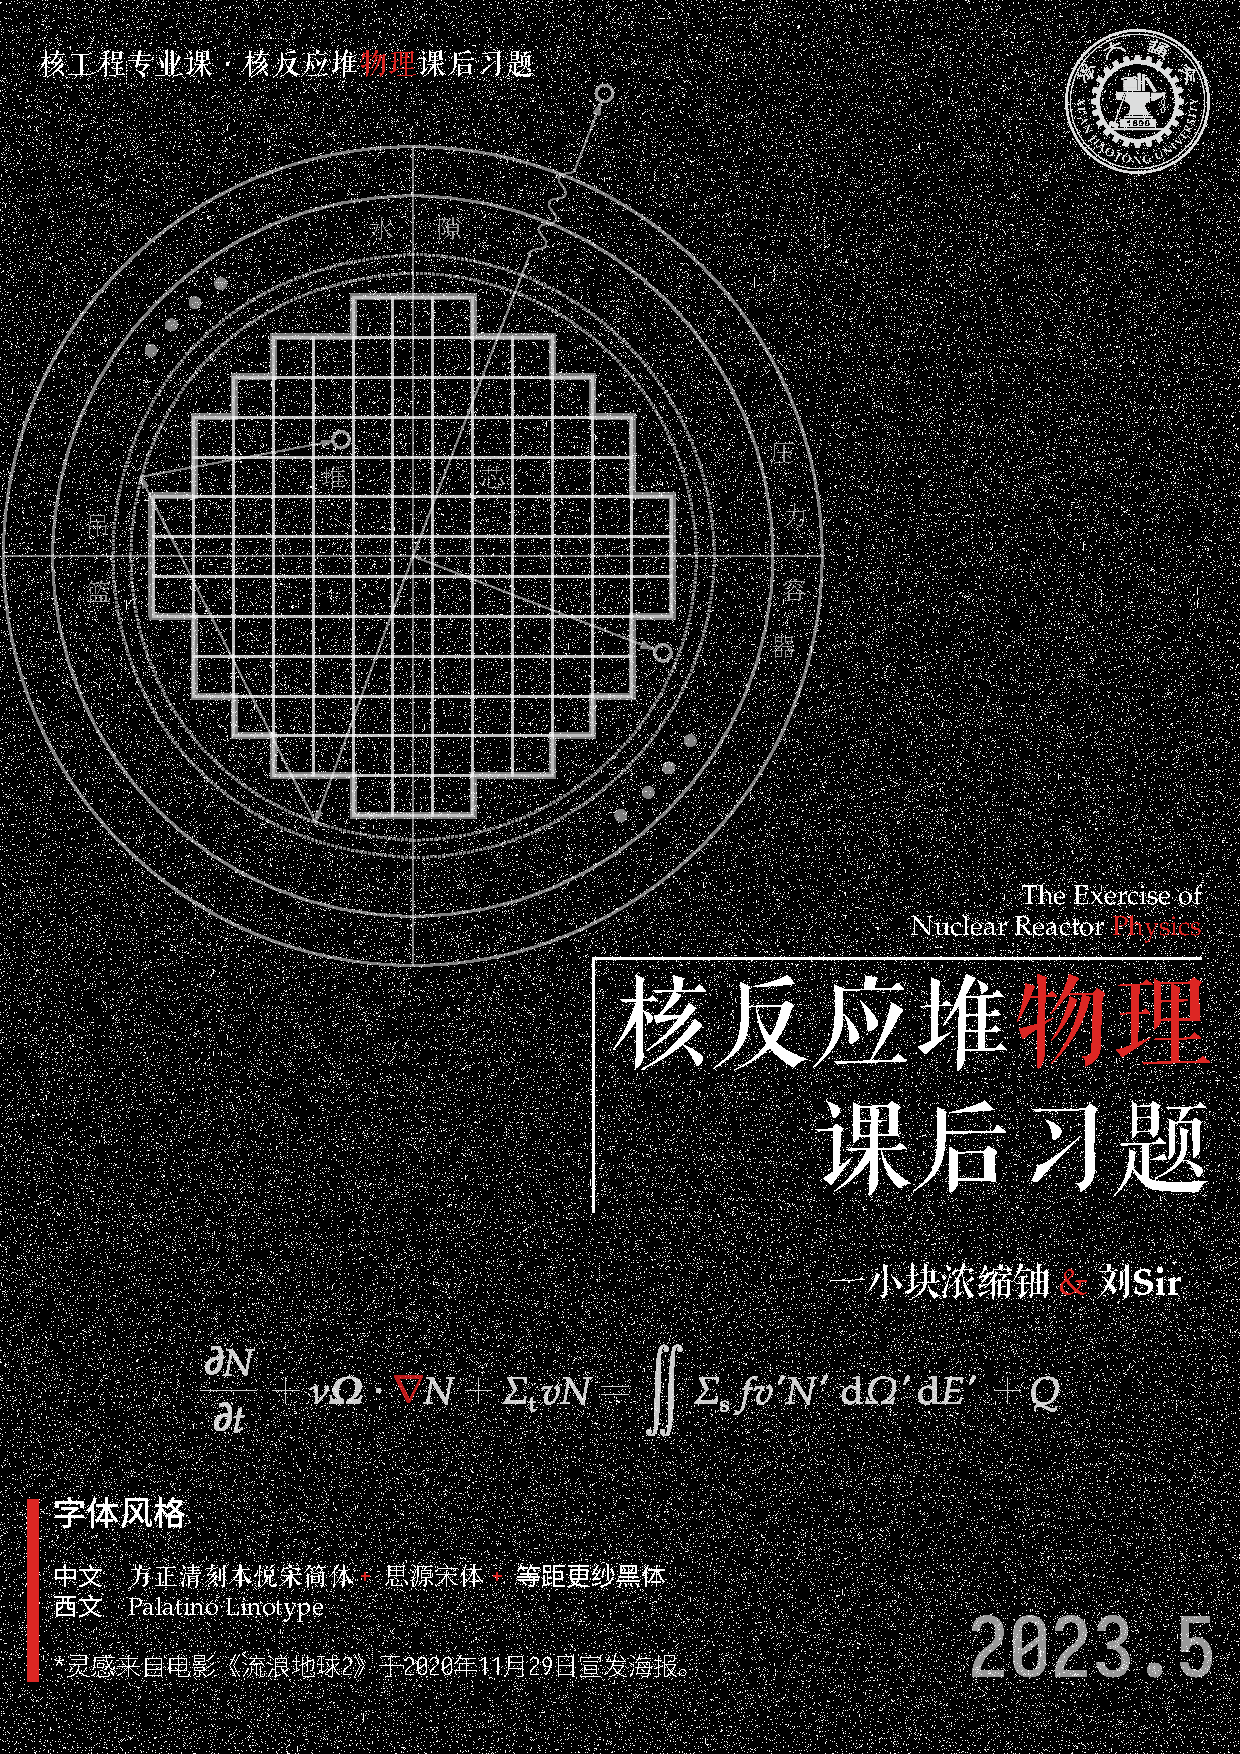
\includegraphics[width=\linewidth]{cover.jpg}
    % \vfill
    % \begin{center}
    %     \parbox{0.618\textwidth}{
    %     \hfill {\bfseries \Huge \thetitle} \\[0.6pt]  
    %     \rule{0.618\textwidth}{2pt} \\ 
    % }
    % \end{center}
    % \vfill
    % \begin{center}
    %     \parbox{0.618\textwidth}{
    %     \hfill\Large
    %     \kaishu 
    %       \begin{tabular}{r|}
    %       作者:\theauthor \\ 
    %       时间:\thedate \\
    %     \end{tabular}
    %     }
    % \end{center}
    % \vfill
    % \begin{center}
    %     \parbox[t]{0.7\textwidth}{\centering \kaishu }
    % \end{center}
    % \vfill
    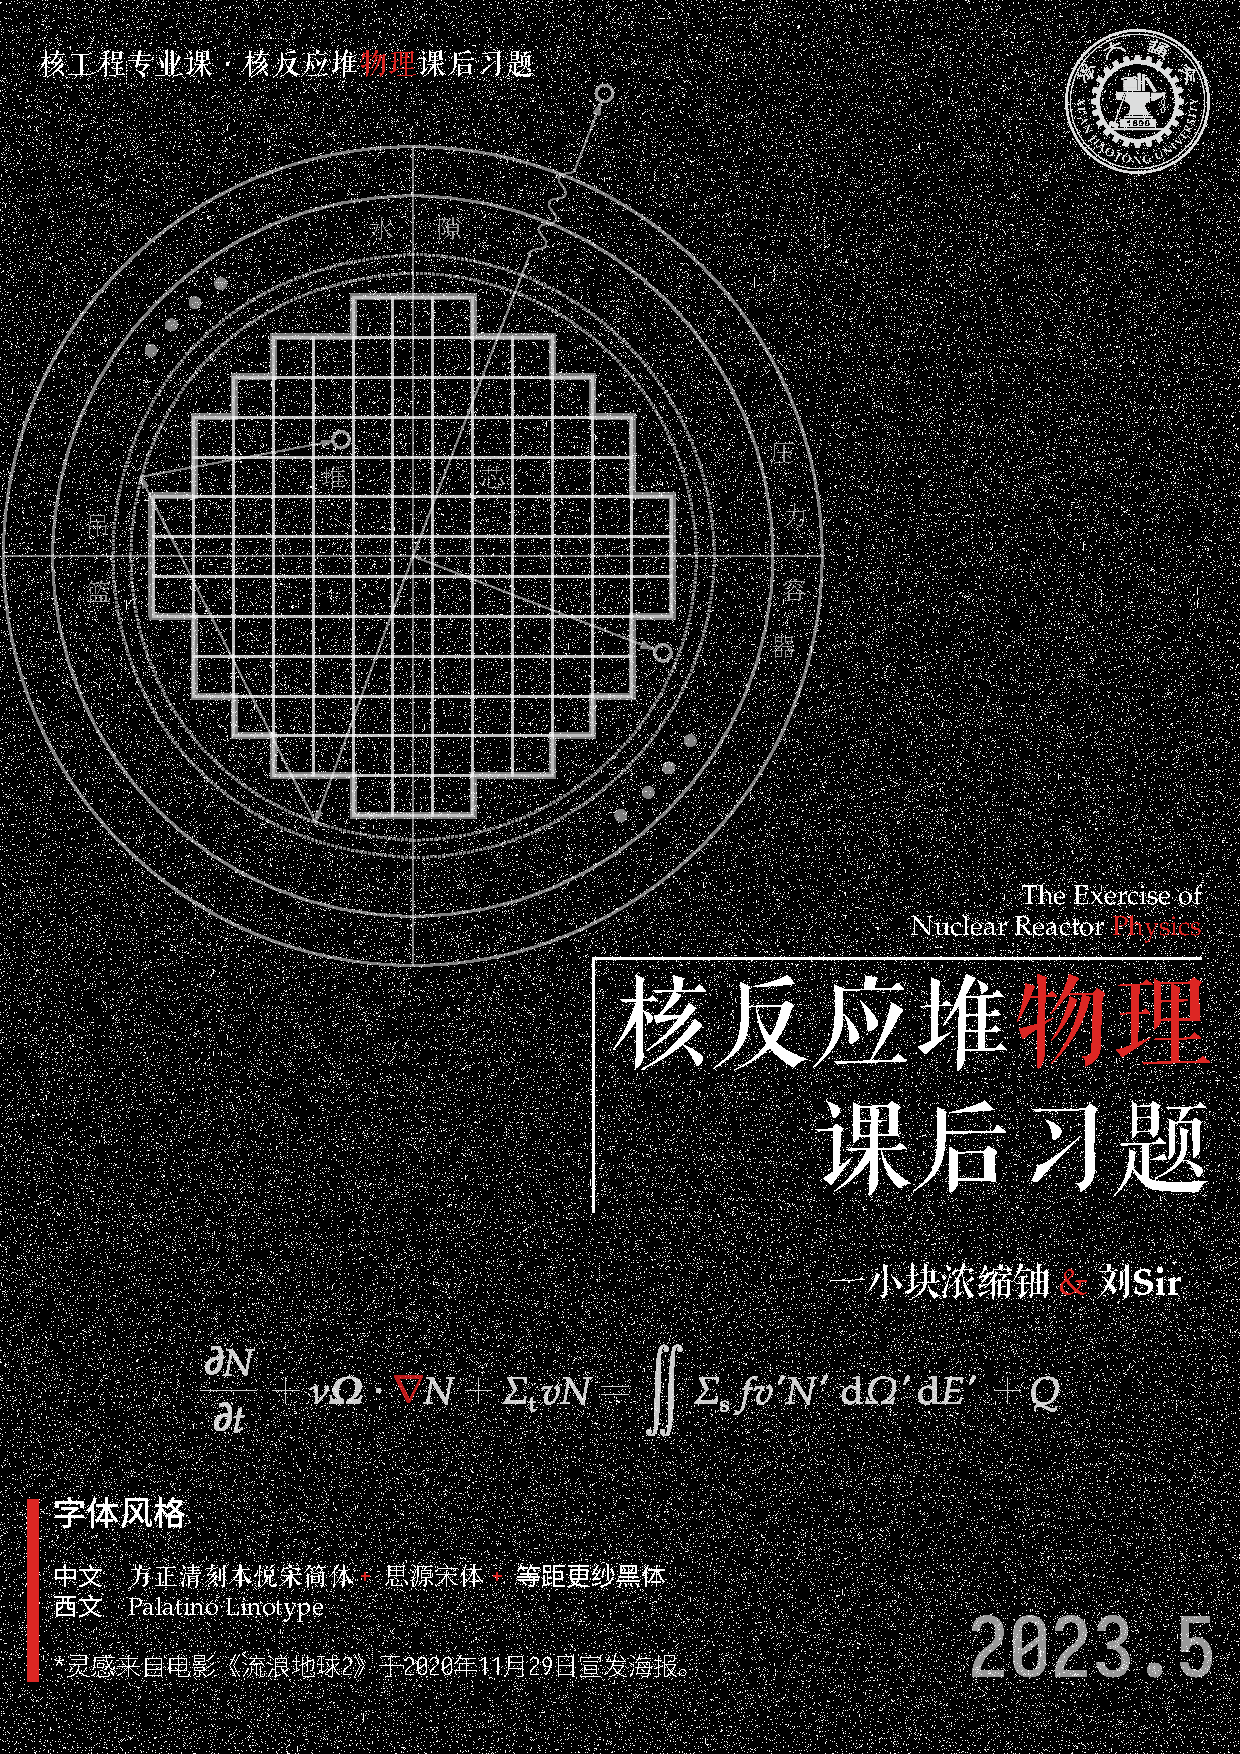
\includepdf{cover.pdf}
\end{titlepage}
}

\newcommand*{\keff}{k_{\symrm{eff}}}
\newcommand*{\dv}[2]{\frac{\symrm{d}{#1}}{\symrm{d}{#2}}}
\newcommand*{\ddv}[2]{\frac{\symrm{d^2}{#1}}{\symrm{d}{#2}^2}}
\newcommand*{\dd}[1]{\,\symrm{d}{#1}}
\newcommand*{\loge}{\symrm{ln}}
\newcommand*{\nsin}{\symrm{sin}}
\newcommand*{\ncos}{\symrm{cos}}
\newcommand*{\ntan}{\symrm{tan}}
\newcommand*{\vPhi}{\symit{\Phi}}
\newcommand*{\vSigma}{\symit{\Sigma}}
\newcommand*{\vLambda}{\symit{\Lambda}}
\newcommand*{\pddv}[2]{\frac{\symrm{\partial^2}{#1}}{\symrm{\partial}{#2}^2}}

\begin{document}

\title{核反应堆物理课后习题}
\author{一小块浓缩铀 \faRadiation*}
\date{\zhtoday}

\maketitle

\clearpage
\phantom{s}
\thispagestyle{empty}

\chapter*{写在前面}

《核反应堆物理》是西安交通大学核工程专业学生在大三下学期的必修课,旨在通过模拟核反应堆内中子与原子核的相互作用过程,为堆芯核设计、堆芯燃料管理、核反应堆运行、核反应堆启动试验、核反应堆安全分析等提供中子学基础数据。

这门课的期末考试题目主要来自于课本例题以及课后习题,课本例题已经由原书给出解答,我们希望通过这份资料给出课后习题的解答,帮助学习这门课的同学更好地完成作业以及高效的期末复习备考。

这份解答主要由\;{\kaishu 一小块浓缩铀}\;撰稿及排版,由\;{\kaishu 刘Sir}\;审核。因为我们水平有限,错漏之处在所难免,如果您发现有计算错误、笔误或其他需要改进之处,可以前往GitHub项目地址提供Issue或直接联系微信:

\begin{itemize}
    \item {\faGithub}:\,\href{https://github.com/Enriched-Uranium/Nuclear-Reactor-Physics}{https://github.com/Enriched-Uranium/Nuclear-Reactor-Physics}
    \item {\faWeixin}:\,XJTU-NEer
\end{itemize}

整份文档格式由\LaTeX{}排版,模板来自\href{https://zhuanlan.zhihu.com/p/601085820}{\faZhihu}作者Jiann,并在其基础上做了些许修改,图片使用Adobe illustrator和AxGlyph绘制。

酒红色文本均已嵌入超链接,点击即可跳转。

\begin{flushright}
    {\kaishu 一小块浓缩铀 \& 刘Sir} \\
    \zhtoday
\end{flushright}

\setcounter{tocdepth}{1}
\tableofcontents

\setcounter{page}{0}
\thispagestyle{empty}

\chapter{绪论}

\section*{习题}

\begin{exercise}
    什么是核反应堆?\,按照核反应堆发生的机理可分为哪几类?\,按照堆内的中子能谱可分为哪几类?\,按照冷却剂和慢化剂的种类可分为哪几类?\,
    \begin{solution}
        \begin{enumerate}[(1)]
            \item 核反应堆是指能以可控方式实现自持的链式裂变反应或核聚变反应的装置.
            \item 按照核反应堆发生的机理,核反应堆可分为裂变核反应堆、聚变核反应堆和聚变-裂变混合堆.
            \item 按照堆内的中子能谱,核反应堆可分为热中子堆和快中子堆.
            \item 按照冷却剂和慢化剂的种类,核反应堆可分为轻水堆(压水堆和沸水堆)、重水堆、气冷堆、液态金属堆等.
        \end{enumerate}
    \end{solution}
\end{exercise}

\begin{exercise}
    核反应堆物理分析的主要目标是什么?\,
    \begin{solution}
        核反应堆物理分析的主要目标是通过模拟核反应堆内中子与原子核的相互作用过程,为堆芯核设计、堆芯燃料管理、核反应堆运行、核反应堆启动试验、核反应堆安全分析等提供中子学基础数据.
    \end{solution}
\end{exercise}

\chapter{核反应堆核物理基础}

\section*{习题}

\begin{exercise}
    名词解释:\,易裂变核素,\,可转换核素,\,核反应率,\,中子注量率. 
    \begin{solution}
        \begin{enumerate}[(1)]
            \item 易裂变核素:\,可用任意小能量的中子引发裂变的核素,\,如${}^{233}\symrm{U},\,{}^{235}\symrm{U},\,{}^{239}\symrm{Pu}$等. 
            \item 可转换核素:\,俘获中子后经历一系列衰变成为易裂变核素的可裂变核素. 
            \item 核反应率:\,单位时间单位体积内所有中子与介质原子核发生反应的次数,\,即
            \begin{equation*}
                R = \vSigma \phi = \vSigma n v \quad (\symrm{m^{-3}\cdot s^{-1}})
            \end{equation*}
            \item 中子注量率:\,中子密度和中子速率的乘积,\,即
            \begin{equation*}
                \phi = n v \quad (\symrm{m^{-2}\cdot s^{-1}})
            \end{equation*}
        \end{enumerate}
    \end{solution}
\end{exercise}

\begin{exercise}
    在${}^{235}\symrm{U}$的裂变反应所发射的中子中,\,缓发中子的份额为($1\,\beta = 0.0065$).
\end{exercise}

\begin{exercise}
    密度为$1000\,\symrm{kg/m^3}$的水对于能量为$0.0253\,\symrm{eV}$的中子的宏观吸收截面约为多少?\,(已知H,\,O的热中子微观吸收截面分别为0.332\,b和0.00027\,b,\,阿伏伽德罗常数为$6.022 \times 10^{23}$)
    \begin{solution}
        水的相对分子质量为
        \begin{equation*}
            M_{\symrm{H_2O}} = 2 \times 1.00797 + 1 \times 15.9994 = 18.0153
        \end{equation*}
        单位体积内氧原子个数
        \begin{equation*}
            N_{\symrm{O}} = N_{\symrm{H_2O}} = \frac{\rho N_{\symrm{A}}}{M_{\symrm{H_2O}}} = \frac{10^6 \times 6.022 \times 10^{23}}{18.0153} = 3.343 \times 10^{28} \, \symrm{m^{-3}}
        \end{equation*}
        单位体积内氢原子个数
        \begin{equation*}
            N_{\symrm{H}} = 2 N_{\symrm{O}} = 2 \times 3.343 \times 10^{28} = 6.686 \times 10^{28} \, \symrm{m^{-3}}
        \end{equation*}
        于是
        \begin{equation*}
            \vSigma_{\symrm{a,\,H_2O}} = N_{\symrm{H}}\sigma_{a,\,H} + N_{\symrm{O}}\sigma_{a,\,O} = 6.686 \times 0.332 + 3.343 \times 0.00027 \, \symrm{m^{-1}} = 2.221\,\symrm{m^{-1}}
        \end{equation*}
    \end{solution}
\end{exercise}

\begin{exercise}
    某压水堆采用$\symrm{UO_2}$作燃料,\,其质量富集度为2.43\%,\,密度为$1.0\times 10^4\,\symrm{kg/m^3}$,\,试计算:\,当中子能量为0.0253\,eV时,\,$\symrm{UO_2}$的宏观吸收截面和宏观裂变截面(假设铀只有${}^{235}\symrm{U}$和${}^{238}\symrm{U}$,\,氧均为${}^{16}\symrm{O}$).\,
    \begin{solution}
        设${}^{235}\symrm{U}$原子核所占比例为$c_5$,\,则
        \begin{equation*}
            c_5 = \left[1+0.9874\left(\frac{1}{\varepsilon}-1\right)\right]^{-1} = \left[1+0.9874\left(\frac{1}{0.0243}-1\right)\right]^{-1} = 0.024602
        \end{equation*}
        $\symrm{UO_2}$相对分子质量
        \begin{equation*}
            M_{\symrm{UO_2}} = 235c_5 + 238(1-c_5) + 16\times 2 = 269.93
        \end{equation*}
        $\symrm{UO_2}$单位体积分子数
        \begin{equation*}
            N_{\symrm{UO_2}} = \frac{\rho N_{\symrm{A}}}{M_{\symrm{UO_2}}} = \frac{10^4 \times 6.022 \times 10^{23}}{269.93} \, \symrm{m^{-3}} = 2.231 \times 10^{28}\,\symrm{m^{-3}}
        \end{equation*}
        则
        \begin{align*}
            &N_5 = c_5 N_{\symrm{UO_2}} = 0.05489 \times 10^{28}\,\symrm{m^{-3}} \\
            &N_8 = (1-c_5) N_{\symrm{UO_2}} = 2.176 \times 10^{28}\,\symrm{m^{-3}} \\
            &N_{\symrm{O}} = 2 N_{\symrm{UO_2}} = 4.462 \times 10^{28}\,\symrm{m^{-3}}
        \end{align*}
        对于能量为0.0253\,eV的中子,\,查附录3得,\,$\sigma_{\symrm{a,\,U_5}} = 680.9\,\symrm{b},\,\sigma_{\symrm{f,\,U_5}} = 584.8925\,\symrm{b},\,\sigma_{\symrm{a,\,U_8}} = 2.7\,\symrm{b},\,\sigma_{\symrm{a,\,O}} = 2.7 \times 10^{-4}\,\symrm{b}$,\,故
        \begin{align*}
            &\vSigma_{\symrm{a,\,UO_2}} = N_5\sigma_{\symrm{a,\,U_5}} + N_8\sigma_{\symrm{a,\,U_8}} + N_{\symrm{O}}\sigma_{\symrm{a,\,O}} = 43.25\,\symrm{m^{-1}} \\
            &\vSigma_{\symrm{f,\,UO_2}} = N_5\sigma_{\symrm{f,\,U_5}} = 32.10\,\symrm{m^{-1}}
        \end{align*}
    \end{solution}
\end{exercise}

\begin{exercise}
    为得到1\,kWh的能量,\,需要多少质量的${}^{235}\symrm{U}$发生裂变?
    \begin{solution}
        设需要$m\,\symrm{kg}$的${}^{235}\symrm{U}$发生裂变,\,则
        \begin{equation*}
            \frac{m\times 10^3}{235} \times 6.022 \times 10^{23} \times 200 \times 10^6 \times 1.6 \times 10^{-19} = 10^3 \times 3600 \quad (\symrm{J})
        \end{equation*}
        解得
        \begin{equation*}
            m = 4.390 \times 10^{-8}\,\symrm{kg}
        \end{equation*}
    \end{solution}
\end{exercise}

\begin{exercise}
    有一座小型核电厂,\,电功率为150\,MW,\,设电厂的效率(电功率与热功率的比值)为30\%.\,假设发生裂变的核素为纯${}^{235}\symrm{U}$,\,且每次裂变释放出的能量为200\,MeV,\,试估算该电厂核反应堆额定功率运行1\,h所消耗的${}^{235}\symrm{U}$量.\,
    \begin{solution}
        设该电厂核反应堆额定功率运行1\,h消耗${}^{235}\symrm{U}$的质量为$m\,\symrm{kg}$,\,取俘获-裂变比$\alpha = 0.17$,\,则
        \begin{equation*}
            \frac{1}{1+\alpha} \cdot \frac{m\times 10^3}{235} \times 6.022 \times 10^{23} \times 200 \times 10^6 \times 1.6 \times 10^{-19} \times 30\% = 150 \times 10^6 \times 3600 \quad (\symrm{J})
        \end{equation*}
        解得
        \begin{equation*}
            m = 0.02568\,\symrm{kg}
        \end{equation*}
    \end{solution}
\end{exercise}

\begin{exercise}
    一座电厂的额定电功率$P_{\symrm{e}}$为1000\,MW,\,效率$\eta_{\symrm{e}}$(电功率与热功率的比值)为32\%,\,年负荷因子$\eta$(实际年发电量与额定年发电量的比值)为0.85.\,
    \begin{enumerate}[(1)]
        \item 若该电厂为核电厂,\,假设发生裂变的核素为纯${}^{235}\symrm{U}$,\,且每次裂变释放出的能量为200\,MeV,\,试估算该电厂一年需要消耗多少吨${}^{235}\symrm{U}$?
        \item 若该电厂为火电厂,\,已知标准煤的发热值为$Q=29.271\,\symrm{MJ/kg}$,\,试估算该电厂一年需要消耗多少吨标准煤?
    \end{enumerate}
    \begin{solution}
        \begin{enumerate}[(1)]
            \item 设该电厂一年需要消耗$m$吨${}^{235}\symrm{U}$,\,取俘获-裂变比$\alpha = 0.17$,\,则
            \begin{equation*}
                \frac{1}{1+\alpha} \cdot \frac{m\times 10^6}{235} \times 6.022 \times 10^{23} \times 200 \times 10^6 \times 1.6 \times 10^{-19} \times 32\% = 0.85 \times 1000 \times 10^6 \times 365 \times 24 \times 3600 \quad (\symrm{J})
            \end{equation*}
            解得
            \begin{equation*}
                m = 1.195\,\symrm{t}
            \end{equation*}
            \item 设该电厂一年需要消耗$M$吨标准煤,\,显然有$\eta_{\symrm{e}} M Q = \eta P_{\symrm{e}} t$,\,即
            \begin{equation*}
                32\% M \times 10^3 \times 29.271 \times 10^6 = 0.85 \times 1000 \times 10^6 \times 365 \times 24 \times 3600 \quad (\symrm{J})
            \end{equation*}
            解得
            \begin{equation*}
                M = 2.8618 \times 10^6\,\symrm{t}
            \end{equation*}
        \end{enumerate}
    \end{solution}
\end{exercise}

\begin{exercise}
    在纯水慢化剂中加了一些硼酸$\symrm{H_3BO_3}$,\,使其热中子吸收截面增加了10\%,\,若已知水的宏观热中子吸收截面为$\vSigma_{\text{水}} = 0.0221\,\symrm{cm^{-1}}$,\,硼酸的微观热中子吸收截面为$\sigma_{\text{硼酸}}=756\,\symrm{b}$和天然硼的相对原子质量$A_{\symrm{B}}=10.82$,\,试求此时慢化剂中的硼浓度$C_{\symrm{B}}$为多少ppm(1\,ppm的硼浓度是指1\,kg水中含1\,mg的天然硼)\,?
    \begin{solution}
        设硼酸浓度为$C_{\symrm{H_3BO_3}}\,\symrm{ppm}$,\,近似认为慢化剂密度仍然为水的密度$\rho = 10^3\,\symrm{kg/m^3}$,\,则
        \begin{equation*}
            N_{\symrm{H_3BO_3}} = \frac{\rho C_{\symrm{H_3BO_3}} \times 10^{-3} \times N_{\symrm{A}}}{M_{\symrm{H_3BO_3}}}
        \end{equation*}
        而
        \begin{equation*}
            M_{\symrm{H_3BO_3}} = 3 \times 1.00797 + 10.82 + 3 \times 15.9994 = 61.84211\,\symrm{g/mol}
        \end{equation*}
        由题意,\,$N_{\symrm{H_3BO_3}} \sigma_{\symrm{H_3BO_3}} = 0.1 \vSigma_{\text{水}}$,\,于是
        \begin{equation*}
            N_{\symrm{H_3BO_3}} = \frac{0.1 \times 0.0221 \times 100}{756 \times 10^{-28}}\,\symrm{m^{-3}} = 2.9233 \times 10^{24}\,\symrm{m^{-3}}
        \end{equation*}
        联立上述式,\,得
        \begin{equation*}
            C_{\symrm{H_3BO_3}} = 144.87\,\symrm{ppm}
        \end{equation*}
        在1\,kg水中,\,物质的量$n(\symrm{H_3BO_3}) = n(\symrm{B})$,\,故有
        \begin{equation*}
            \frac{C_{\symrm{B}}}{M_{\symrm{B}}} = \frac{C_{\symrm{H_3BO_3}}}{M_{\symrm{H_3BO_3}}}
        \end{equation*}
        解得
        \begin{equation*}
            C_{\symrm{B}} = 52.524\,\symrm{ppm}
        \end{equation*}
    \end{solution}
\end{exercise}

\begin{exercise}
    为什么裂变碎片一般都带有放射性?
    \begin{solution}
        裂变碎片大都是一些不稳定的丰中子核素,\,通常需要经历$\beta$衰变才能稳定.\,
    \end{solution}
\end{exercise}

\begin{exercise}
    一个典型的商用压水堆新堆中,\,若在一个短的时间间隔内发射出$10^5$个缓发中子,\,则在这同一时间内发射出的瞬发中子数大约为多少?
    \begin{solution}
        在以${}^{235}\symrm{U}$作核燃料的热中子核反应堆中,\,缓发中子份额$\beta = 0.0065$,\,故瞬发中子数为
        \begin{equation*}
            n_0 = \frac{10^5}{\beta} \cdot (1-\beta) = \frac{10^5}{0.0065} \cdot (1-0.0065) = 1.528 \times 10^{7}
        \end{equation*}
    \end{solution}
\end{exercise}

\begin{exercise}
    设某吸收剂的微观吸收截面$\sigma_{\symrm{a}}(E)$服从$1/v$定律,\,假定近似中子能谱可用$1/E$谱描述,\,试求该吸收剂第$g$群$(E_{g-1},\,E_g)$的平均微观吸收截面$\sigma_{\symrm{a}\,g}$.\,
    \begin{solution}
        由题意,\,$\sigma_{\symrm{a}}(E) \propto 1/v \propto 1/\sqrt{E}$,\,$\phi(E) \propto (1/E)$,\,于是
        \begin{equation*}
            \sigma_{\symrm{a}\,g} = \frac{\int_{E_{g-1}}^{E_g} \sigma_{\symrm{a}}(E) \phi(E) \dd{E}}{\int_{E_{g-1}}^{E_g} \phi(E) \dd{E}} \propto \frac{\int_{E_{g-1}}^{E_g} E^{-3/2} \dd{E}}{\int_{E_{g-1}}^{E_g} E^{-1} \dd{E}} = \frac{2\left(1/\sqrt{E_{g-1}} - 1/\sqrt{E_g}\right)}{\loge \left(E_g / E_{g-1}\right)}
        \end{equation*}
        将$\sigma_{\symrm{a}}(E) \propto 1/\sqrt{E},\,\phi(E) \propto 1/E$的比例系数全部归一为$C_{\sigma}$,\,则
        \begin{equation*}
            \sigma_{\symrm{a}\,g} = \frac{2 C_{\sigma} \left(1/\sqrt{E_{g-1}} - 1/\sqrt{E_g}\right)}{\loge \left(E_g / E_{g-1}\right)}
        \end{equation*}
    \end{solution}
\end{exercise}

\chapter{核反应堆中子学过程}
\section*{习题}

\begin{exercise}
    名词解释:\,有效增殖系数,\,慢化过程,\,扩散过程,\,中子流密度,\,中子慢化长度,\,中子扩散长度,\,中子徙动长度,\,中子慢化时间,\,中子扩散时间,\,中子平均寿命.\,
    \begin{solution}
        \begin{enumerate}[(1)]
            \item 有效增殖系数:\,一个系统内新生一代的中子数与产生它们的直属上一代中子数之比,\,即
            \begin{equation*}
                \keff = \frac{\text{新生一代中子数}}{\text{直属上一代中子数}} = \frac{\text{系统内中子产生率}}{\text{系统内中子总消失(吸收+泄漏)率}}
            \end{equation*}
            \item 慢化过程:\,中子能量不断减少,\,直至变成热中子的过程.\,
            \item 扩散过程:\,热中子在介质中位置不断变化的过程.\,
            \item 中子流密度:\,单位时间内沿着某一方向穿过单位面积的中子数,\,用$\vec{J}$表示.\,
            \item 中子慢化长度:\,无限均匀介质中,\,快中子从点源出发至慢化成热中子所穿行的直线距离方均值的$\frac{1}{6}$. 
            \item 中子扩散长度:\,无限均匀介质中,\,热中子从产生至被吸收时所穿行的直线距离方均值的$\frac{1}{6}$. 
            \item 中子徙动长度:\,无限均匀介质中,\,快中子从产生到被吸收时所穿行的直线距离方均值的$\frac{1}{6}$. 
            \item 中子慢化时间:\,裂变中子从裂变能慢化到热中子分界能$E_{\symrm{th}}$所需的平均时间,\,用$t_{\symrm{s}}$表示.\,
            \item 中子扩散时间:\,热中子扩散至被吸收所需的平均时间,\,用$t_{\symrm{d}}$表示.\,
            \item 中子平均寿命:\,快中子自裂变慢化到热中子,\,再扩散到被吸收所需的平均总时间,\,用$l$表示,\,$l = t_{\symrm{s}} + t_{\symrm{d}}$.\,
        \end{enumerate}
    \end{solution}
\end{exercise}

\begin{exercise}
    某裂变堆,\,快中子增殖因数1.05,\,逃脱共振吸收概率0.9,\,慢化不泄漏概率0.952,\,扩散不泄漏概率0.94,\,有效裂变中子数1.335,\,热中子利用系数0.882,\,试计算其无限介质增殖因数和有效增殖因数.\,
    \begin{solution}
        由题意,\,$\varepsilon = 1.05,\,p=0.9,\,P_{\symrm{s}}=0.952,\,P_{\symrm{d}}=0.94,\,\eta=1.335,\,f=0.882$,\,则
        \begin{align*}
            &k_{\infty} = \varepsilon p f \eta = 1.05 \times 0.9 \times 0.882 \times 1.335 = 1.1127 \\
            &\keff = k_{\infty} P_{\symrm{s}} P_{\symrm{d}} = 1.1127 \times 0.952 \times 0.94 = 0.9957
        \end{align*}
    \end{solution}
\end{exercise}

\begin{exercise}
    某热中子核反应堆处于临界状态,\,每次裂变产生中子数$\nu = 2.43$,\,已知该堆的中子泄漏损失占总中子数的10\%,\,试求:\,
    \begin{enumerate}[(1)]
        \item 用于维持裂变反应的中子数占总中子数的百分比$R_{\symrm{f}}$;
        \item 除裂变以外,\,被吸收的中子数占总中子数的百分比$R_{\symrm{a}}$; 
    \end{enumerate}
    \begin{solution}
        \begin{enumerate}[(1)]
            \item 堆处于临界状态,$\nu$个中子中,必须有1个中子来维持链式裂变反应,于是
            \begin{equation*}
                R_{\symrm{f}} = \frac{1}{\nu} = \frac{1}{2.43} = 0.4115
            \end{equation*}
            \item 剔除泄漏的$0.1\nu$个中子以及维持裂变的1个中子,于是
            \begin{equation*}
                R_{\symrm{a}} = \frac{\nu - 0.1\nu - 1}{\nu} = 0.4885
            \end{equation*}
        \end{enumerate}
    \end{solution}
\end{exercise}

\begin{exercise}
    核反应堆刚好临界时,\,$\keff = 1,\,\Delta k/k = 0$.
\end{exercise}

\begin{exercise}
    反应性的单位有哪些?
    \begin{solution}
        \begin{enumerate}[(1)]
            \item $1\,\symrm{pcm} = 10^{-5}$;
            \item $1\,\symrm{mk} = 10^{-3}$;
            \item $1\,\$ = 1\,\beta = 0.0065$(不是固定值).
        \end{enumerate}
    \end{solution}
\end{exercise}

\begin{exercise}
    操作员从堆中将控制棒提出,\,使得核反应堆的有效增殖因子$\keff$从0.998变为1.002,\,此核反应堆处于\xparen
    \begin{xchoices}[showanswer=true]
        \item 瞬发临界
        \item* 超临界
        \item 刚好临界
        \item 次临界
    \end{xchoices}
    \vspace{1em}
    \noindent {\color{third}{【注】}} {\kaishu 瞬发临界是指$\rho = \beta$,\,进一步,\,瞬发超临界是指$\rho > \beta$.}
\end{exercise}

\begin{exercise}
    在一个运行着的核反应堆堆芯中,\,一个热中子即将与一个铀-238核相互作用.\,以下哪一种情形最有可能发生,\,并且将怎样影响堆芯的$\keff$?\xparen
    \begin{xchoices}[showanswer=true]
        \item 该中子将被散射,\,使$\keff$不变
        \item 该中子将被吸收,\,铀-238核将裂变,\,使$\keff$减小
        \item 该中子将被吸收,\,铀-238核将裂变,\,使$\keff$增大
        \item* 该中子将被吸收,\,铀-238核将衰变,\,生成钚-239,\,使$\keff$增大
    \end{xchoices}
    \vspace{1em}
    \noindent {\color{third}{【注】}} {\kaishu 此题有争议,尚未解决。个人认为按截面大小比较,应该选A,但似乎助教是按D批改的。}
\end{exercise}

\begin{exercise}
    为使铀的有效裂变中子数$\eta=1.7$,\,试采用$E_{\symrm{n}}=0.0253\,\symrm{eV}$时的截面估计铀中${}^{235}\symrm{U}$的质量富集度.\,
    \begin{solution}
        对于$E_{\symrm{n}}=0.0253\,\symrm{eV}$的热中子,\,只有${}^{235}\symrm{U}$发生裂变,\,则有效裂变中子数
        \begin{equation*}
            \eta = \frac{\nu \vSigma_{\symrm{f5}}}{\vSigma_{\symrm{a5}}+\vSigma_{\symrm{a8}}} = \frac{\nu N_5 \sigma_{\symrm{f5}}}{N_5 \sigma_{\symrm{a5}} + N_8 \sigma_{\symrm{a8}}}
        \end{equation*}
        可以得到
        \begin{equation*}
            \frac{N_8}{N_5} = \frac{\nu \sigma_{\symrm{f5}} - \eta \sigma_{\symrm{a5}}}{\eta \sigma_{\symrm{a8}}}
        \end{equation*}
        进一步
        \begin{equation*}
            c_5 = \frac{N_5}{N_5+N_8} = \frac{1}{1+\frac{N_8}{N_5}} = \frac{\eta \sigma_{\symrm{a8}}}{\nu \sigma_{\symrm{f5}} - \eta \sigma_{\symrm{a5}} + \eta \sigma_{\symrm{a8}}}
        \end{equation*}
        代入$\eta = 1.7$,\,查附录3,\,得$\sigma_{\symrm{a8}}=2.6828\,\symrm{b},\,\sigma_{\symrm{a5}}=683.5565\,\symrm{b},\,\sigma_{\symrm{f5}} = 584.8925\,\symrm{b}$,\,取$\nu = 2.43$,\,得$c_5 = 0.0172885$.
        故铀中${}^{235}\symrm{U}$的质量富集度
        \begin{equation*}
            \varepsilon = \frac{235c_5}{235c_5+238(1-c_5)} = 0.01707 = 1.707\%
        \end{equation*}
    \end{solution}
\end{exercise}

\begin{exercise}
    某核反应堆堆芯内的平均宏观裂变截面为$5\,\symrm{m^{-1}}$,\,平均功率密度为$20\,\symrm{MW/m^3}$;\,假设每次裂变释放出的能量为200\,MeV,\,试求堆芯内的平均中子注量率.\,
    \begin{solution}
        由题意,\,$\vSigma_{\symrm{f}} = 5\,\symrm{m^{-1}},\,P_V = 20\,\symrm{MW/m^3} = 2\times 10^7\,\symrm{J/(m^3 \cdot s)},\,E_0 = 200\,\symrm{MeV} = 3.2\times 10^{-11}\,\symrm{J}$.\,由$P_V = \vSigma_{\symrm{f}} \overline{\phi} E_0$,\,得
        \begin{equation*}
            \overline{\phi} = \frac{P_V}{\vSigma_{\symrm{f}} E_0} = \frac{2\times 10^7}{5\times 3.2\times 10^{-11}}\,\symrm{m^{-2}\cdot s^{-1}} = 1.25 \times 10^{17}\,\symrm{m^{-2}\cdot s^{-1}}
        \end{equation*}
    \end{solution}
\end{exercise}

\begin{exercise}
    H和O在1000\,eV到1\,eV能量范围内的散射截面近似为常数,\,分别为20\,b和38\,b.\,计算$\symrm{H_2O}$的平均对数能降增量以及中子在$\symrm{H_2O}$中从1000\,eV慢化到1\,eV所需的平均碰撞次数.\,
    \begin{solution}
        平均对数能降增量
        \begin{equation*}
            \xi = 1 - \frac{(A-1)^2}{2A}\loge\left(\frac{A+1}{A-1}\right)
        \end{equation*}
        于是有$\xi_{\symrm{H}}=1,\,\xi_{\symrm{O}}=0.1199$.
        轻水的慢化能力来自氢核,\,氧核两方面的贡献,\,即
        \begin{align*}
            &\xi_{\symrm{H_2O}}\vSigma_{s,\,H_2O} = \xi_{\symrm{H}}\vSigma_{s,\,H} + \xi_{\symrm{O}}\vSigma_{s,\,O} \\
            \Rightarrow & \xi_{\symrm{H_2O}}(N_{\symrm{H}}\sigma_{\symrm{s,H}} + N_{\symrm{O}}\sigma_{\symrm{s,O}}) = \xi_{\symrm{H}}N_{\symrm{H}}\sigma_{\symrm{s,H}} + \xi_{\symrm{O}}N_{\symrm{O}}\sigma_{\symrm{s,O}}
        \end{align*}
        $N_{\symrm{H}}=2N_{\symrm{O}}$,\,两边同除以$N_{\symrm{O}}$,\,得
        \begin{equation*}
            \xi_{\symrm{H_2O}}(2\sigma_{\symrm{s,H}} + \sigma_{\symrm{s,O}}) = 2\xi_{\symrm{H}}\sigma_{\symrm{s,H}} + \xi_{\symrm{O}}\sigma_{\symrm{s,O}}
        \end{equation*}
        即
        \begin{equation*}
            \xi_{\symrm{H_2O}} = \frac{2\xi_{\symrm{H}}\sigma_{\symrm{s,H}} + \xi_{\symrm{O}}\sigma_{\symrm{s,O}}}{2\sigma_{\symrm{s,H}} + \sigma_{\symrm{s,O}}} = \frac{2\times 1\times 20 + 0.1199\times 38}{2\times 20 + 38} = 0.5712
        \end{equation*}
        平均碰撞次数
        \begin{equation*}
            N_{\symrm{c,\,H_2O}} = \frac{\loge \frac{E_1}{E_2}}{\xi_{\symrm{H_2O}}} = \frac{\loge \frac{1000}{1}}{0.5712} = 12.09
        \end{equation*}
    \end{solution}
\end{exercise}

\chapter{中子扩散理论与计算}
\section*{习题}

\begin{exercise}
    试总结中子扩散理论的适用范围。
    \begin{solution}
        \begin{enumerate}[(1)]
            \item 介质无限均匀;
            \item 在L系内散射各向同性;
            \item 介质弱吸收;
            \item 中子注量率分布变化缓慢。
        \end{enumerate}
    \end{solution}
\end{exercise}

\begin{exercise}
    有两束方向相反的平行热中子束射到${}^{235}\symrm{U}$薄片上,设其上某点自左面入射的中子束强度为$10^{12}\,\symrm{cm^{-2}\cdot s^{-1}}$,自右面入射的中子束强度$2 \times 10^{12}\,\symrm{cm^{-2}\cdot s^{-1}}$。计算:
    \begin{enumerate}[(1)]
        \item 该点的中子注量率;
        \item 该点的中子流密度;
        \item 设$\vSigma_{\symrm{a}} = 19.2 \times 10^2\,\symrm{m^{-1}}$,求该点的吸收率。
    \end{enumerate}
    \begin{solution}
        \begin{figure}[H]
            \centering
            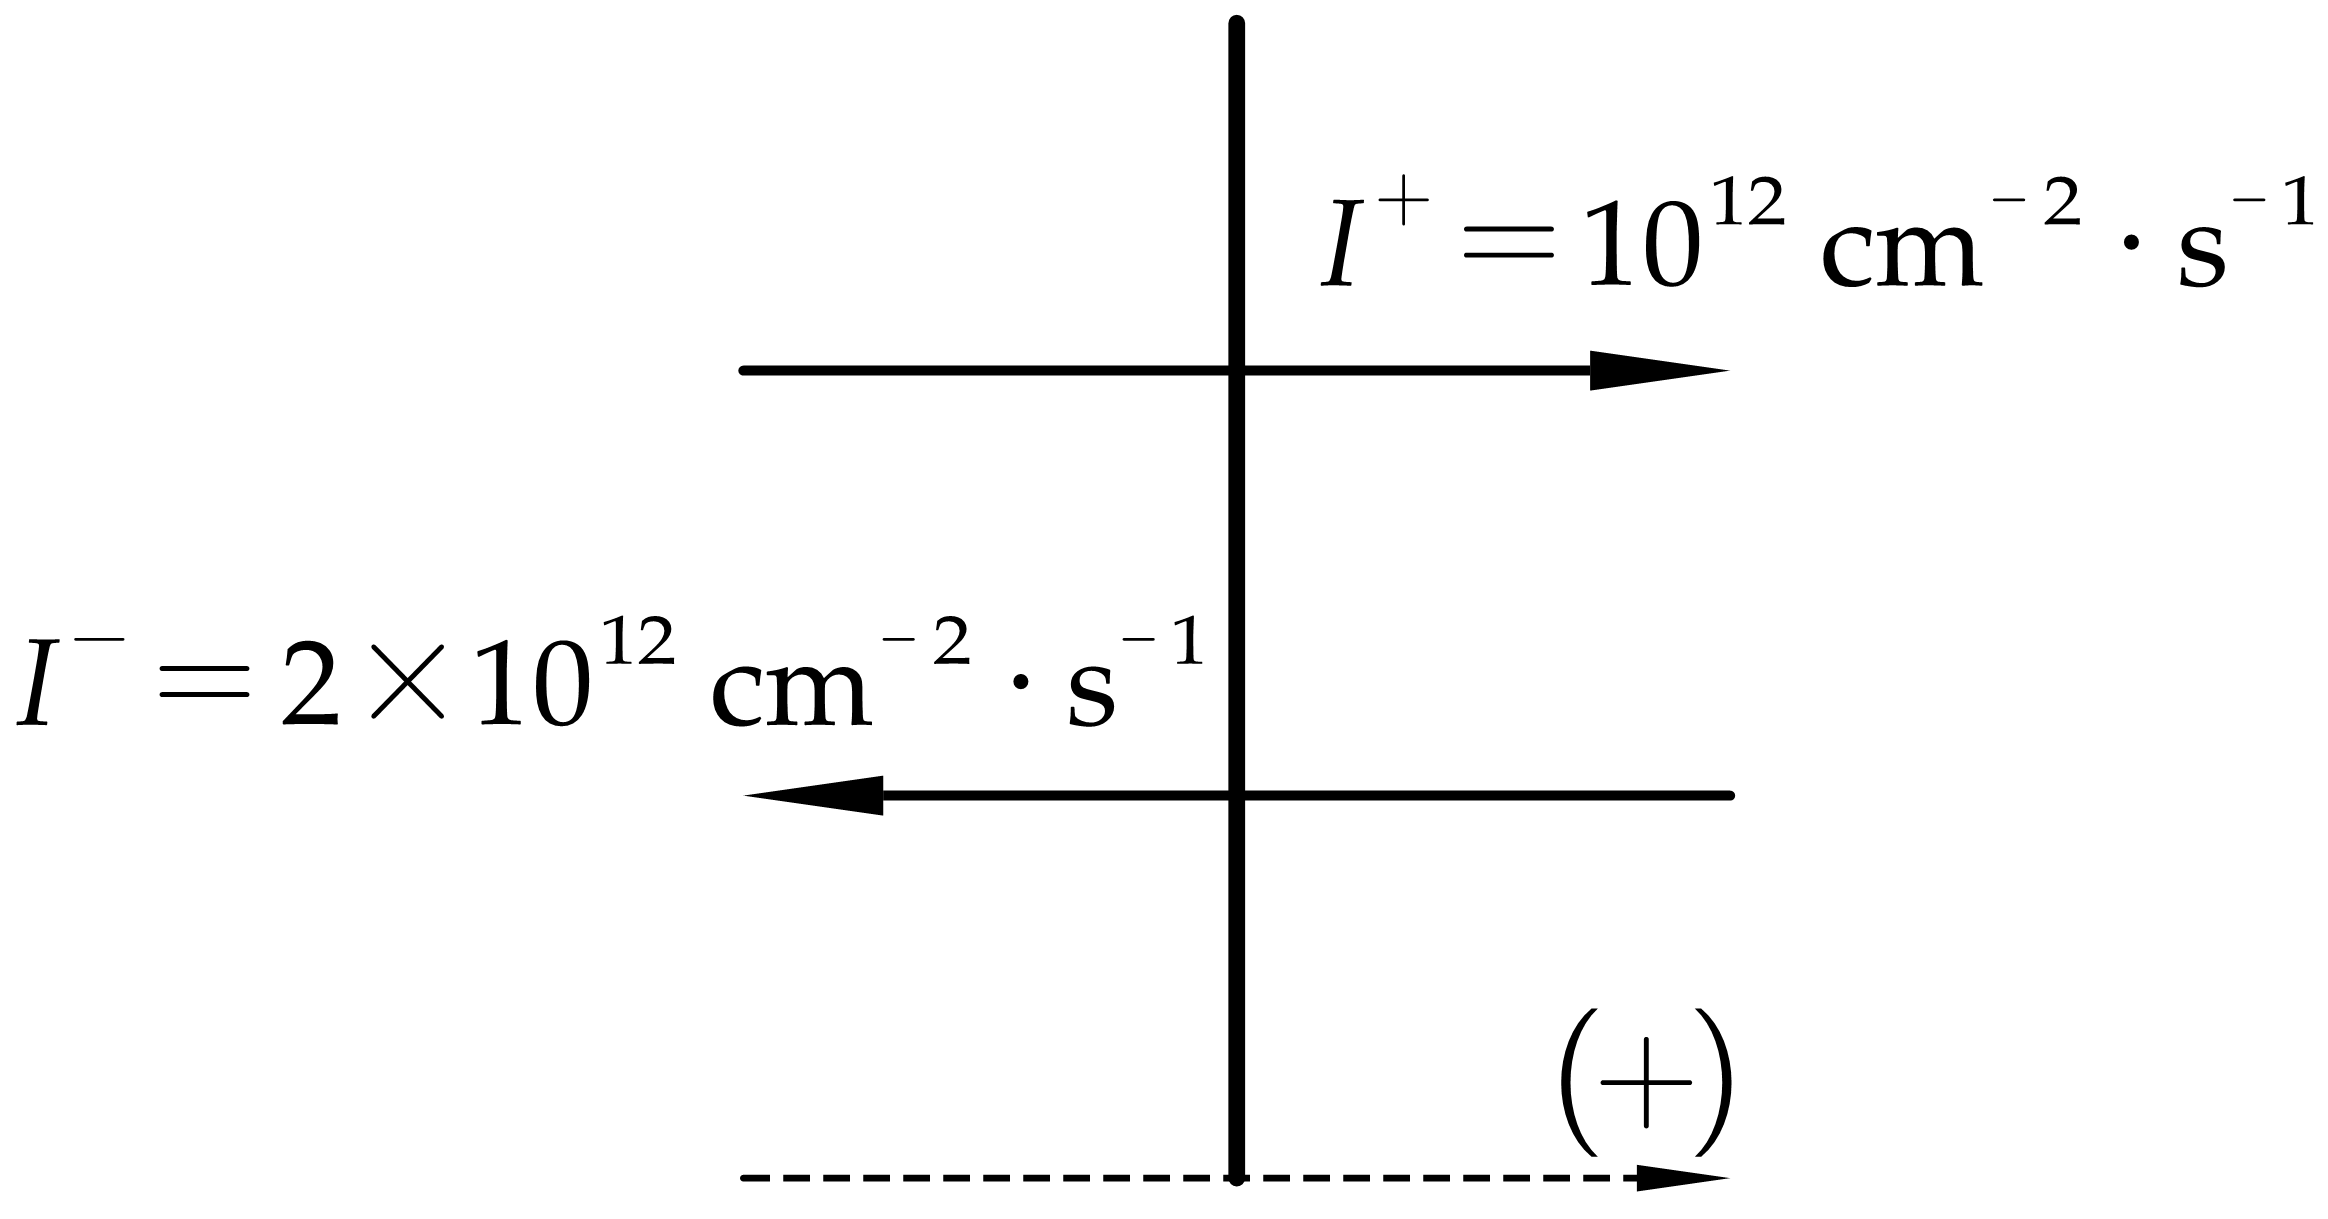
\includegraphics[scale=1.5]{figures/fig4.2.png}
        \end{figure}
        如图所示,取水平向右为正方向,则
        \begin{enumerate}[(1)]
            \item $\phi = I^{+} + I^{-} = 3\times 10^{12}\,\symrm{cm^{-2}\cdot s^{-1}}$;
            \item $J = I^{+} - I^{-} = -10^{12}\,\symrm{cm^{-2}\cdot s^{-1}}$,\,负号表示其方向与正方向相反;
            \item $R_{\symrm{a}} = \vSigma_{\symrm{a}}\phi = 19.2\times 3\times 10^{12}\,\symrm{cm^{-3}\cdot s^{-1}} = 5.76\times 10^{13}\,\symrm{cm^{-3}\cdot s^{-1}}$.
        \end{enumerate}
    \end{solution}
\end{exercise}

\begin{exercise}
    在某球形裸堆($R=0.5\,\symrm{m}$)内中子注量率分布为:
    \begin{equation*}
        \phi(r) = \frac{5\times 10^{13}\,\symrm{cm^{-1}\cdot s^{-1}}}{r} \nsin \left(\frac{\pi r}{R}\right)\,\symrm{cm^{-2}\cdot s^{-1}}
    \end{equation*}
    试求:
    \begin{enumerate}[(1)]
        \item $\phi(0)$;
        \item $J(r)$的表达式,设$D = 0.8\times 10^{-2}\,\symrm{m}$;
        \item 每秒从堆表面泄漏的总中子数(假设外推距离很小可忽略不计)。
    \end{enumerate}
    \begin{solution}
        \begin{enumerate}[(1)]
            \item \begin{equation*}
                \phi = \lim_{r\to 0} \frac{5\times 10^{13}}{r} \nsin \left(\frac{\pi r}{R}\right) = \lim_{r\to 0} \frac{5\times 10^{13}}{r} \cdot \frac{\pi r}{R} = 5\times 10^{13} \times \frac{\pi}{50}\,\symrm{cm^{-2}\cdot s^{-1}} = \pi \times 10^{12}\,\symrm{cm^{-2}\cdot s^{-1}}
            \end{equation*}
            \item $D = 0.8\times 10^{-2}\,\symrm{m} = 0.8\,\symrm{cm}$
            \begin{equation*}
                J(r) = -D\nabla \phi(r) = -D \dv{\phi(r)}{r} = 4\times 10^{13} \left[\frac{1}{r^2}\nsin \left(\frac{\pi r}{50}\right) - \frac{\pi}{50 r} \ncos\left(\frac{\pi r}{50}\right)\right]\,\symrm{cm^{-2}\cdot s^{-1}}
            \end{equation*}
            \item \begin{equation*}
                L = J(R)\cdot 4\pi R^2 = 4\times 10^{13} \left[\frac{1}{50^2}\nsin \left(\frac{50 \pi}{50}\right) - \frac{\pi}{50 \times 50} \ncos\left(\frac{50\pi}{50}\right)\right]\times 4\pi\times 50^2 \,\symrm{s^{-1}} = 1.579\times 10^{15}\,\symrm{s^{-1}}
            \end{equation*}
        \end{enumerate}
    \end{solution}
\end{exercise}

\begin{exercise}
    无限纯吸收介质(中子扩散系数为$D$,中子平均自由程为$\lambda$)内,在坐标$(-a,\,0,\,0)$和$(a,\,0,\,0)$处分别有两个源强为$S\,\symrm{s^{-1}}$的点源,试求坐标原点$P_1$和坐标$(0,\,a,\,0)\,P_2$处的中子注量率和中子流密度。
    \begin{solution}
        取$xy$平面,如图所示
        \begin{figure}[H]
            \centering
            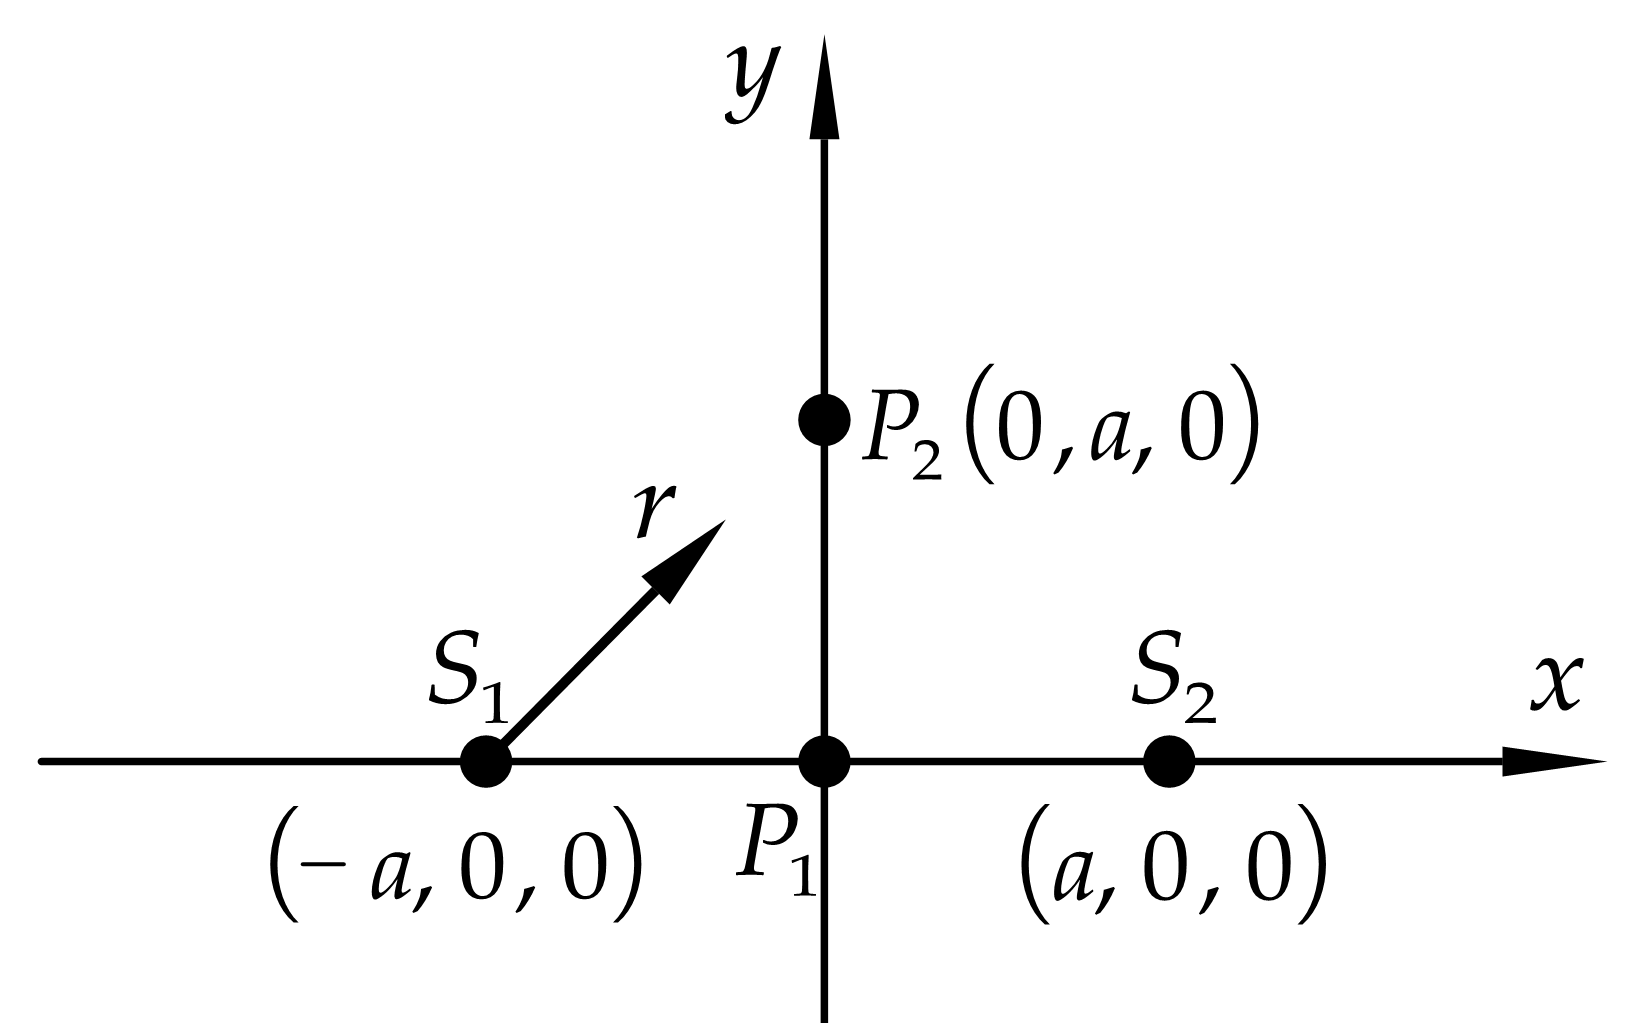
\includegraphics[scale=1.5]{figures/fig4.4.png}
        \end{figure}
        以$S_1$为原点建立一维球坐标系$S_1-r$,则单能中子稳态扩散方程
        \begin{equation*}
            \nabla^2\phi(r)-\frac{\phi(r)}{L^2} = 0,\,r>0
        \end{equation*}
        其中,$r^2 = (x+a)^2+y^2$,$x\neq -a$且$y\neq 0$。

        通解为
        \begin{equation*}
            \phi(r) = A\frac{\symrm{e}^{-r/L}}{r} + C\frac{\symrm{e}^{r/L}}{r}
        \end{equation*}
        边界条件
        \begin{enumerate}[(a)]
            \item $\phi(r)$为有限正值,于是$C=0$;
            \item $\lim\limits_{r\to 0} J(r)\cdot 4\pi r^2 = S$
        \end{enumerate}

        解得
        \begin{align*}
            &J(r) = \frac{S}{4\pi r}\left(\frac{1}{L}+\frac{1}{r}\right)\symrm{e}^{-r/L} = \frac{S}{4\pi r}\left(\frac{1}{L}+\frac{1}{r}\right)\symrm{e}^{-r/\sqrt{D\lambda}} \\
            &\phi(r) = \frac{S\symrm{e}^{-r/L}}{4\pi D r} = \frac{S\symrm{e}^{-r/\sqrt{D\lambda}}}{4\pi D r}
        \end{align*}
        $S_2$与$S_1$源强相等且对称,则
        \begin{enumerate}[(1)]
            \item $P_1$点
            \begin{align*}
                &J_{P_1} = 0 \\
                &\phi_{P_1} = 2\phi(a) = \frac{S\symrm{e}^{-a/\sqrt{D\lambda}}}{2\pi D a}
            \end{align*}
            \item $P_2$点
            \begin{align*}
                &J_{P_2} = \sqrt{2}J(\sqrt{2}a) = \frac{S}{4\pi a}\left(\frac{1}{L}+\frac{1}{\sqrt{2}a}\right)\symrm{e}^{-\sqrt{2}a/\sqrt{D\lambda}} \\
                &\phi_{P_2} = 2\phi(\sqrt{2}a) = \frac{\sqrt{2}S\symrm{e}^{-\sqrt{2}a/\sqrt{D\lambda}}}{4\pi D a}
            \end{align*}
        \end{enumerate}
    \end{solution}
\end{exercise}

\begin{exercise}
    试求边长为$a,\,b,\,c$(包括外推距离)的长方体裸堆的几何曲率和中子注量率分布。设有一边长$a = b = 0.5\,\symrm{m},\,c = 0.6\,\symrm{m}$(包括外推距离)的长方体裸堆,$L = 0.0434\,\symrm{m},\,\tau = 6\,\symrm{cm^2}$。
    \begin{enumerate}[(1)]
        \item 求达到临界时所必需的$k_{\infty}$;
        \item 如果功率为$5000\,\symrm{kW},\,\vSigma_{\symrm{f}} = 4.01\,\symrm{m^{-1}}$,假设每次裂片释放出的能量为$200\,\symrm{MeV}$,求中子注量率分布。
    \end{enumerate}
    \begin{solution}
        以长方体几何中心为坐标原点建立空间直角坐标系$Oxyz$,如图所示
        \begin{figure}[H]
            \centering
            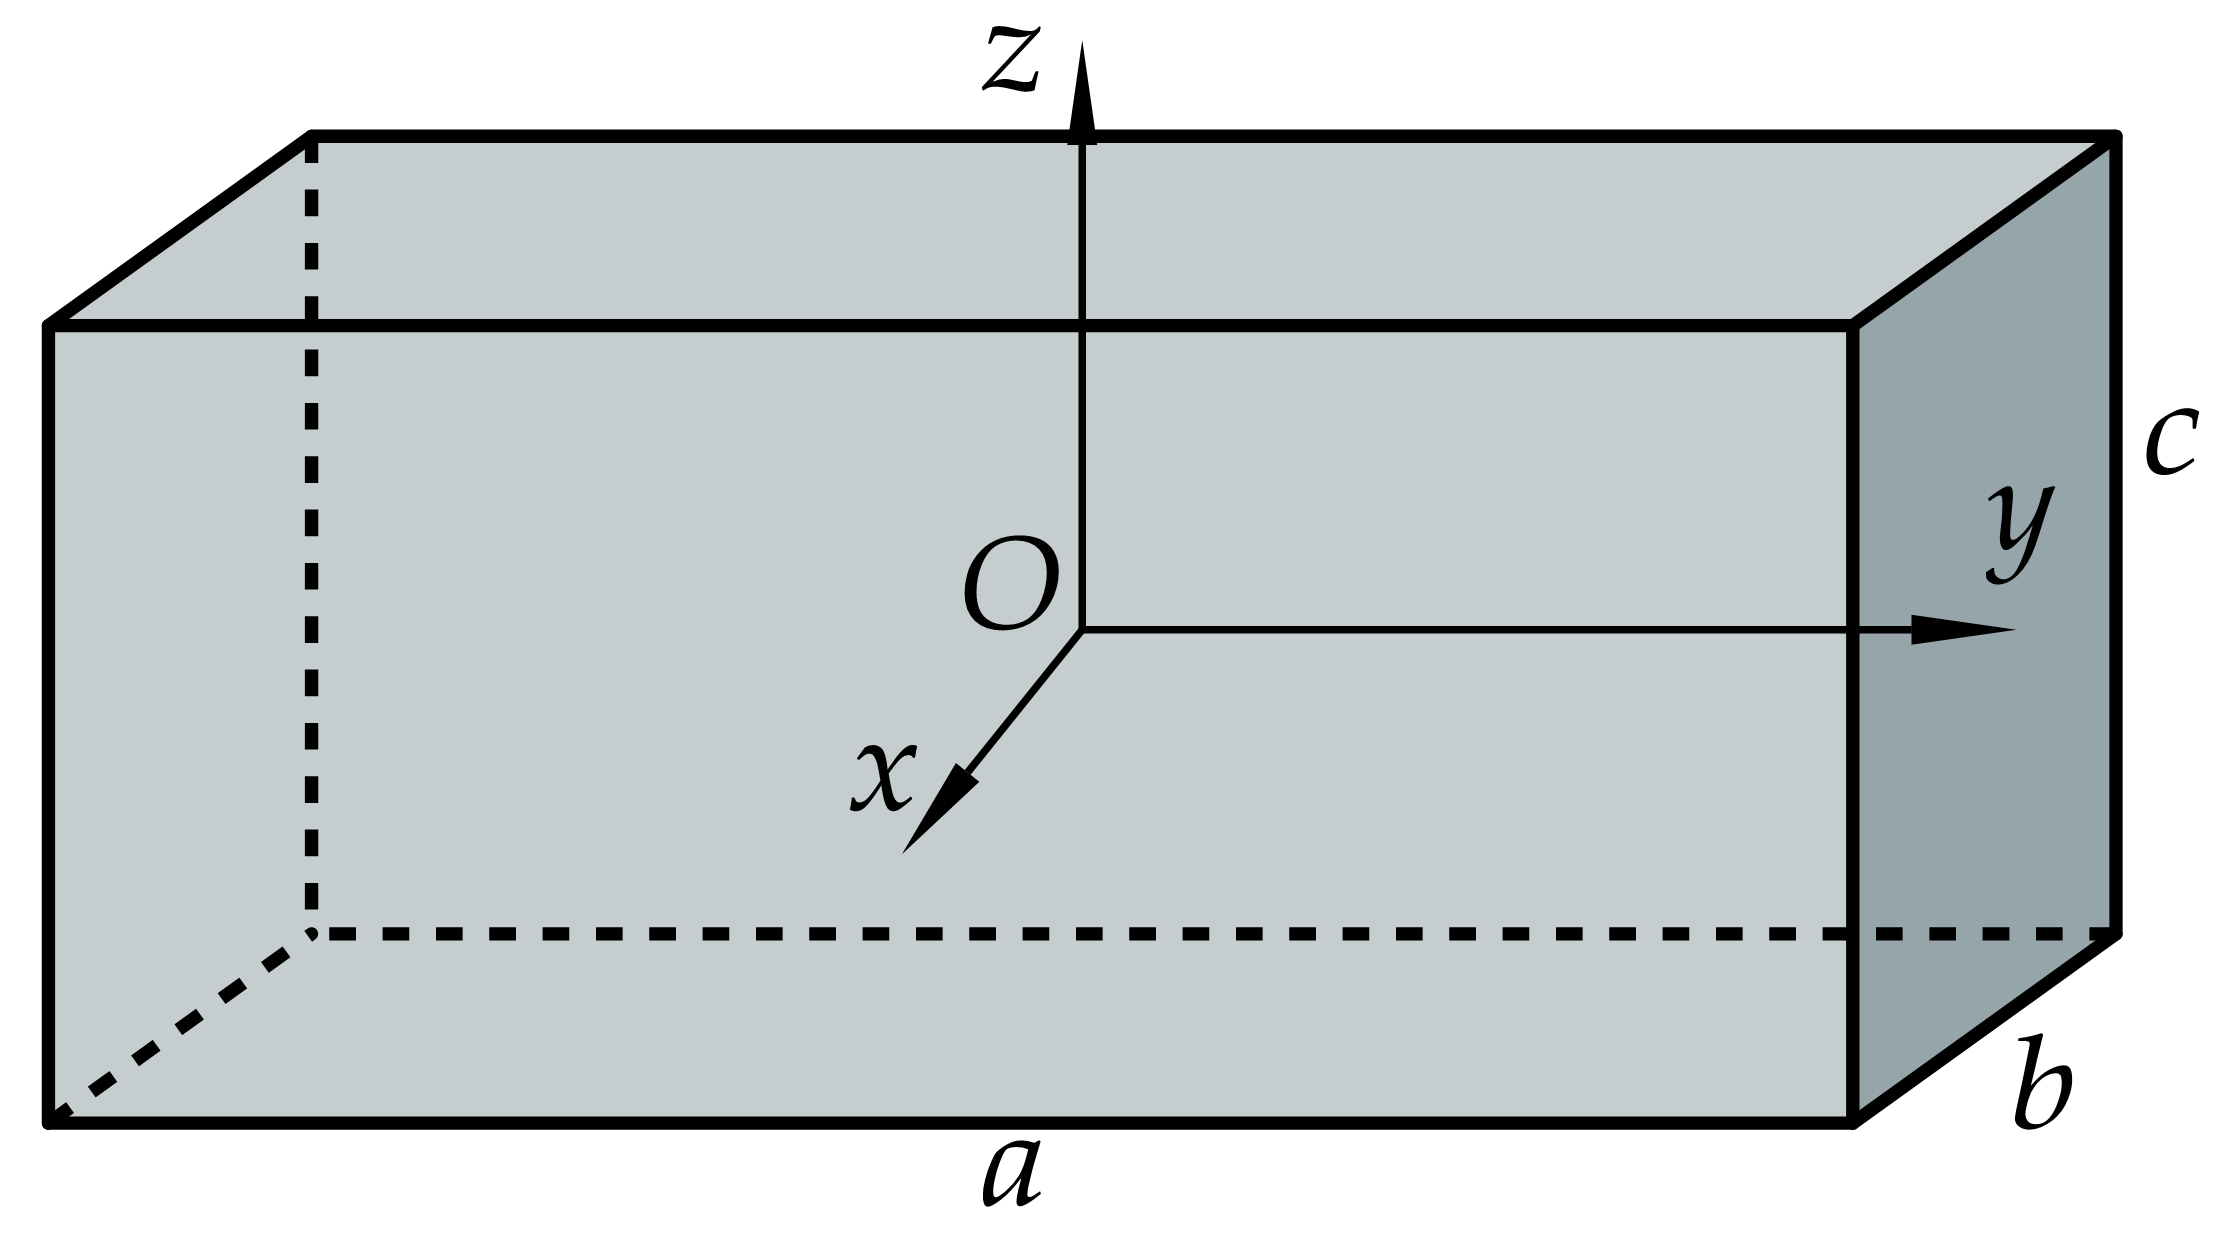
\includegraphics[scale=1]{figures/fig4.5.png}
        \end{figure}
        单能稳态中子扩散方程
        \begin{equation*}
            D\left(\pddv{\phi}{x}+\pddv{\phi}{y}+\pddv{\phi}{z}\right) - \vSigma_{\symrm{a}}\phi + k_{\infty}\vSigma_{\symrm{a}}\phi = 0
        \end{equation*}

        边界条件
        \begin{equation*}
            \phi\left(\pm \frac{a}{2},\,y,\,z\right) = \phi\left(x,\,\pm \frac{b}{2},\,z\right) = \phi\left(x,\,y,\,\pm \frac{c}{2}\right) = 0
        \end{equation*}

        分离变量$\phi(x,\,y,\,z) = \varphi_x(x)\varphi_y(y)\varphi_y(y)$,代入扩散方程,得
        \begin{equation*}
            \frac{\nabla^2\varphi_x(x)}{\varphi_x(x)} + \frac{\nabla^2\varphi_y(y)}{\varphi_y(y)} + \frac{\nabla^2\varphi_z(z)}{\varphi_z(z)} = -\frac{k_{\infty}-1}{L^2}
        \end{equation*}

        令
        \begin{equation*}
            \frac{\nabla^2\varphi_x(x)}{\varphi_x(x)} = -B_x^2 \Rightarrow \nabla^2\varphi_x(x) + B_x^2\varphi_x(x) = 0
        \end{equation*}
        通解为$\varphi_x(x) = A_{nx}\ncos B_{nx}x + C_{nx}\nsin B_{nx}x$。

        \begin{enumerate}[(a)]
            \item 由通量对称分布,得$C_{nx}=0$;
            \item 由边界条件,得$\varphi_x(a/2) = A_{nx}\ncos(aB_{nx}/2) = 0 \Rightarrow B_{nx} = \frac{(2n-1)\pi}{a}\,n=1,\,2,\,3,\,\cdots$.
        \end{enumerate}

        稳态时,取$B_{1x} = \frac{\pi}{a}$,同理,$B_{1y} = \frac{\pi}{b},\,B_{1z} = \frac{\pi}{c}$,\,故几何曲率和中子注量率分布为
        \begin{align*}
            &B_{\symrm{g}}^2 = \left(\frac{\pi}{a}\right)^2 + \left(\frac{\pi}{b}\right)^2 + \left(\frac{\pi}{c}\right)^2 \\
            &\phi = A'_n \ncos\left(\frac{\pi}{a}x\right) \ncos\left(\frac{\pi}{b}y\right) \ncos\left(\frac{\pi}{c}z\right)
        \end{align*}

        \begin{enumerate}[(1)]
            \item 由题意,得几何曲率
            \begin{equation*}
                B_{\symrm{g}}^2 = \left(\frac{\pi}{0.5}\right)^2 + \left(\frac{\pi}{0.5}\right)^2 + \left(\frac{\pi}{0.6}\right)^2\,\symrm{m^{-2}} = 106.4\,\symrm{m^{-2}}
            \end{equation*}
            临界时,满足
            \begin{equation*}
                \frac{k_{\infty} - 1}{M^2} = B_{\symrm{g}}^2 \Rightarrow k_{\infty} = B_{\symrm{g}}^2(L^2+\tau) + 1 = 106.4 \times (0.0434^2 + 0.0006) + 1 = 1.264
            \end{equation*}
            \item 由题意,有
            \begin{equation*}
                P = E_{\symrm{f}}\int_V \vSigma_{\symrm{f}} \phi \dd{V} = E_{\symrm{f}} \vSigma_{\symrm{f}} A'_n \int_{-a/2}^{a/2} \ncos\left(\frac{\pi}{a}x\right) \dd{x} \int_{-b/2}^{b/2} \ncos\left(\frac{\pi}{b}y\right) \dd{y} \int_{-c/2}^{c/2} \ncos\left(\frac{\pi}{c}z\right) \dd{z} = E_{\symrm{f}} \vSigma_{\symrm{f}} A'_n abc \left(\frac{2}{\pi}\right)^3
            \end{equation*}
            于是
            \begin{equation*}
                A'_n = \frac{P(\pi/2)^3}{E_{\symrm{f}} \vSigma_{\symrm{f}} abc} = \frac{5\times 10^6 \times (\pi/2)^3}{200 \times 10^6 \times 1.6 \times 10^{-19} \times 4.01 \times 0.5 \times 0.5 \times 0.6}\,\symrm{m^{-2}\cdot s^{-1}} = 1.007 \times 10^{18}\,\symrm{m^{-2}\cdot s^{-1}}
            \end{equation*}
            故中子注量率分布
            \begin{equation*}
                \phi(x,\,y,\,z) = 1.007 \times 10^{18} \ncos\left(2\pi x\right) \ncos\left(2\pi y\right) \ncos\left(\frac{5\pi}{3}z\right)\,\symrm{m^{-2}\cdot s^{-1}}
            \end{equation*}
        \end{enumerate}
    \end{solution}
\end{exercise}

\begin{exercise}
    设一座重水-铀核反应堆堆芯的$k_{\infty} = 1.28,\,L^2 = 1.8\times 10^{-2}\,\symrm{m^2},\,\tau = 1.20\times 10^{-2}\,\symrm{m^2}$。试按单群理论,修正单群理论的临界方程分别求出该堆芯的材料曲率和达到临界时总的中子不泄漏概率。
    \begin{solution}
        \begin{enumerate}[(1)]
            \item 按单群理论
            \begin{align*}
                &B_{\symrm{m}}^2 = \frac{k_{\infty} - 1}{L^2} = \frac{1.28 - 1}{1.8\times 10^{-2}}\,\symrm{m^{-2}} = 15.56\,\symrm{m^{-2}} \\
                &P_L = \frac{1}{1 + L^2 B_{\symrm{g}}^2} = \frac{1}{1 + L^2 B_{\symrm{m}}^2} = \frac{1}{1 + 1.8\times 10^{-2}\times 15.56} = 0.7812
            \end{align*}
            \item 按修正单群理论
            \begin{align*}
                &B_{\symrm{m}}^2 = \frac{k_{\infty} - 1}{M^2} = \frac{k_{\infty} - 1}{L^2 + \tau} = \frac{1.28 - 1}{1.8\times 10^{-2} + 1.2\times 10^{-2}}\,\symrm{m^{-2}} = 9.333\,\symrm{m^{-2}} \\
                &P_L = \frac{1}{1 + M^2 B_{\symrm{g}}^2} = \frac{1}{1 + (L^2 + \tau) B_{\symrm{m}}^2} = \frac{1}{1 + (1.8\times 10^{-2} + 1.2\times 10^{-2})\times 9.333} = 0.7813
            \end{align*}
        \end{enumerate}
    \end{solution}
\end{exercise}

\begin{exercise}
    设有圆柱形铀一水栅格装置,$R = 0.50\,\symrm{m}$,水位高度$H = 1.0\,\symrm{m}$,设栅格参数为:$k_{\infty} = 1.19,\,L^2 = 6.6\times 10^{-4}\,\symrm{m^2},\,\tau = 0.50\times 10^{-2}\,\symrm{m^2}$。
    \begin{enumerate}[(1)]
        \item 试求该装置的有效增殖因数$\keff$;
        \item 当该装置恰好达到临界时,水位高度$H$等于多少?
        \item 设某压水堆以该铀-水栅格作为芯部,堆芯的尺寸为$R = 1.66\,\symrm{m},\,H = 3.5\,\symrm{m}$,若反射层节省估算为$\delta_{\symrm{r}} = 0.07\,\symrm{m},\,\delta_{\symrm{H}} = 0.1\,\symrm{m}$,试求核反应堆的初始反应性$\rho_0$。
    \end{enumerate}
    \begin{solution}
        假设$R=0.5\,\symrm{m},\,H=1.0\,\symrm{m}$已包含外推距离。
        \begin{enumerate}[(1)]
            \item 几何曲率
            \begin{equation*}
                B_{\symrm{g}}^2 = \left(\frac{2.405}{R}\right)^2 + \left(\frac{\pi}{H}\right)^2 = \left(\frac{2.405}{0.5}\right)^2 + \left(\frac{\pi}{1}\right)^2\,\symrm{m^{-2}} = 33.01\,\symrm{m^{-2}}
            \end{equation*}
            有效增殖因数
            \begin{equation*}
                \keff = \frac{k_{\infty}}{1 + M^2 B_{\symrm{g}}^2} = \frac{k_{\infty}}{1 + (L^2 + \tau) B_{\symrm{g}}^2} = \frac{1.19}{1 + (6.6\times 10^{-4} + 0.5\times 10^{-2}) \times 33.01} = 1.003
            \end{equation*}
            \item 材料曲率
            \begin{equation*}
                B_{\symrm{m}}^2 = \frac{k_{\infty} - 1}{M^2} = \frac{k_{\infty} - 1}{L^2 + \tau} = \frac{1.19 - 1}{6.6\times 10^{-4} + 0.5\times 10^{-2}}\,\symrm{m^{-2}} = 33.57\,\symrm{m^{-2}}
            \end{equation*}
            临界时,有
            \begin{equation*}
                B_{\symrm{g}}^2 = \left(\frac{2.405}{R}\right)^2 + \left(\frac{\pi}{H}\right)^2 = B_{\symrm{m}}^2 = 33.57\,\symrm{m^{-2}}
            \end{equation*}
            
            由此解得$H = 0.9726\,\symrm{m}$.
            \item 等效裸堆尺寸
            \begin{equation*}
                \begin{cases}
                    R_{\symrm{eff}} = R + \delta_{\symrm{r}} = 1.66 + 0.07\,\symrm{m} = 1.73\,\symrm{m} \\
                    H_{\symrm{eff}} = H + 2\delta_{\symrm{H}} = 3.5 + 2 \times 0.1 = 3.7\,\symrm{m}
                \end{cases}
            \end{equation*}
            几何曲率
            \begin{equation*}
                B_{\symrm{g}}^2 = \left(\frac{2.405}{R_{\symrm{eff}}}\right)^2 + \left(\frac{\pi}{H_{\symrm{eff}}}\right)^2 = \left(\frac{2.405}{1.73}\right)^2 + \left(\frac{\pi}{3.7}\right)^2\,\symrm{m^{-2}} = 2.654\,\symrm{m^{-2}}
            \end{equation*}
            有效增殖因数
            \begin{equation*}
                \keff = \frac{k_{\infty}}{1 + M^2 B_{\symrm{g}}^2} = \frac{k_{\infty}}{1 + (L^2 + \tau) B_{\symrm{g}}^2} = \frac{1.19}{1 + (6.6\times 10^{-4} + 0.5\times 10^{-2}) \times 2.654} = 1.172
            \end{equation*}
            初始反应性
            \begin{equation*}
                \rho_0 = \frac{\keff - 1}{\keff} = \frac{1.172 - 1}{1.172} = 0.1468
            \end{equation*}
        \end{enumerate}
    \end{solution}
\end{exercise}

\begin{exercise}
    一球壳形核反应堆,内半径为$R_1$,外半径为$R_2$(包含外推距离),如果球的内外均为真空,求证单群理论的临界条件为:
    \begin{equation*}
        \ntan BR_2 = \frac{\ntan BR_1 - BR_1}{BR_1\ntan BR_1 + 1}
    \end{equation*}
    \begin{solution}
        \begin{figure}[H]
            \centering
            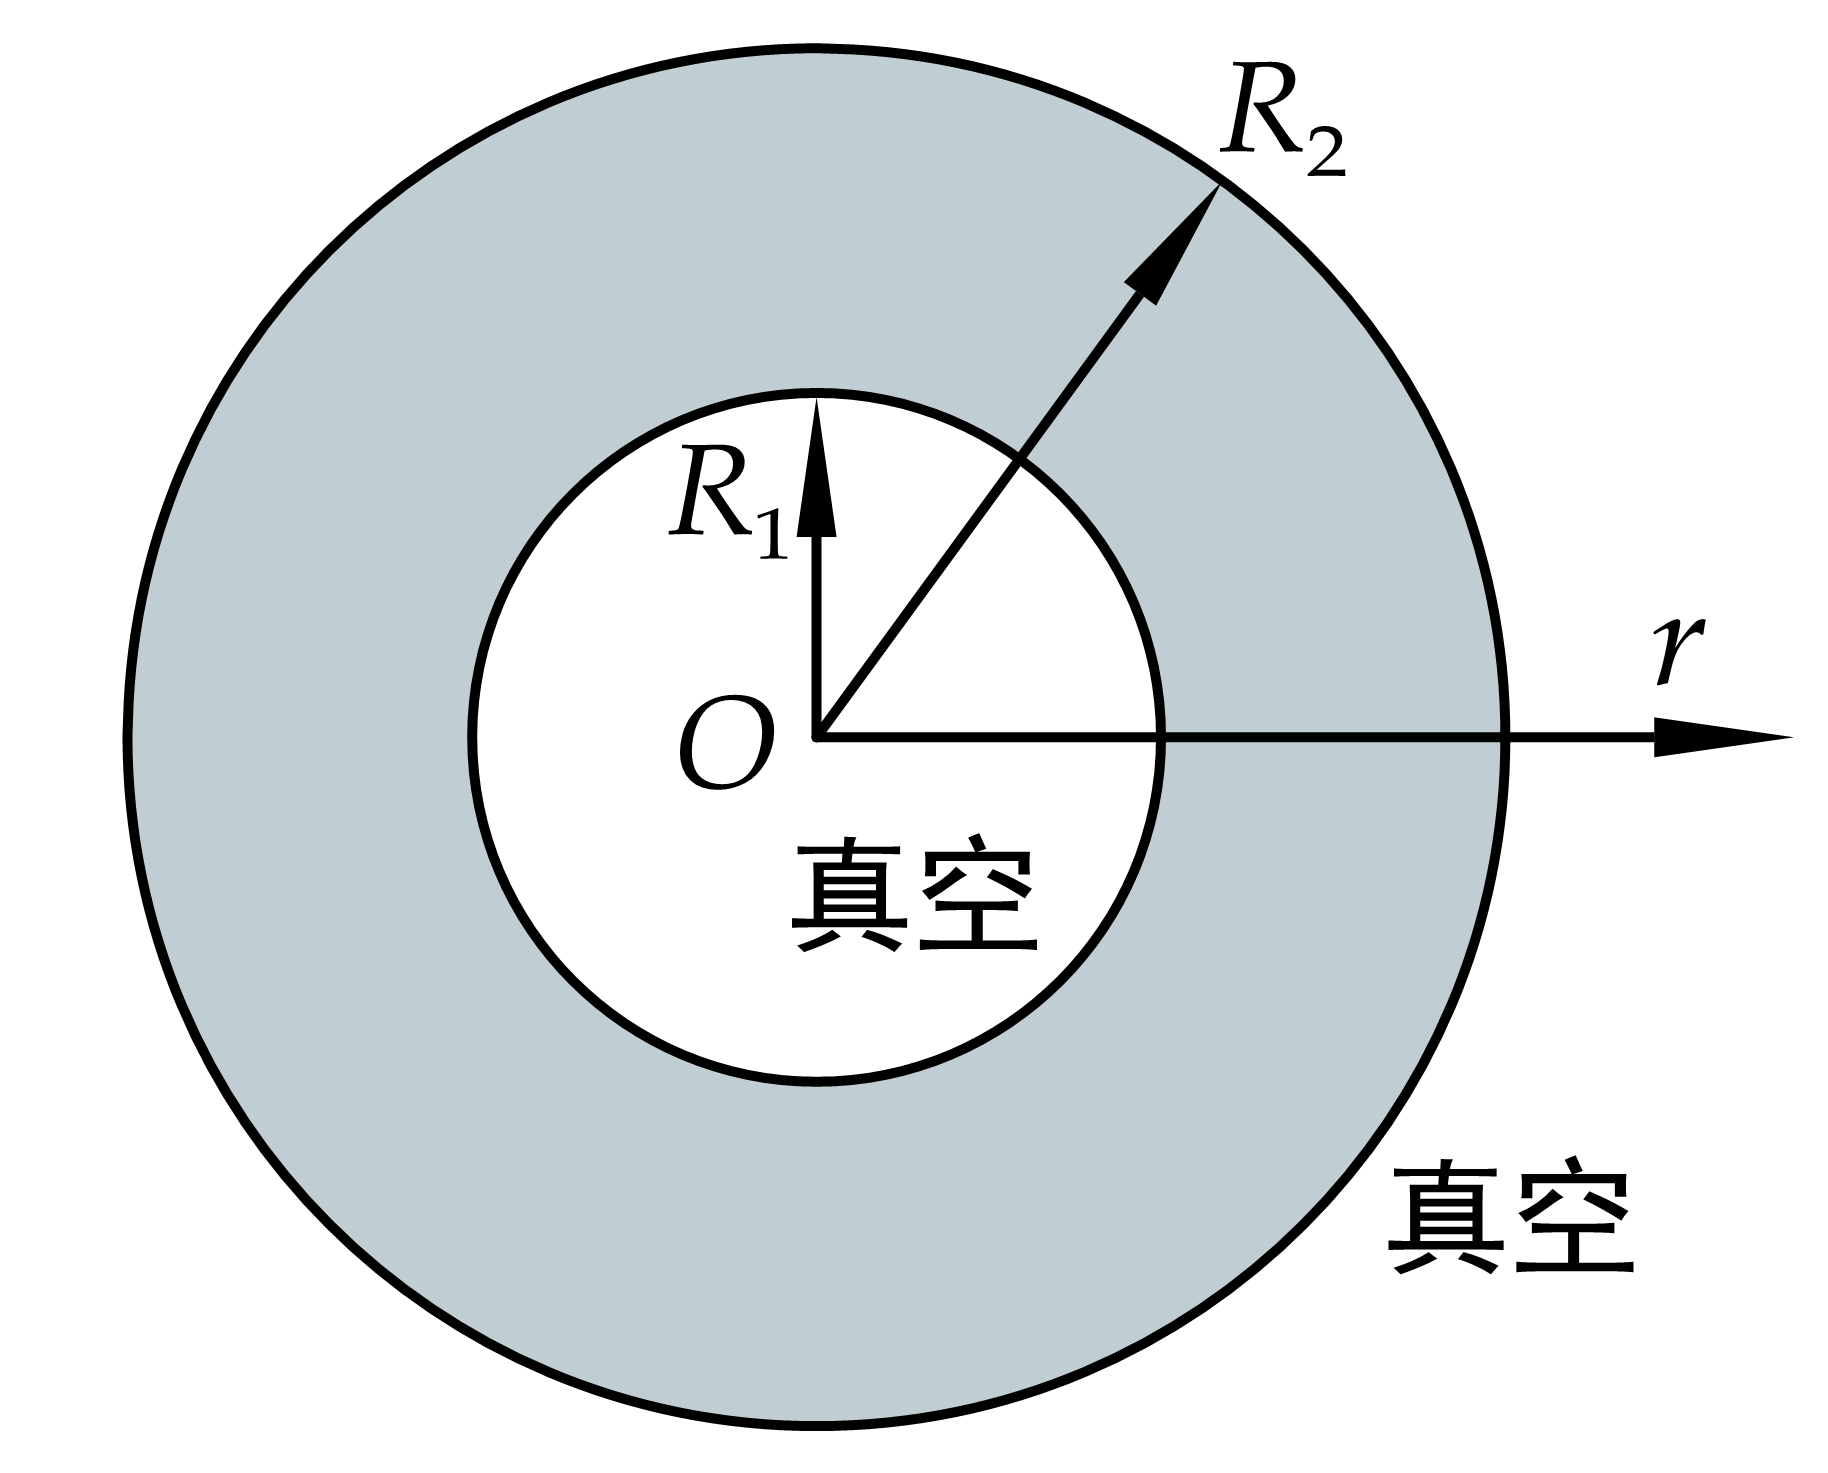
\includegraphics[scale=1]{figures/fig4.8.png}
        \end{figure}
        以球心为坐标原点建立一维球坐标系,如图所示,则临界时单能中子稳态扩散方程(增殖)为
        \begin{equation*}
            \ddv{\phi(r)}{r} + \frac{2}{r} \dv{\phi(r)}{r} + \frac{k_{\infty} - 1}{L^2}\phi(r) = 0 \xrightarrow{B^2 = (k_{\infty} - 1)/L^2} \ddv{\phi(r)}{r} + \frac{2}{r} \dv{\phi(r)}{r} + B^2 \phi(r) = 0,\,r > 0
        \end{equation*}
        通解为
        \begin{equation*}
            \phi(r) = A\frac{\nsin Br}{r} + C\frac{\ncos Br}{r}
        \end{equation*}
        
        边界条件
        \begin{enumerate}[(1)]
            \item $\lim\limits_{r\to R_1} J = 0$
            \begin{equation*}
                \lim_{r\to R_1} J = \lim_{r\to R_1} -D\dv{\phi(r)}{r} = \lim_{r\to R_1} -D\left(AB\frac{\ncos Br}{r} - A\frac{\nsin Br}{r^2} - BC\frac{\nsin Br}{r} - C\frac{\ncos Br}{r^2}\right) = 0
            \end{equation*}
            而$D \neq 0$,立即推
            \begin{equation*}
                AB\frac{\ncos BR_1}{R_1} - A\frac{\nsin BR_1}{R_1^2} - BC\frac{\nsin BR_1}{R_1} - C\frac{\ncos BR_1}{R_1^2} = 0
            \end{equation*}
            解得
            \begin{equation*}
                C = A\frac{BR_1 - \ntan BR_1}{BR_1 \ntan BR_1 + 1}
            \end{equation*}
            \item $\phi(R_2) = 0$
            \begin{equation*}
                \phi(R_2) = A\frac{\nsin BR_2}{R_2} + C\frac{\ncos BR_2}{R_2} = 0 \Rightarrow C = -A\ntan BR_2
            \end{equation*}
        \end{enumerate}
        联立可得
        \begin{equation*}
            \ntan BR_2 = \frac{\ntan BR_1 - BR_1}{BR_1\ntan BR_1 + 1}
        \end{equation*}
    \end{solution}
\end{exercise}

\begin{exercise}
    一维无限平板几何下,坐标原点左侧和右侧分别为两种非增殖但含中子源的材料,两种材料的扩散系数相同、中子扩散长度的倒数分别为$\kappa_{\symrm{l}}^2$和$\kappa_{\symrm{r}}^2$,相应的中子源强分别为$\kappa_{\symrm{l}}^2 \vPhi_{\symrm{l}}$和$\kappa_{\symrm{r}}^2 \vPhi_{\symrm{r}}$。
    \begin{enumerate}[(1)]
        \item 试计算该一维无限平板内的中子注量率分布和原点处的中子注量率;
        \item 试画出区间$[-5/\kappa_{\symrm{l}},\,5/\kappa_{\symrm{r}}]$内在$\vPhi_{\symrm{l}}=0,\,\vPhi_{\symrm{r}}=1,\,\kappa_{\symrm{l}}=\kappa_{\symrm{r}}=\kappa$时的中子注量率分布;
        \item 试画出区间$[-5/\kappa_{\symrm{l}},\,5/\kappa_{\symrm{r}}]$内在$\vPhi_{\symrm{l}}=2,\,\vPhi_{\symrm{r}}=1,\,\kappa_{\symrm{l}}=3\kappa,\,\kappa_{\symrm{r}}=\kappa$时的中子注量率分布。
    \end{enumerate}
    \begin{solution}
        \begin{enumerate}[(1)]
            \item 如图所示,以$x>0$为例,有
            \begin{figure}[H]
                \centering
                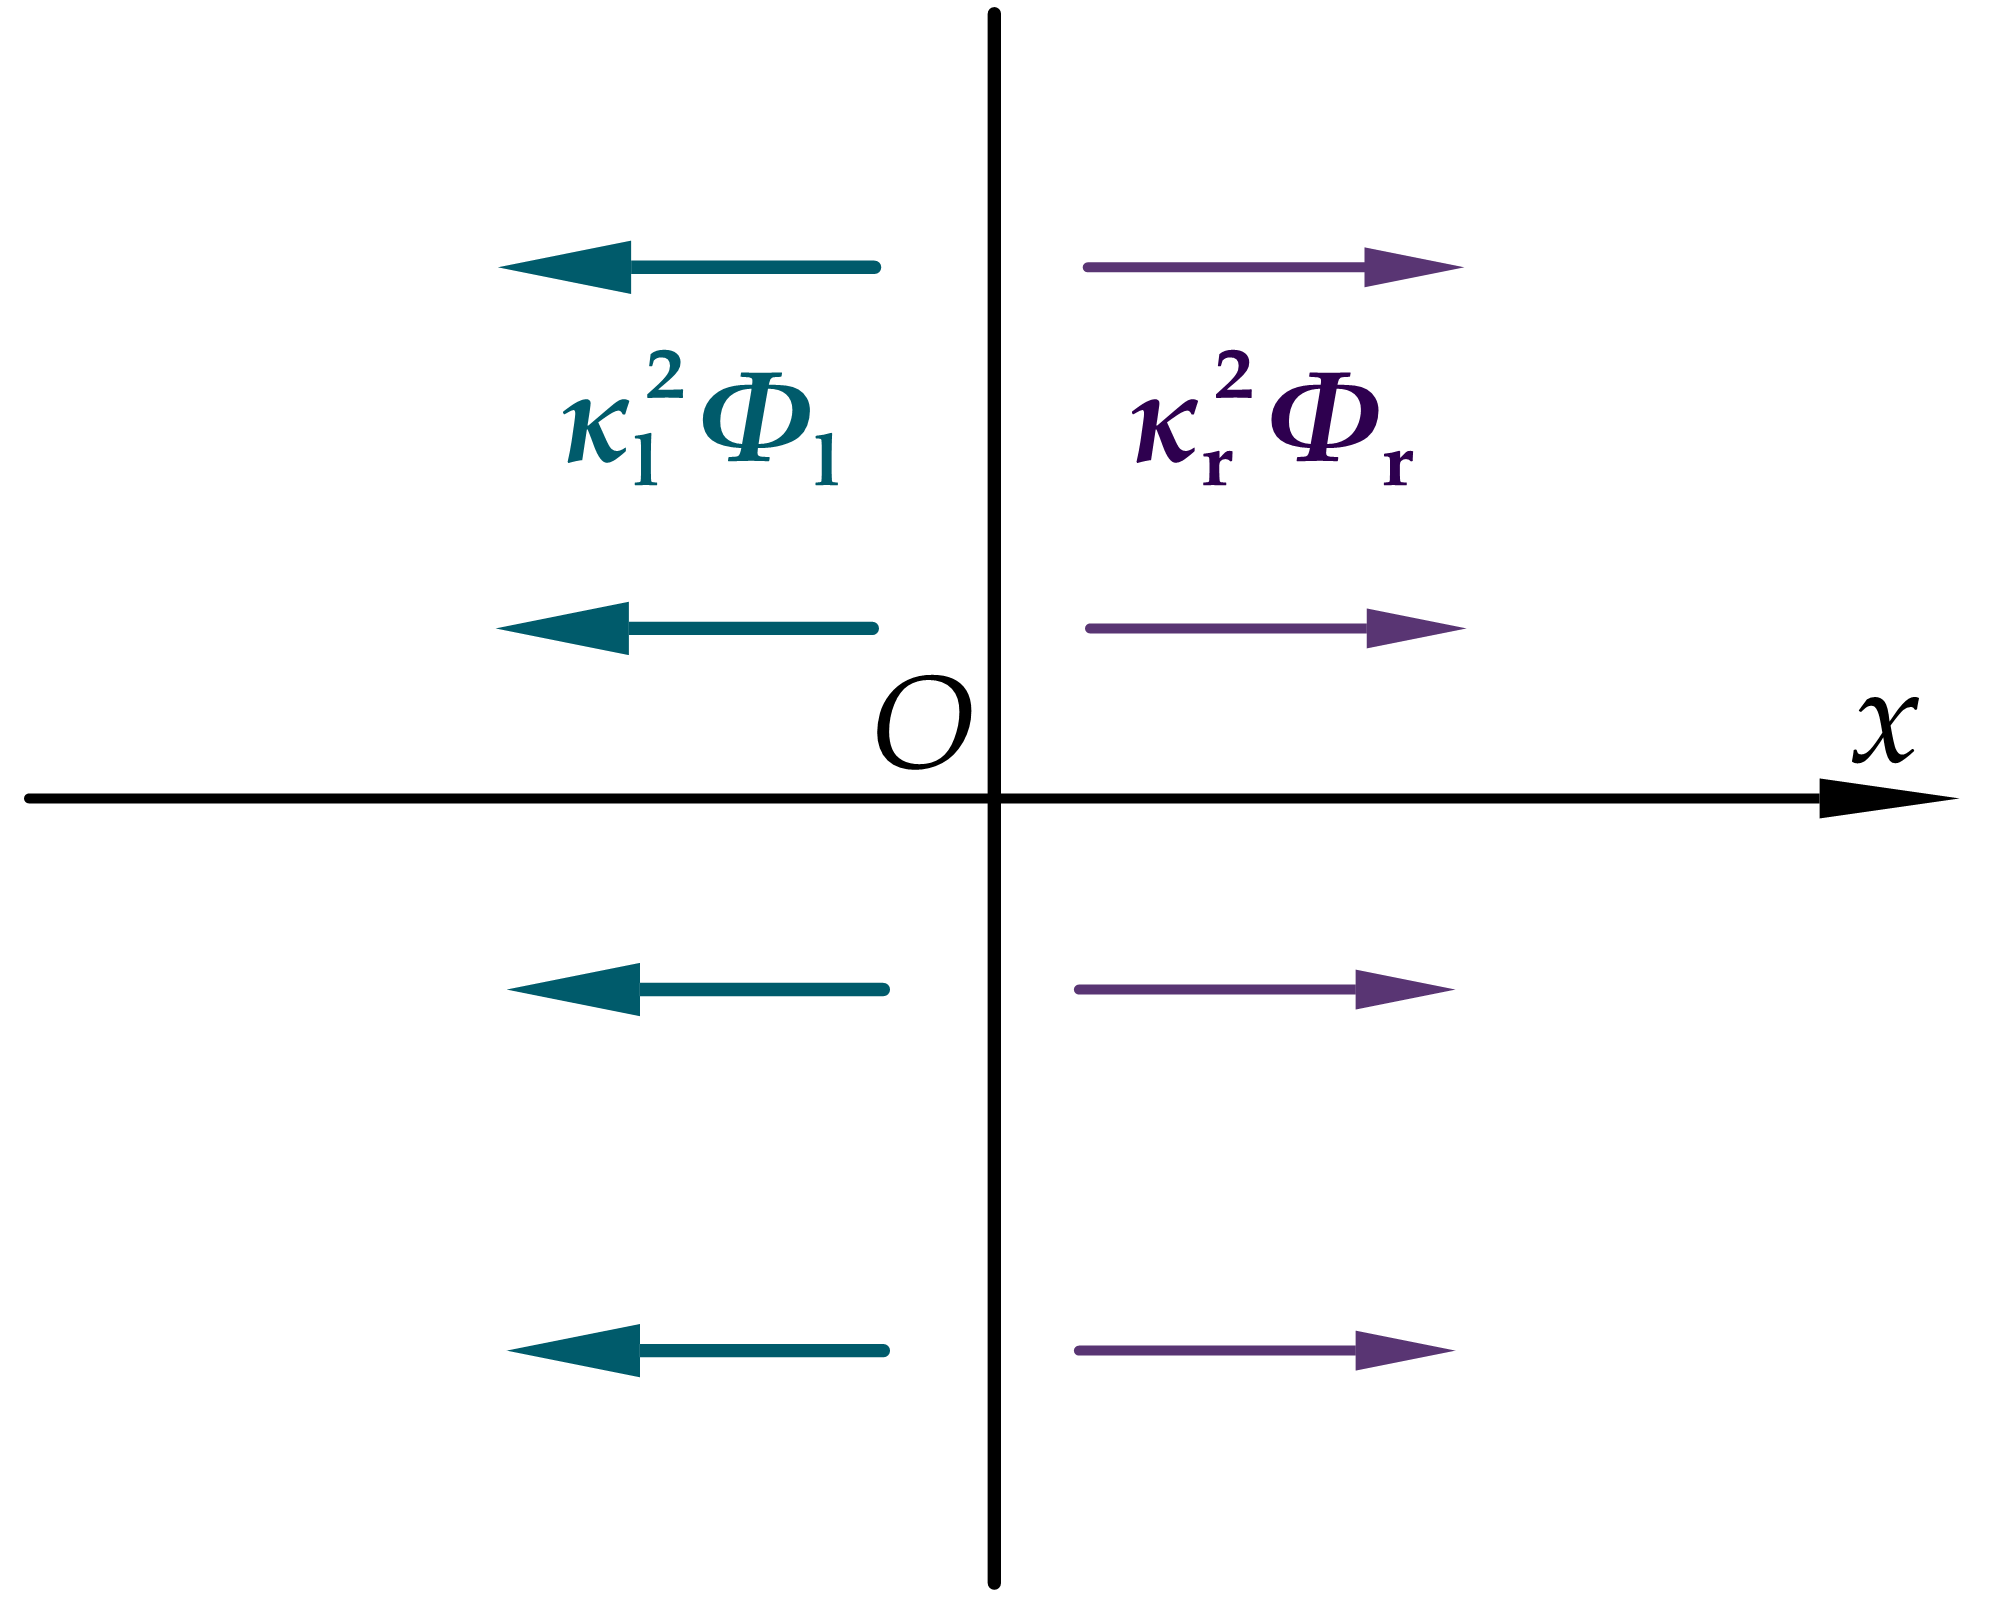
\includegraphics[scale=1]{figures/fig4.9.png}
            \end{figure}
            \begin{equation*}
                \ddv{\phi_{\symrm{r}}(x)}{x} - \frac{\phi_{\symrm{r}}(x)}{L^2} = 0,\,x > 0
            \end{equation*}
            通解为
            \begin{equation*}
                \phi_{\symrm{r}}(x) = A_{\symrm{r}} \symrm{e}^{-x/L_r} + C_{\symrm{r}} \symrm{e}^{x/L_r}
            \end{equation*}
            边界条件
            \begin{enumerate}[(a)]
                \item $\phi_{\symrm{r}}(x)$为有限正值,于是$C_{\symrm{r}} = 0$;
                \item $\lim\limits_{x\to 0^{+}} J_{\symrm{r}}(x) = \kappa_{\symrm{r}}^2 \vPhi_{\symrm{r}} \Rightarrow A_{\symrm{r}} = \frac{\kappa_{\symrm{r}}^2 \vPhi_{\symrm{r}} L_{\symrm{r}}}{D} \xlongequal[\kappa_{\symrm{r}}^2 L_{\symrm{r}}^2 = 1]{\kappa_{\symrm{r}} L_{\symrm{r}} = 1} \frac{\kappa_{\symrm{r}} \vPhi_{\symrm{r}}}{D}$
            \end{enumerate}
            于是
            \begin{equation*}
                \phi_{\symrm{r}}(x) = \frac{\kappa_{\symrm{r}} \vPhi_{\symrm{r}}}{D} \symrm{e}^{-\kappa_{\symrm{r}}x},\,x\geqslant 0
            \end{equation*}
            同理
            \begin{equation*}
                \phi_{\symrm{l}}(x) = \frac{\kappa_{\symrm{l}} \vPhi_{\symrm{l}}}{D} \symrm{e}^{\kappa_{\symrm{l}}x},\,x < 0
            \end{equation*}
            即
            \begin{equation*}
                \phi(x) = \begin{cases}
                    \frac{\kappa_{\symrm{l}} \vPhi_{\symrm{l}}}{D} \symrm{e}^{\kappa_{\symrm{l}}x},\,x < 0 \\
                    \frac{\kappa_{\symrm{r}} \vPhi_{\symrm{r}}}{D} \symrm{e}^{-\kappa_{\symrm{r}}x},\,x > 0
                \end{cases}
            \end{equation*}
            原点处中子注量率不连续,有
            \begin{align*}
                &\phi(0^{-}) = \lim_{x \to 0} \phi_{\symrm{l}}(x) = \lim_{x \to 0} \frac{\kappa_{\symrm{l}} \vPhi_{\symrm{l}}}{D} \symrm{e}^{\kappa_{\symrm{l}}x} = \frac{\kappa_{\symrm{l}} \vPhi_{\symrm{l}}}{D} \\
                &\phi(0^{+}) = \lim_{x \to 0} \phi_{\symrm{r}}(x) = \lim_{x \to 0} \frac{\kappa_{\symrm{r}} \vPhi_{\symrm{r}}}{D} \symrm{e}^{-\kappa_{\symrm{r}}x} = \frac{\kappa_{\symrm{r}} \vPhi_{\symrm{r}}}{D}
            \end{align*}
            \item 由题意,此时
            \begin{equation*}
                \phi(x) = \begin{cases}
                    \phi_{\symrm{l}}(x) = 0,\,x < 0 \\
                    \phi_{\symrm{r}}(x) = \frac{\kappa}{D} \symrm{e}^{-\kappa x},\,x > 0
                \end{cases}
            \end{equation*}
            \begin{figure}[H]
                \centering
                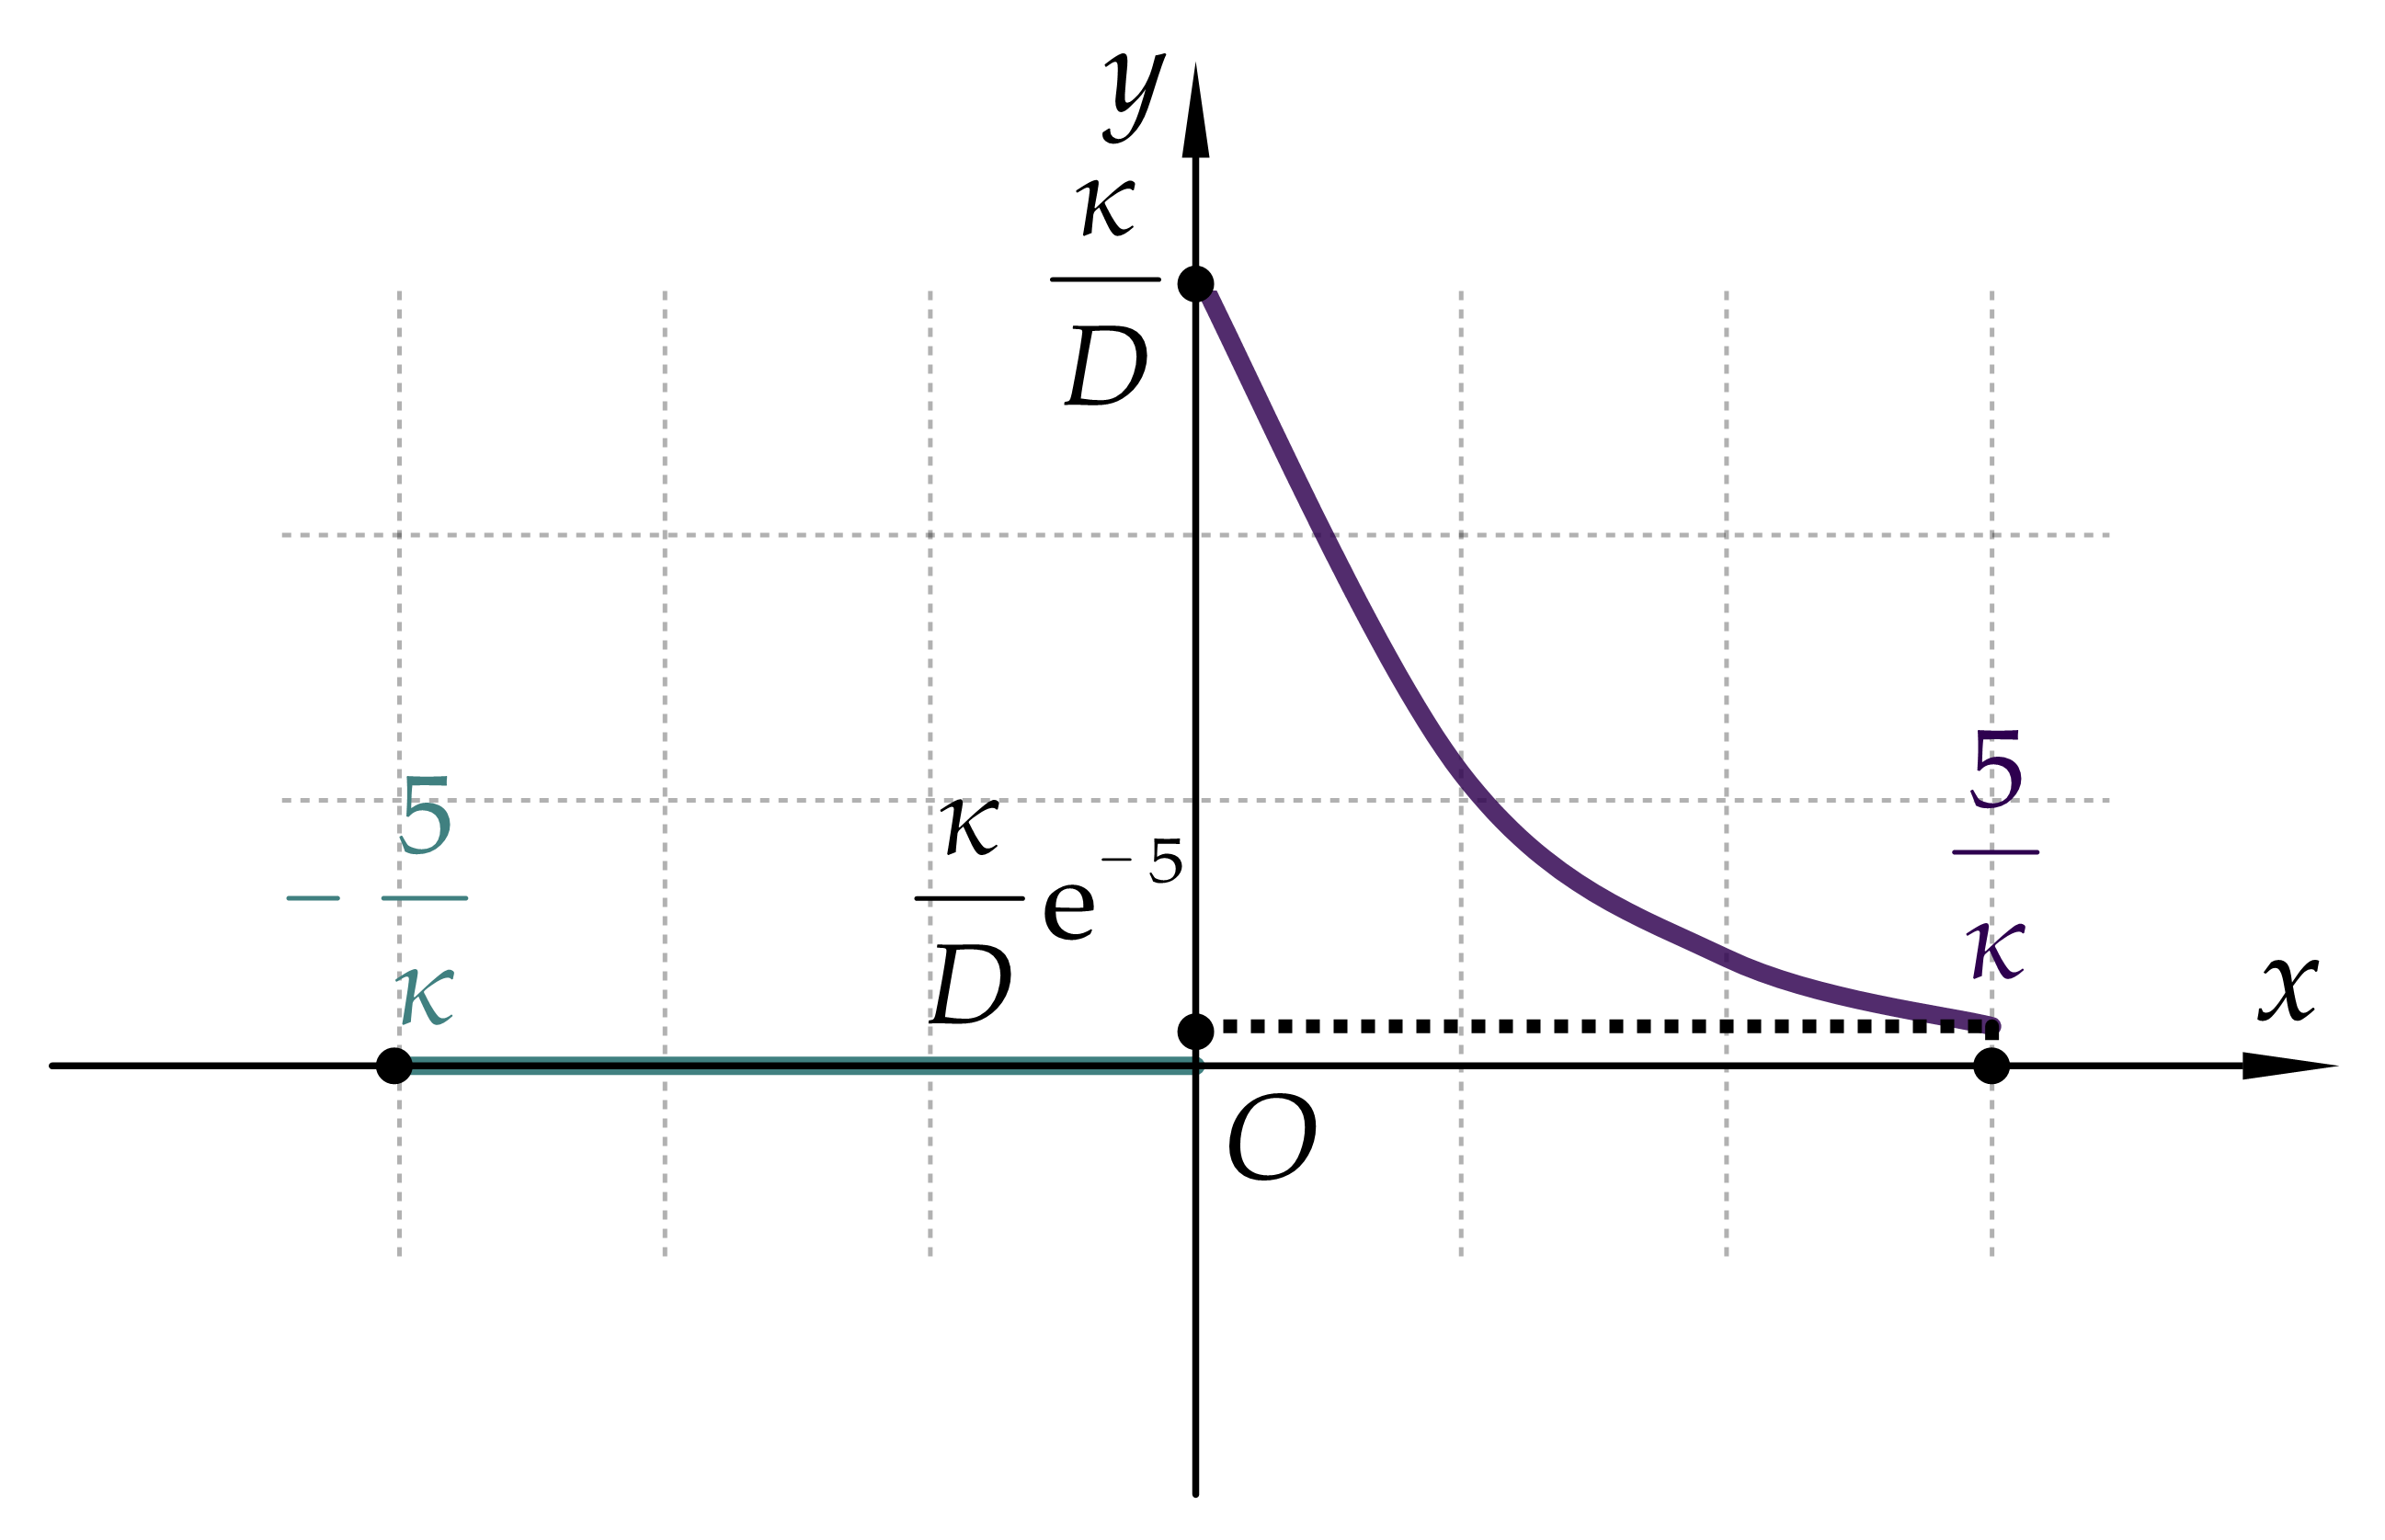
\includegraphics[scale=1]{figures/fig4.9-2.png}
            \end{figure}
            \item 由题意,此时
            \begin{equation*}
                \phi(x) = \begin{cases}
                    \phi_{\symrm{l}}(x) = \frac{6\kappa}{D} \symrm{e}^{3\kappa x},\,x < 0 \\
                    \phi_{\symrm{r}}(x) = \frac{\kappa}{D} \symrm{e}^{-\kappa x},\,x > 0
                \end{cases}
            \end{equation*}
            \begin{figure}[H]
                \centering
                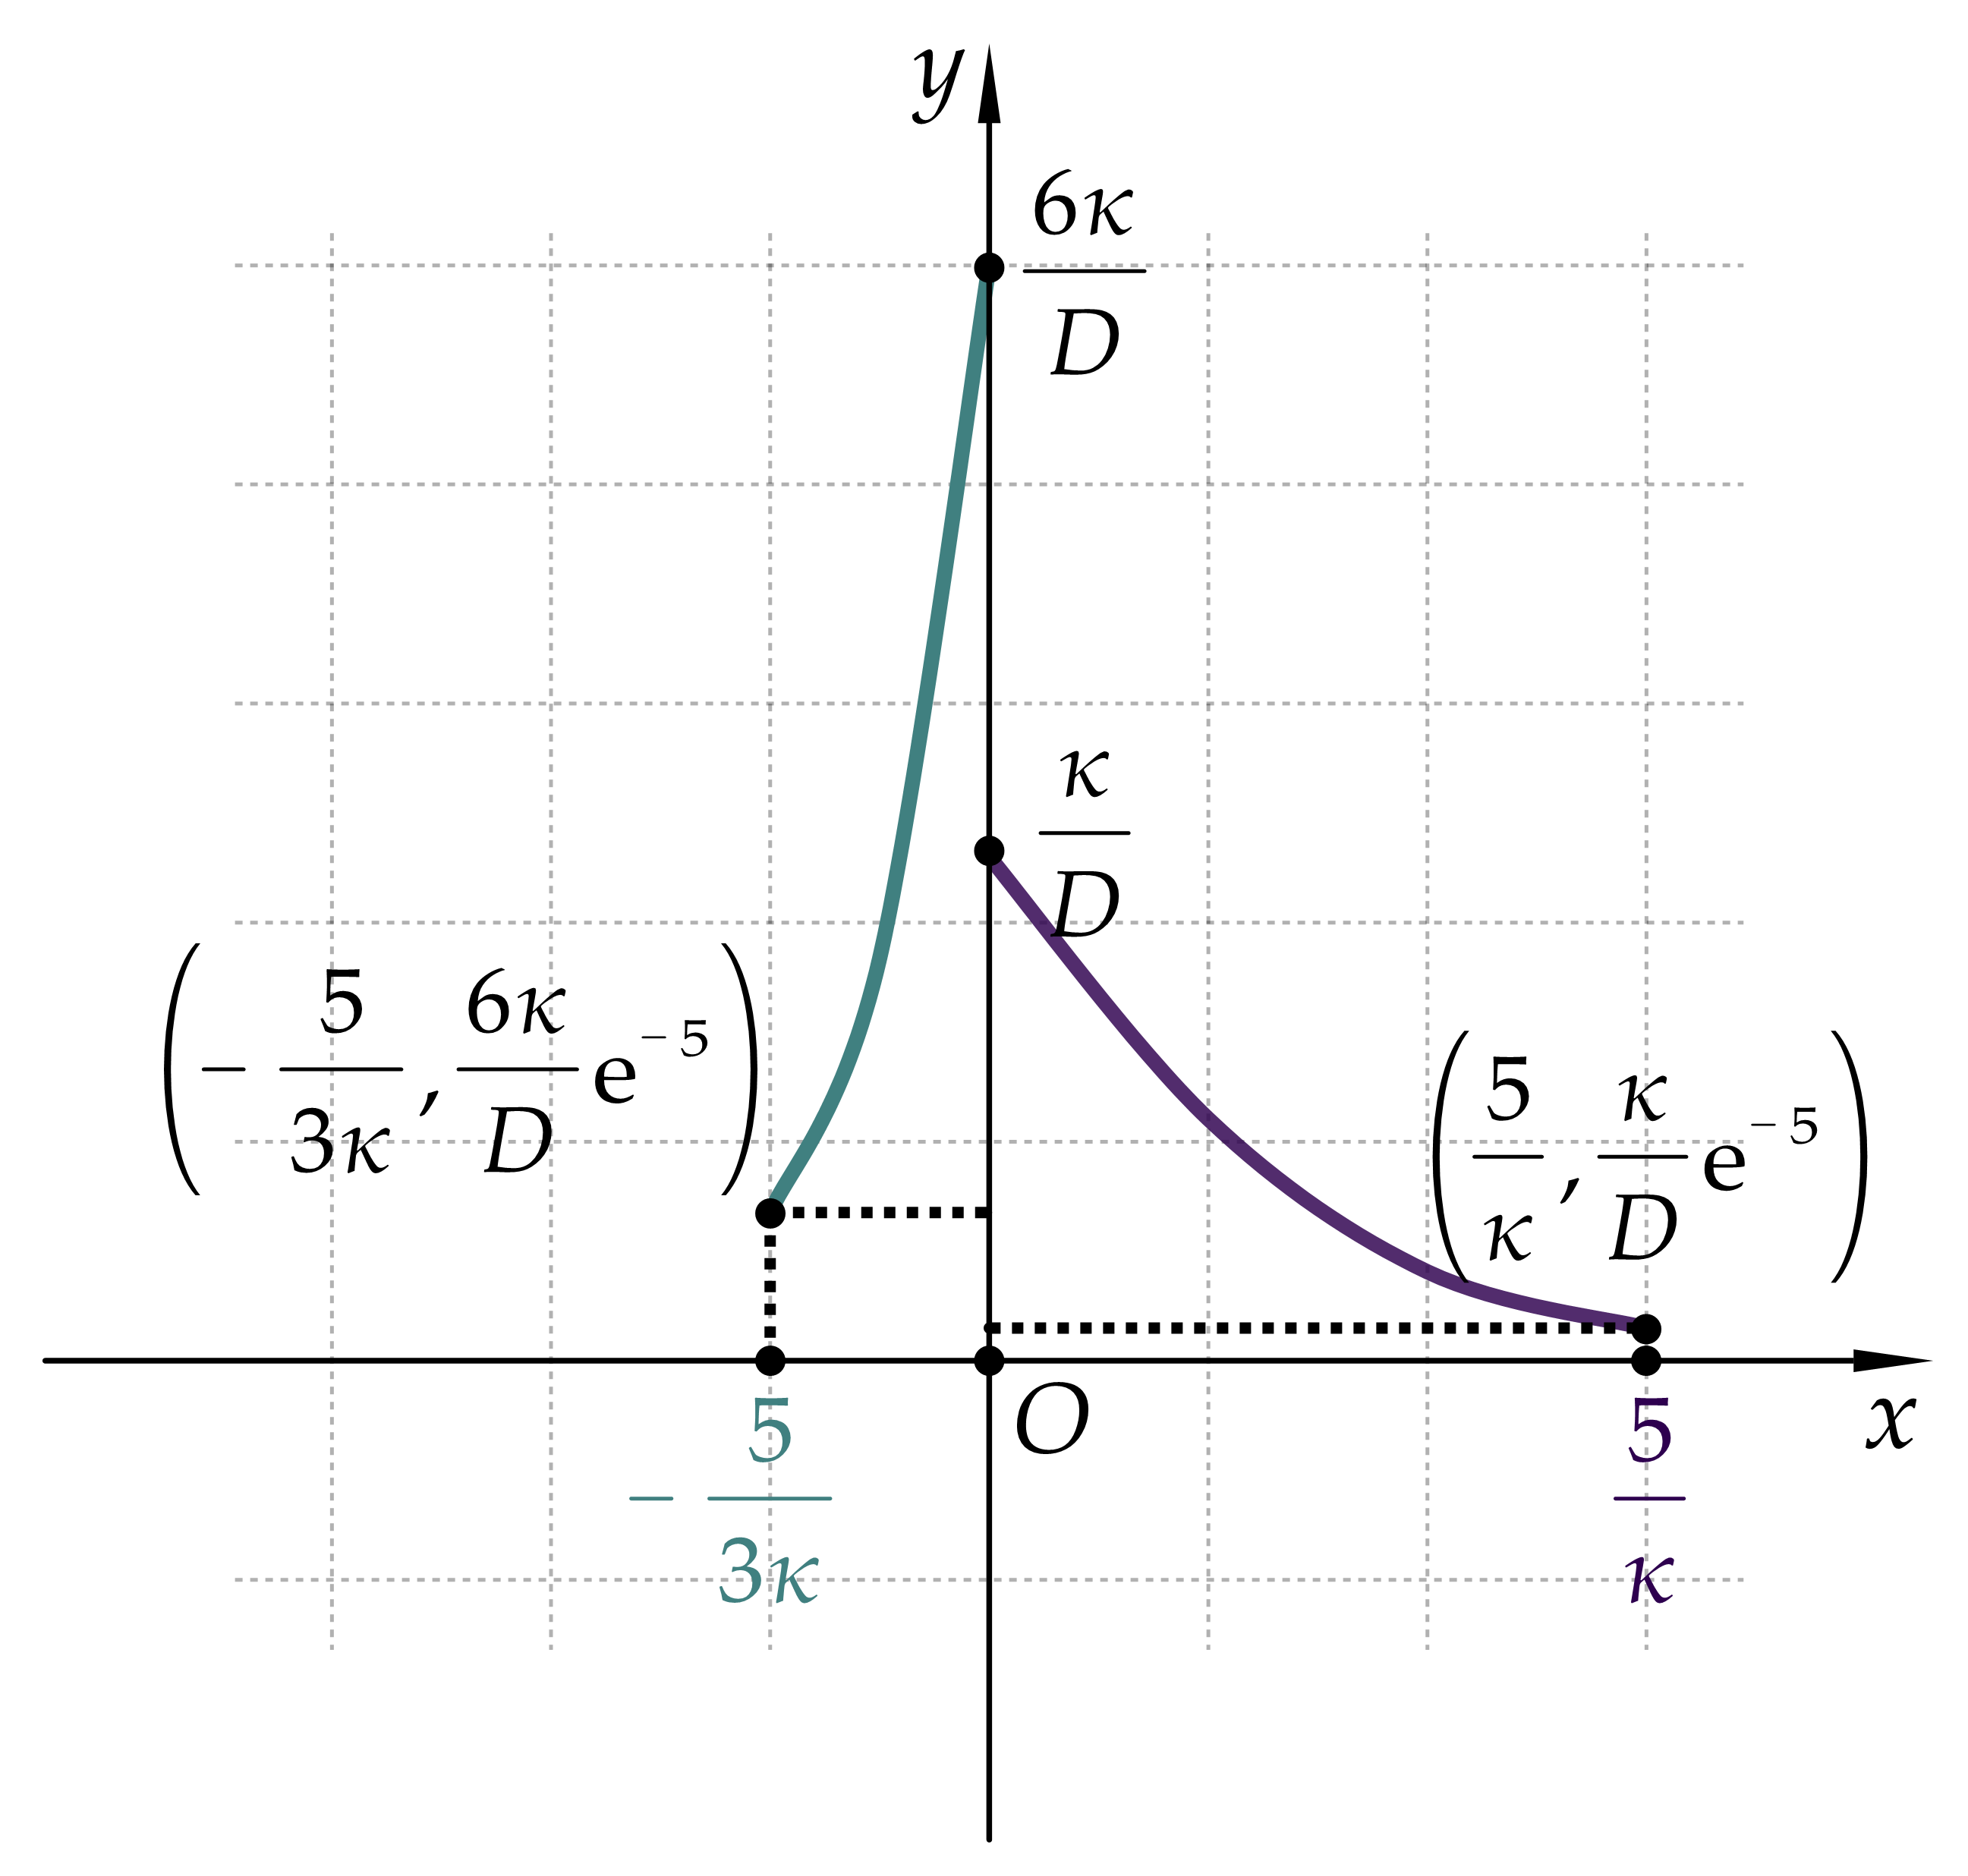
\includegraphics[scale=0.8]{figures/fig4.9-3.png}
            \end{figure}
        \end{enumerate}
    \end{solution}
\end{exercise}

\chapter{中子能谱与群常数计算}
\section*{习题}

\begin{exercise}
    名词解释:\,中子能谱,\,慢化密度.\,
    \begin{solution}
        \begin{enumerate}[(1)]
            \item 中子能谱:\,中子注量率随中子能量的分布函数,\,用$\phi(E)$表示;\,
            \item 慢化密度:\,单位时间单位体积内慢化到能量$E$以下的中子数,\,用$q(E)$表示.\,
        \end{enumerate}
    \end{solution}
\end{exercise}

\begin{exercise}
    请简单描述压水堆中的中子能谱.\,
    \begin{solution}
        \begin{figure}[H]
            \centering
            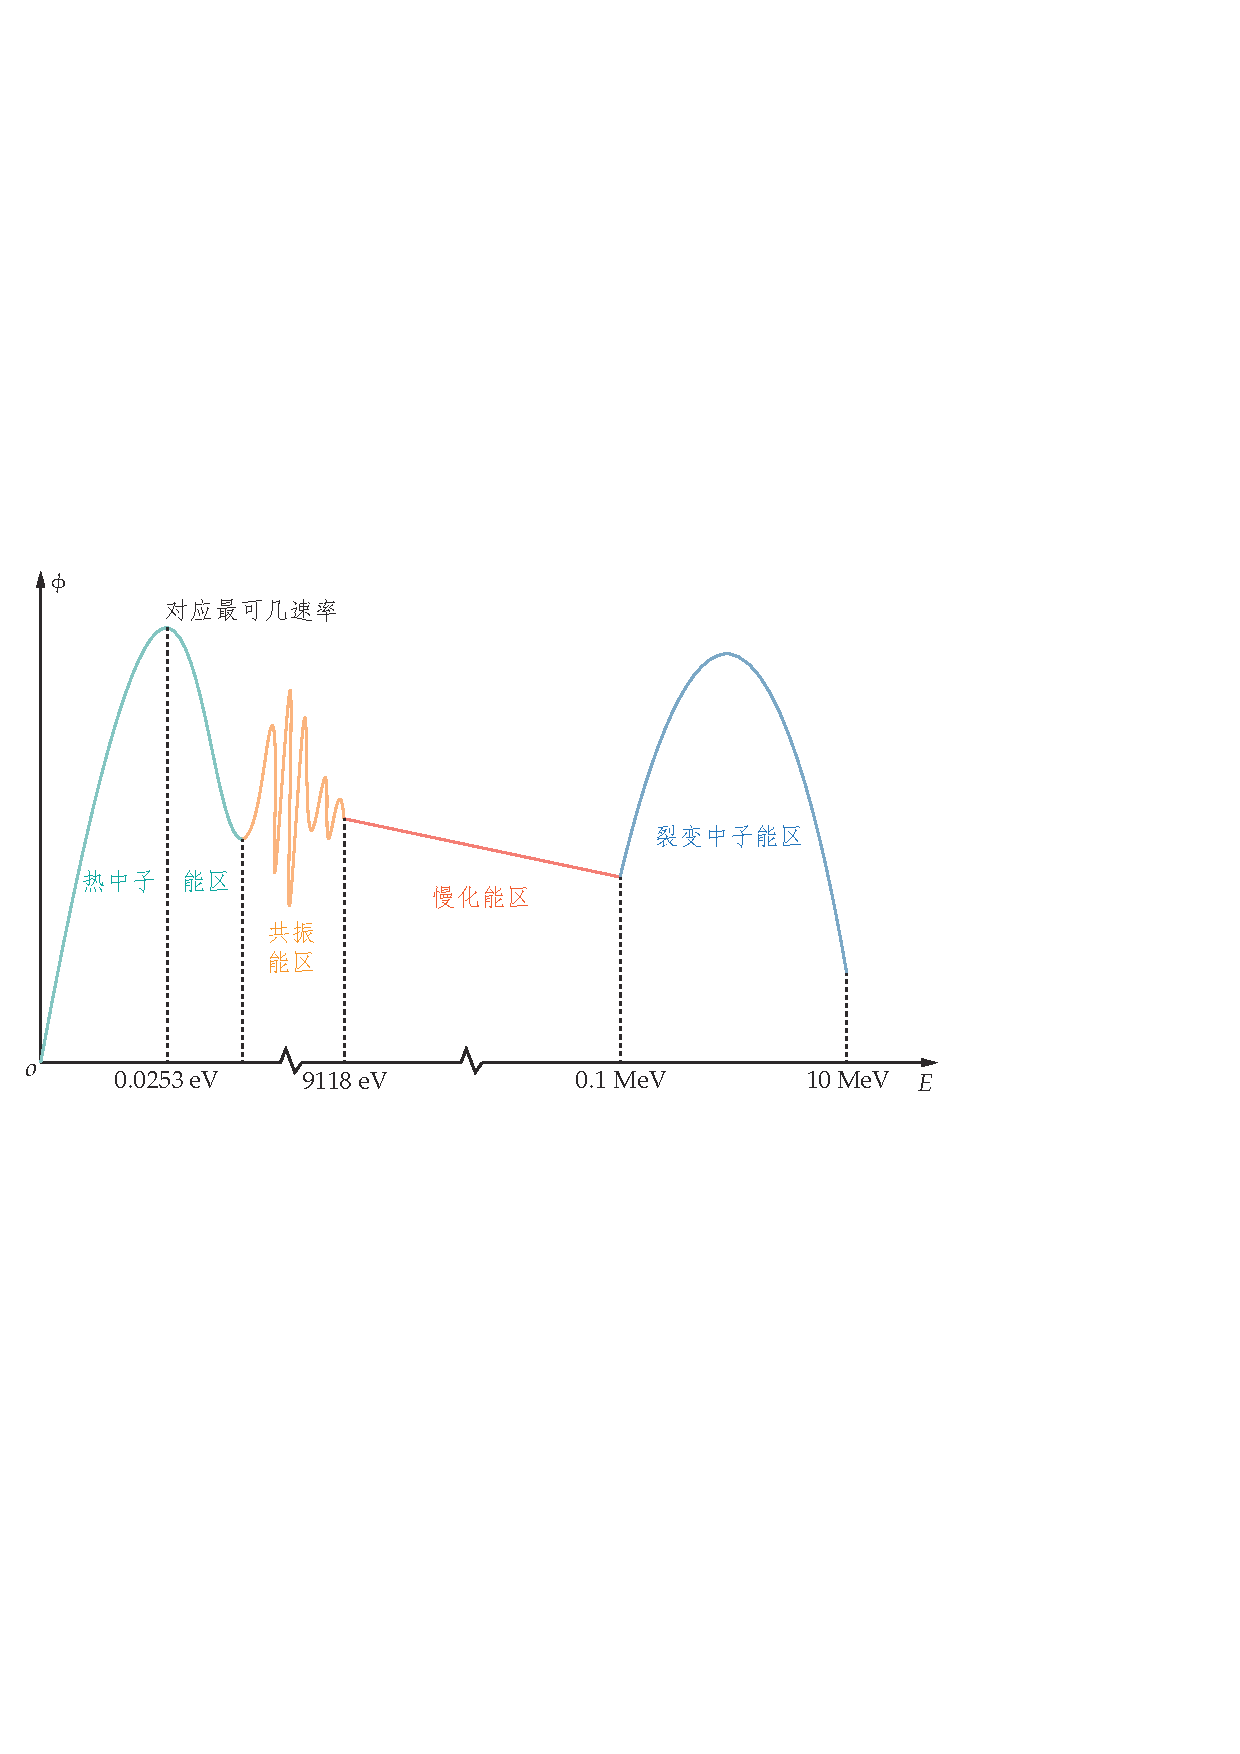
\includegraphics[scale=0.6]{figures/fig5.1.pdf}
        \end{figure}
        \begin{enumerate}[(1)]
            \item 0.1 MeV \textasciitilde \, 10 MeV:\,裂变中子能谱,\,包括瞬发中子和缓发中子;\,
            \item 9118 eV \textasciitilde \, 0.1 MeV:\,慢化能区\,近似用直线描述平均作用,\,1/E谱或费米谱;\,
            \item 共振能区:\,共振能谱;\,
            \item 热中子能区:\,麦克斯韦谱,\,$E=0.0253\,\symrm{MeV}$对应中子最可几速率.\,
        \end{enumerate}
    \end{solution}
\end{exercise}

\begin{exercise}
    什么是首次飞行逃脱概率?\,什么是丹可夫效应?\,
    \begin{solution}
        \begin{enumerate}[(1)]
            \item 首次飞行逃脱概率:\,在燃料芯块内产生的均匀和各向同性分布的,\,能量为$E$的中子未经碰撞逃出芯块在慢化剂内发生首次碰撞的概率,\,用$P_0(E)$表示;\,
            \item 丹可夫效应:\,中子逸出燃料芯块后不一定在慢化剂中发生下一次碰撞,\,也有可能在相邻燃料芯块中发生碰撞,\,这种相邻燃料棒间的相互影响称为丹可夫效应.\,
        \end{enumerate}
    \end{solution}
\end{exercise}

\begin{exercise}
    试列出至少四种共振计算方法.\,
    \begin{solution}
        \begin{enumerate}[(1)]
            \item 等价原理;
            \item 广义等价方法;
            \item 子群方法;
            \item 超细群方法;
            \item 小波展开法.
        \end{enumerate}
    \end{solution}
\end{exercise}

\begin{exercise}
    什么是能量自屏效应和空间自屏效应?\,
    \begin{solution}
        \begin{enumerate}[(1)]
            \item 能量自屏效应:\,共振峰附近的中子吸收截面极大,\,中子接近共振峰会被吸收,\,无法继续慢化到内部,\,内部能量处中子注量率低,\,相当于因为能量的原因,\,使共振峰内部被屏蔽;\,
            \item 空间自屏效应:\,超热中子在慢化剂中产生,\,则慢化剂中超热中子更多,\,且由于燃料棒中${}^{238}\symrm{U}$对超热中子具有很强的共振吸收,\,使得慢化剂中产生的超热中子刚进入到燃料表面就被吸收,\,超热中子几乎没有机会进入燃料棒内部,\,即燃料外层对内层有屏蔽作用.\,
        \end{enumerate}
    \end{solution}
\end{exercise}

\begin{exercise}
    压水堆中栅格的非均匀效应会影响到四因子模型中的哪些参数?\,作用机制是什么?\,
    \begin{solution}
        \begin{equation*}
            k_{\infty} = \highlight{NavyBlue}{\color{black} $\varepsilon$} {\color{NavyBlue!40} \uparrow} \highlight{Bittersweet}{\color{black} $p$} {\color{Bittersweet!40} \uparrow \uparrow} \highlight{xkcdHunterGreen} {\color{black} $f$} {\color{xkcdHunterGreen!40} \downarrow} \eta
        \end{equation*}
        \begin{enumerate}[(1)]
            \item 快中子在燃料棒内裂变产生,\,其在燃料块中分布高于慢化剂中,\,将增加${}^{238}\symrm{U}$裂变可能性,\,则快中子倍增系数\highlight{NavyBlue}{\color{black} $\varepsilon$}\,{\color{NavyBlue!40} $\uparrow$};
            \item 由于空间自屏效应的存在,\,超热中子几乎没有机会进入燃料棒内部,\,则燃料棒内部对超热中子的共振吸收减少,\,逃脱共振吸收概率\highlight{Bittersweet}{\color{black} $p$} {\color{Bittersweet!40} $\uparrow$};
            \item 经过充分慢化,\,中子能量可能越过共振吸收段,\,逃脱共振吸收概率\highlight{Bittersweet}{\color{black} $p$} {\color{Bittersweet!40} $\uparrow$};
            \item 热中子在慢化剂中产生,\,其在慢化剂中分布高于燃料棒中,\,燃料吸收热中子的概率减小,\,热中子利用系数\highlight{xkcdHunterGreen} {\color{black} $f$} {\color{xkcdHunterGreen!40} $\downarrow$}.
        \end{enumerate}
    \end{solution}
\end{exercise}

\begin{exercise}
    什么是过慢化和欠慢化?\,
    \begin{solution}
        \begin{enumerate}[(1)]
            \item 过慢化:\,$k_{\infty}$最大值对应的水-铀比右侧为过慢化区,\,这里慢化剂偏多,\,中子完全慢化;\,
            \item 欠慢化:\,$k_{\infty}$最大值对应的水-铀比左侧为欠慢化区,\,这里慢化剂偏少,\,中子未完全慢化.\,
        \end{enumerate}
    \end{solution}
\end{exercise}

\chapter{燃耗与中毒}
\section*{习题}

\begin{exercise}
    名词解释:\,燃耗深度,\,堆芯寿期,\,饱和裂变产物,\,非饱和裂变产物,\,裂变产物中毒,\,剩余反应性.\,
    \begin{solution}
        \begin{enumerate}[(1)]
            \item 燃耗深度:\,装入堆芯的单位质量燃料所发出的能量,\,单位是MWd/tU.\,
            \item 堆芯寿期:\,核反应堆装料后从开始运行直到堆芯$\keff$降到1时满功率运行时间.\,
            \item 饱和裂变产物:\,裂变产物由于自身吸收中子或衰变会消失,\,到一定时间后其消失与产生达到平衡.\,
            \item 非饱和裂变产物:\,裂变产物一直不会消失或消失几乎为零,\,随着核反应堆的运行其浓度不断增加积累.\,
            \item 裂变产物中毒:\,毒物(在热中子能区具有很大中子吸收截面的裂变产物)吸收中子导致的反应性亏损.\,
            \item 剩余反应性:\,核反应堆没有控制毒物时的反应性.\,
        \end{enumerate}
    \end{solution}
\end{exercise}

\begin{exercise}
    试写出核反应堆中的燃耗方程,\,并给出每一项的物理意义.\,
    \begin{solution}
        \begin{enumerate}[(1)]
            \item 假设A为重同位素,\,有
            
            \vspace{1em}
            \begin{minipage}{0.1\columnwidth}
                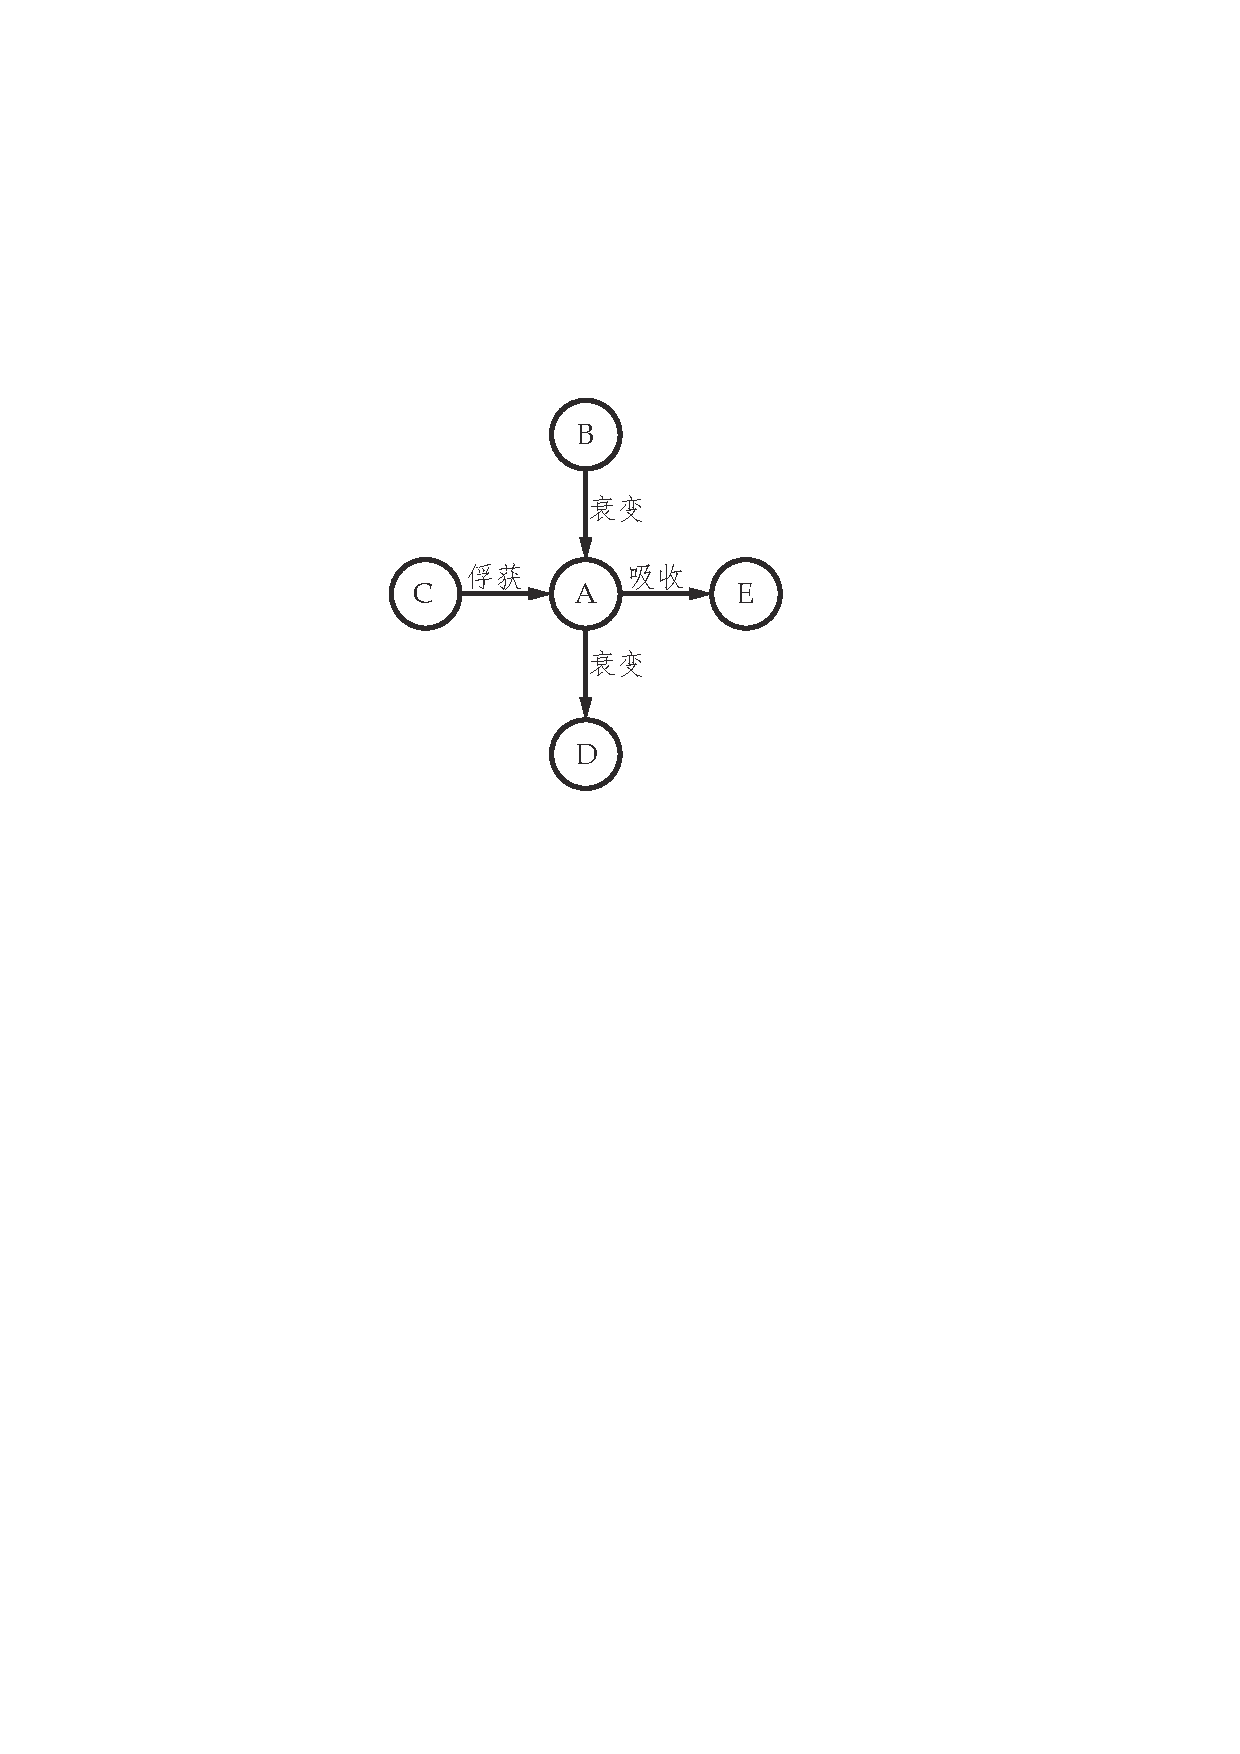
\includegraphics[scale=0.6]{figures/fig6.1.pdf}
            \end{minipage}
            \hfil
            \begin{minipage}{0.85\columnwidth}
                \begin{equation*}
                    \tikzmarknode{N}{\highlight{red}{$\dv{N_{\symrm{A}}(t)}{t}$}} =
                    \color{BlueViolet}
                    \overbrace{
                        \left(\tikzmarknode{C}{\highlight{Plum}{\color{black} $N_{\symrm{C}} \sigma_{\gamma,\,\symrm{C}} \phi$}} {\color{black} +} \tikzmarknode{B}{\highlight{NavyBlue}{\color{black}  $\lambda_{\symrm{B}} N_{\symrm{B}}$}}\right)
                    }^{\text{\fangsong \footnotesize \textcolor{BlueViolet!85}{核素A产生率}}}
                        \color{black} - 
                    \color{RawSienna}
                        \overbrace{
                        \left(\tikzmarknode{A1}{\highlight{Bittersweet}{\color{black} $N_{\symrm{A}} \sigma_{\symrm{a,\,A}} \phi$}} {\color{black} +} \tikzmarknode{A2}{\highlight{xkcdHunterGreen}{\color{black}   $\lambda_{\symrm{A}} N_{\symrm{A}}$}}\right)
                    }^{\text{\fangsong \footnotesize \textcolor{RawSienna!85}{核素A消失率}}}
                \end{equation*}
                \vspace*{0.5\baselineskip}
                \begin{tikzpicture}[overlay,remember picture,>=stealth,nodes={align=left,inner ysep=1pt},<-]
                    % 核素A变化率
                    \path (N.north) ++ (0,0.5em) node[anchor=south east,color=Maroon!85] (Ntext){\fangsong{\footnotesize 核素A变化率}};
                    \draw [color=Maroon](N.north) |- ([xshift=-0.3ex,color=Maroon]Ntext.south west);
                    % 核素C俘获中子产生A
                    \path (C.north) ++ (-3.2,-1.8em) node[anchor=north west,color=Plum!85] (Ctext){{\fangsong{\footnotesize 核素C俘获中子产生A}}};
                    \draw [color=Plum](C.south) |- ([xshift=-0.3ex,color=Plum]Ctext.south west);
                    % 核素B衰变产生A
                    \path (B.north) ++ (-2.6,-3.2em) node[anchor=north west,color=NavyBlue!85] (Btext){{\fangsong{\footnotesize 核素B衰变产生A}}};
                    \draw [color=NavyBlue](B.south) |- ([xshift=-0.3ex,color=NavyBlue]Btext.south west);
                    % 核素A吸收中子(裂变或俘获)消失
                    \path (A1.north) ++ (0.1,-3.2em) node[anchor=north west,color=Bittersweet!85] (A1text){\fangsong{\footnotesize 核素A吸收中子(裂变或俘获)消失}};
                    \draw [color=Bittersweet](A1.south) |- ([xshift=-0.3ex,color=Bittersweet]A1text.south east);
                    % 核素A衰变消失
                    \path (A2.north) ++ (0.1,-1.8em) node[anchor=north west,color=xkcdHunterGreen!85] (A2text){\fangsong{\footnotesize 核素A衰变消失}};
                    \draw [color=xkcdHunterGreen](A2.south) |- ([xshift=-0.3ex,color=xkcdHunterGreen]A2text.south east);
                \end{tikzpicture}
            \end{minipage}

            \vspace{1em}

            \item 假设a为中等质量核素或轻核素,\,有
            
            \vspace{1em}
            \begin{minipage}{0.1\columnwidth}
                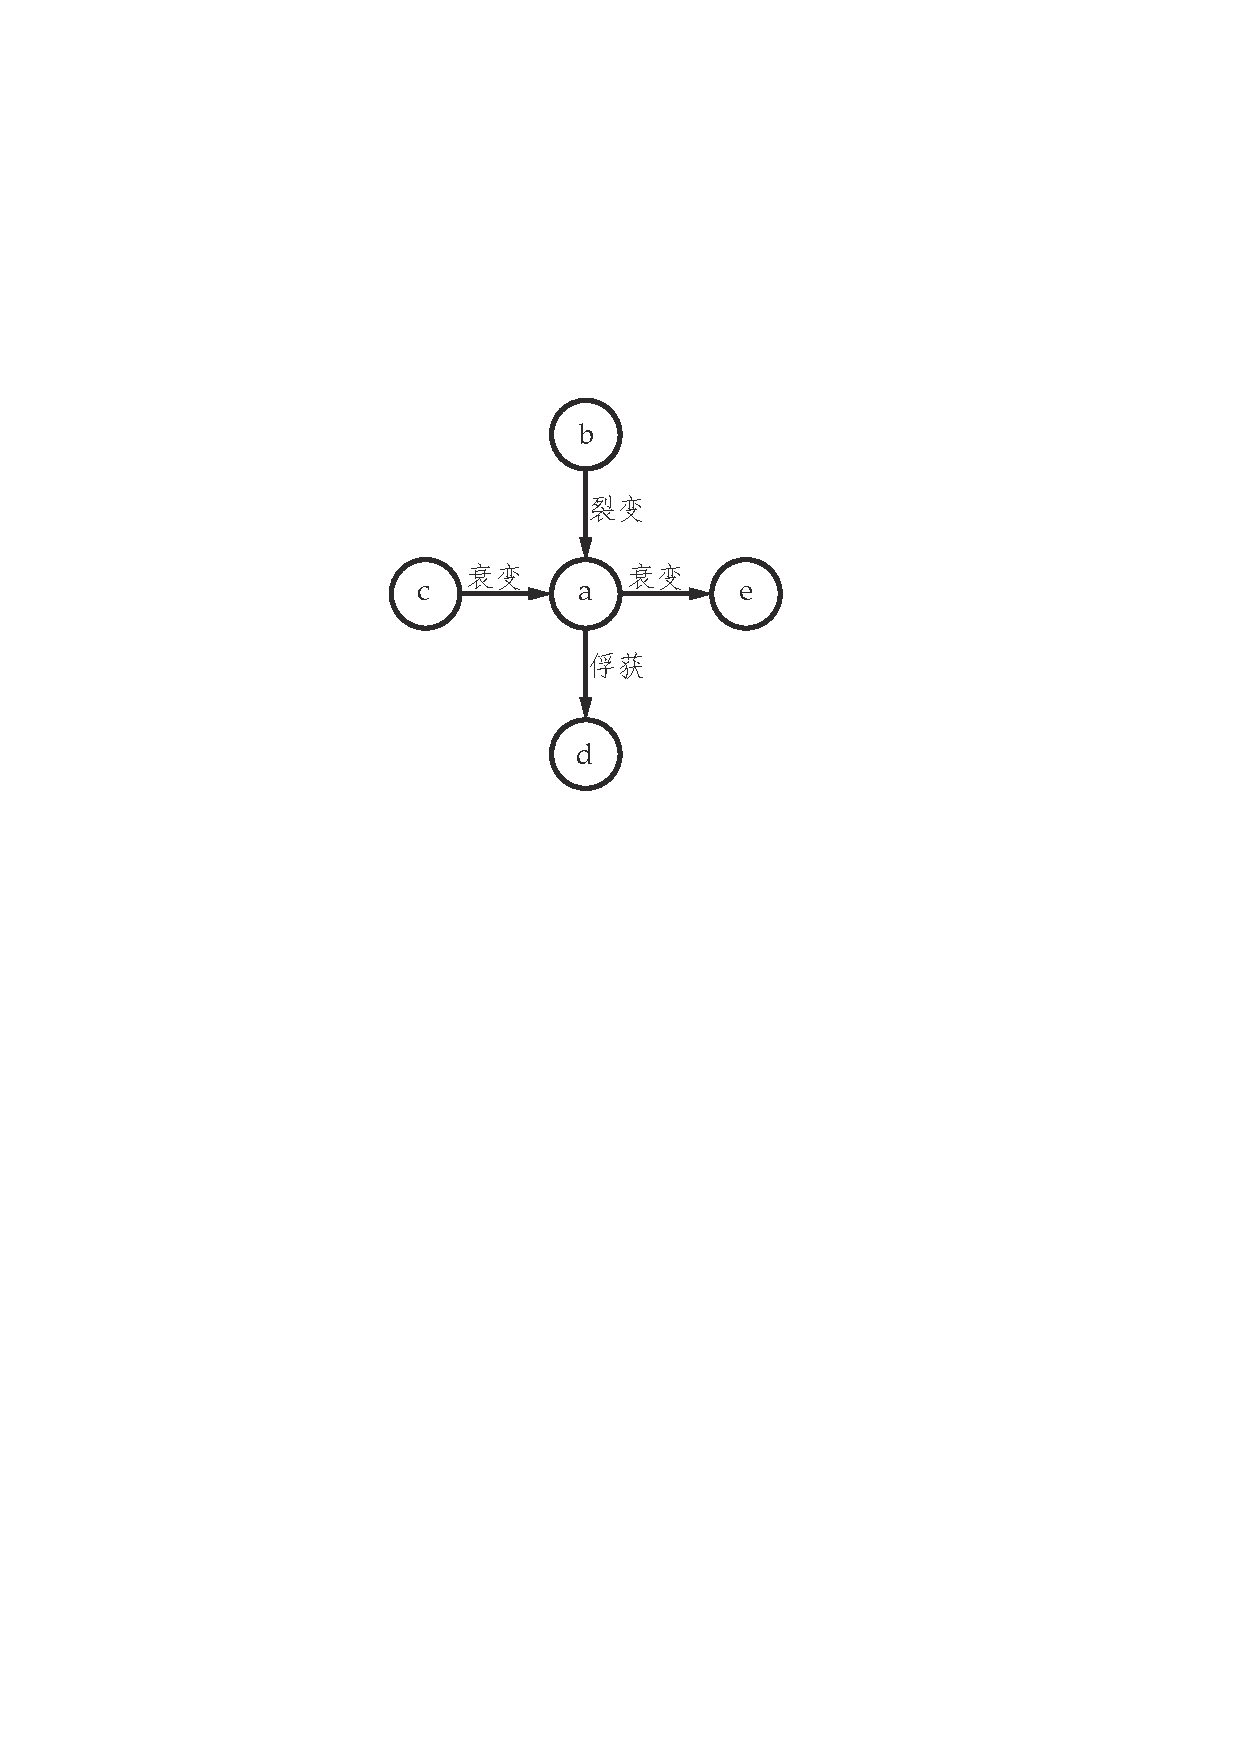
\includegraphics[scale=0.6]{figures/fig6.2.pdf}
            \end{minipage}
            \hfil
            \begin{minipage}{0.85\columnwidth}
                \begin{equation*}
                    \tikzmarknode{N}{\highlight{red}{$\dv{N_{\symrm{a}}(t)}{t}$}} =
                    \color{BlueViolet}
                    \overbrace{
                        \left(\tikzmarknode{C}{\highlight{Plum}{\color{black} $\gamma_{\symrm{a}} \vSigma_{\symrm{f}} \phi$}} {\color{black} +} \tikzmarknode{B}{\highlight{NavyBlue}{\color{black}  $\lambda_{\symrm{c}} N_{\symrm{c}}$}}\right)
                    }^{\text{\fangsong \footnotesize \textcolor{BlueViolet!85}{核素a产生率}}}
                        \color{black} - 
                    \color{RawSienna}
                        \overbrace{
                        \left(\tikzmarknode{A1}{\highlight{Bittersweet}{\color{black} $N_{\symrm{a}} \sigma_{\gamma,\,\symrm{a}} \phi$}} {\color{black} +} \tikzmarknode{A2}{\highlight{xkcdHunterGreen}{\color{black}   $\lambda_{\symrm{a}} N_{\symrm{a}}$}}\right)
                    }^{\text{\fangsong \footnotesize \textcolor{RawSienna!85}{核素a消失率}}}
                \end{equation*}
                \vspace*{0.5\baselineskip}
                \begin{tikzpicture}[overlay,remember picture,>=stealth,nodes={align=left,inner ysep=1pt},<-]
                    % 核素a变化率
                    \path (N.north) ++ (0,0.5em) node[anchor=south east,color=Maroon!85] (Ntext){\fangsong{\footnotesize 核素a变化率}};
                    \draw [color=Maroon](N.north) |- ([xshift=-0.3ex,color=Maroon]Ntext.south west);
                    % 核素b裂变产生a
                    \path (C.north) ++ (-3.2,-1.8em) node[anchor=north west,color=Plum!85] (Ctext){{\fangsong{\footnotesize 核素b裂变产生a}}};
                    \draw [color=Plum](C.south) |- ([xshift=-0.3ex,color=Plum]Ctext.south west);
                    % 核素c衰变产生a
                    \path (B.north) ++ (-2.6,-3.2em) node[anchor=north west,color=NavyBlue!85] (Btext){{\fangsong{\footnotesize 核素c衰变产生a}}};
                    \draw [color=NavyBlue](B.south) |- ([xshift=-0.3ex,color=NavyBlue]Btext.south west);
                    % 核素a俘获中子消失
                    \path (A1.north) ++ (0.1,-3.2em) node[anchor=north west,color=Bittersweet!85] (A1text){\fangsong{\footnotesize 核素a俘获中子消失}};
                    \draw [color=Bittersweet](A1.south) |- ([xshift=-0.3ex,color=Bittersweet]A1text.south east);
                    % 核素a衰变消失
                    \path (A2.north) ++ (0.1,-1.8em) node[anchor=north west,color=xkcdHunterGreen!85] (A2text){\fangsong{\footnotesize 核素a衰变消失}};
                    \draw [color=xkcdHunterGreen](A2.south) |- ([xshift=-0.3ex,color=xkcdHunterGreen]A2text.south east);
                \end{tikzpicture}
            \end{minipage}
        \end{enumerate}
    \end{solution}
\end{exercise}

\begin{exercise}
    试阐述什么是预估-校正法及其实现过程.\,
    \begin{solution}
        \begin{figure}[H]
            \centering
            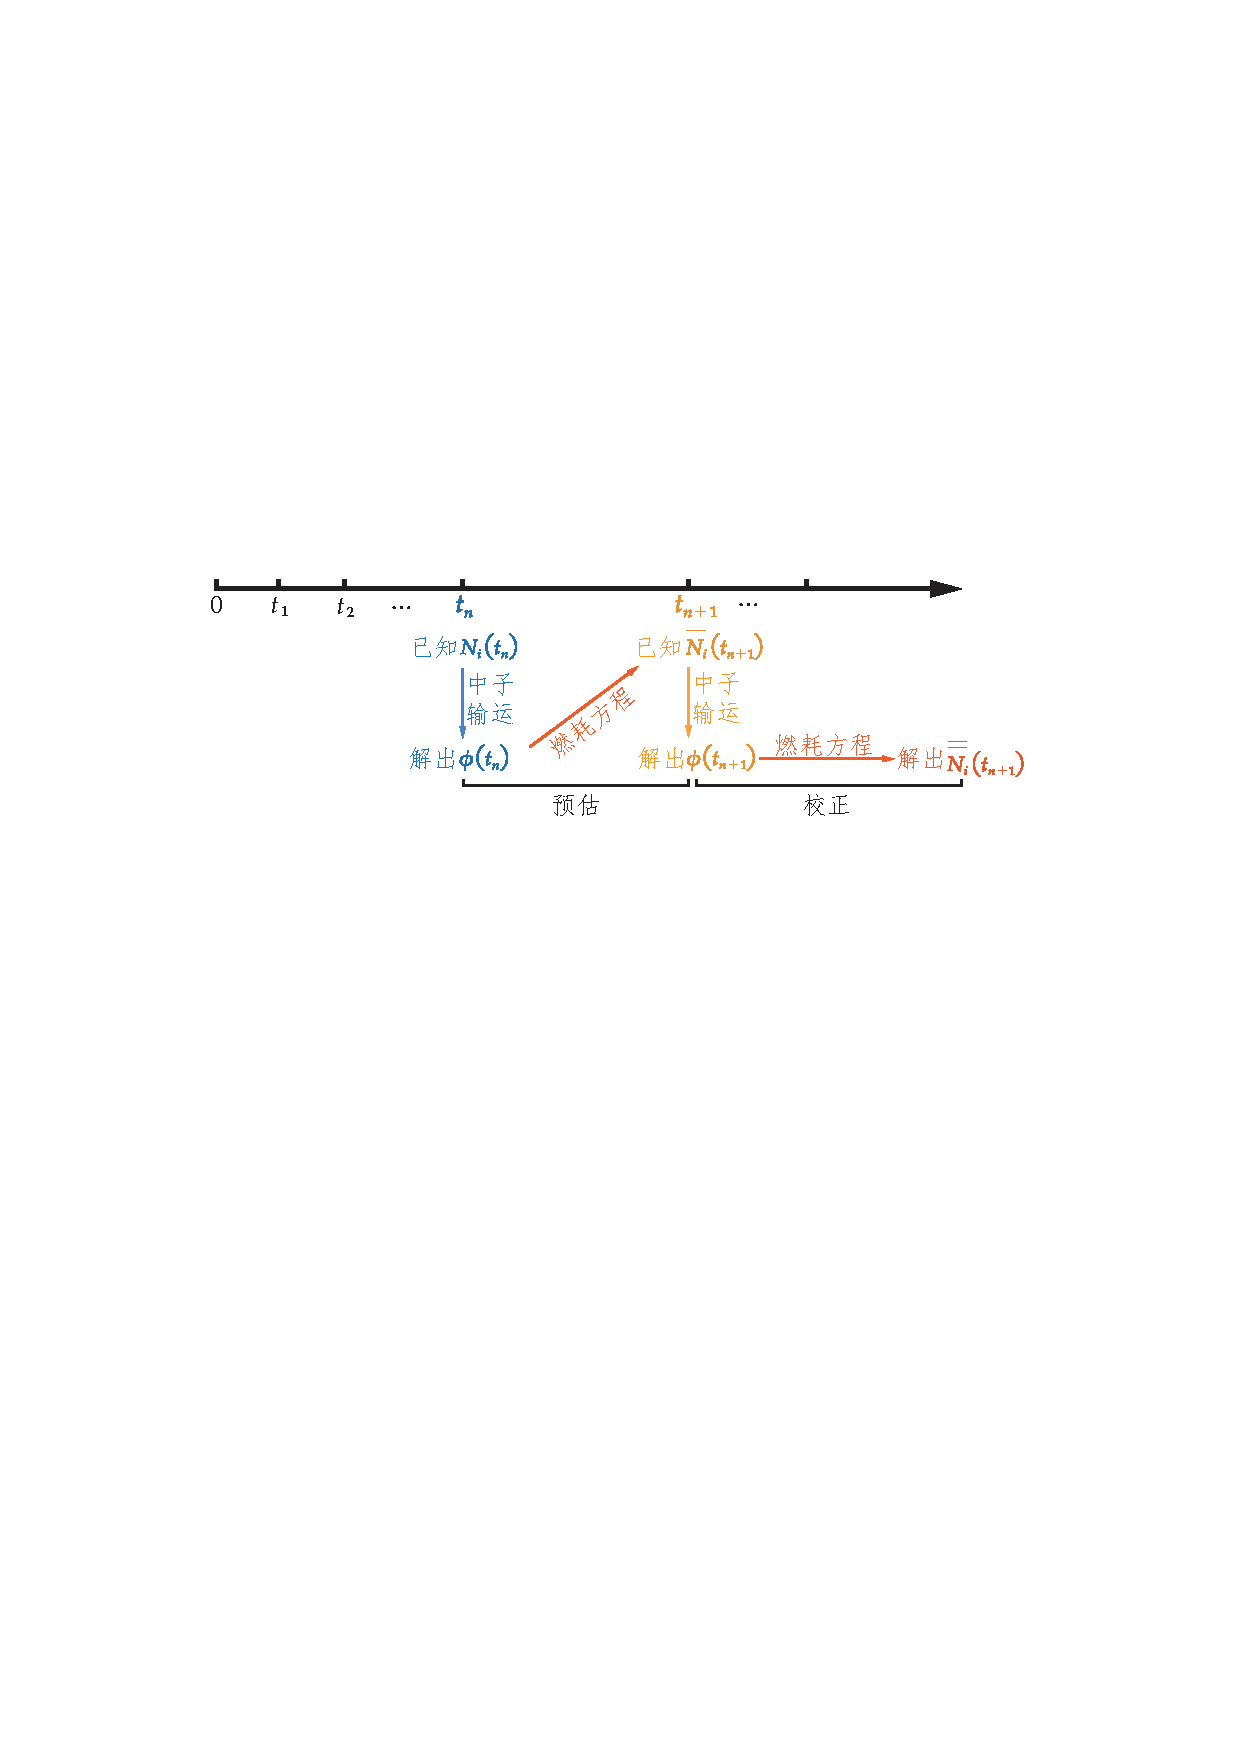
\includegraphics[scale=0.8]{figures/fig6.3.pdf}
        \end{figure}
    最后取
    \begin{equation*}
        N_i(t_{n+1}) = \frac{1}{2} \left[\overline{N_i}(t_{n+1}) + \overline{\overline{N_i}}(t_{n+1})\right]
    \end{equation*}
    \end{solution}
\end{exercise}

\begin{exercise}
    一座核反应堆,\,额定电功率为1200\,MW,\,热效率为30\%,\,每年平均更换1/3的燃料,\,在平衡状态下的平均卸料燃耗为15000\,MWd/tU,\,年平均负荷因子为0.8.\,试估算该核反应堆的铀装载量.\,(注:\,1年按照365天计)
    \begin{solution}
        核反应堆热功率
        \begin{equation*}
            P_{\symrm{h}} = \frac{P_{\symrm{e}}\eta}{\eta_{\symrm{e}}} = \frac{1200 \times 0.8}{0.3}\,\symrm{MW} = 3200\,\symrm{MW}
        \end{equation*}
        铀装载量
        \begin{equation*}
            m_{\symrm{U}} = \frac{P_{\symrm{h}} \times 365}{15000} \times 3 = \frac{3200 \times 365}{15000} \times 3\,\symrm{tU} = 233.6\,\symrm{tU}
        \end{equation*}
    \end{solution}
\end{exercise}

\begin{exercise}
    在一座功率运行的核反应堆中,\,${}^{135}\symrm{Xe}$的产生主要是来自\underline{{\kaishu ${}^{135}\symrm{I}$衰变}},\,其次是来自\underline{{\kaishu ${}^{235}\symrm{U}$裂变}}.\,
\end{exercise}

\begin{exercise}
    一座满功率运行的压水堆突然停堆,\,试画出${}^{135}\symrm{I},\,{}^{135}\symrm{Xe}$的原子核密度和剩余反应性$\rho_{\symrm{ex}}$随时间的变化曲线,\,并在图中标出碘坑时间$t_{\symrm{I}}$,\,强迫停堆时间$t_{\symrm{f}}$,\,允许停堆时间$t_{\symrm{p}}$,\,最大碘坑时间$t_{\symrm{max}}$,\,以及碘坑深度$\Delta\rho_{\symrm{ex,\,I}}$.\,
    \begin{solution}
        \begin{figure}[H]
            \centering
            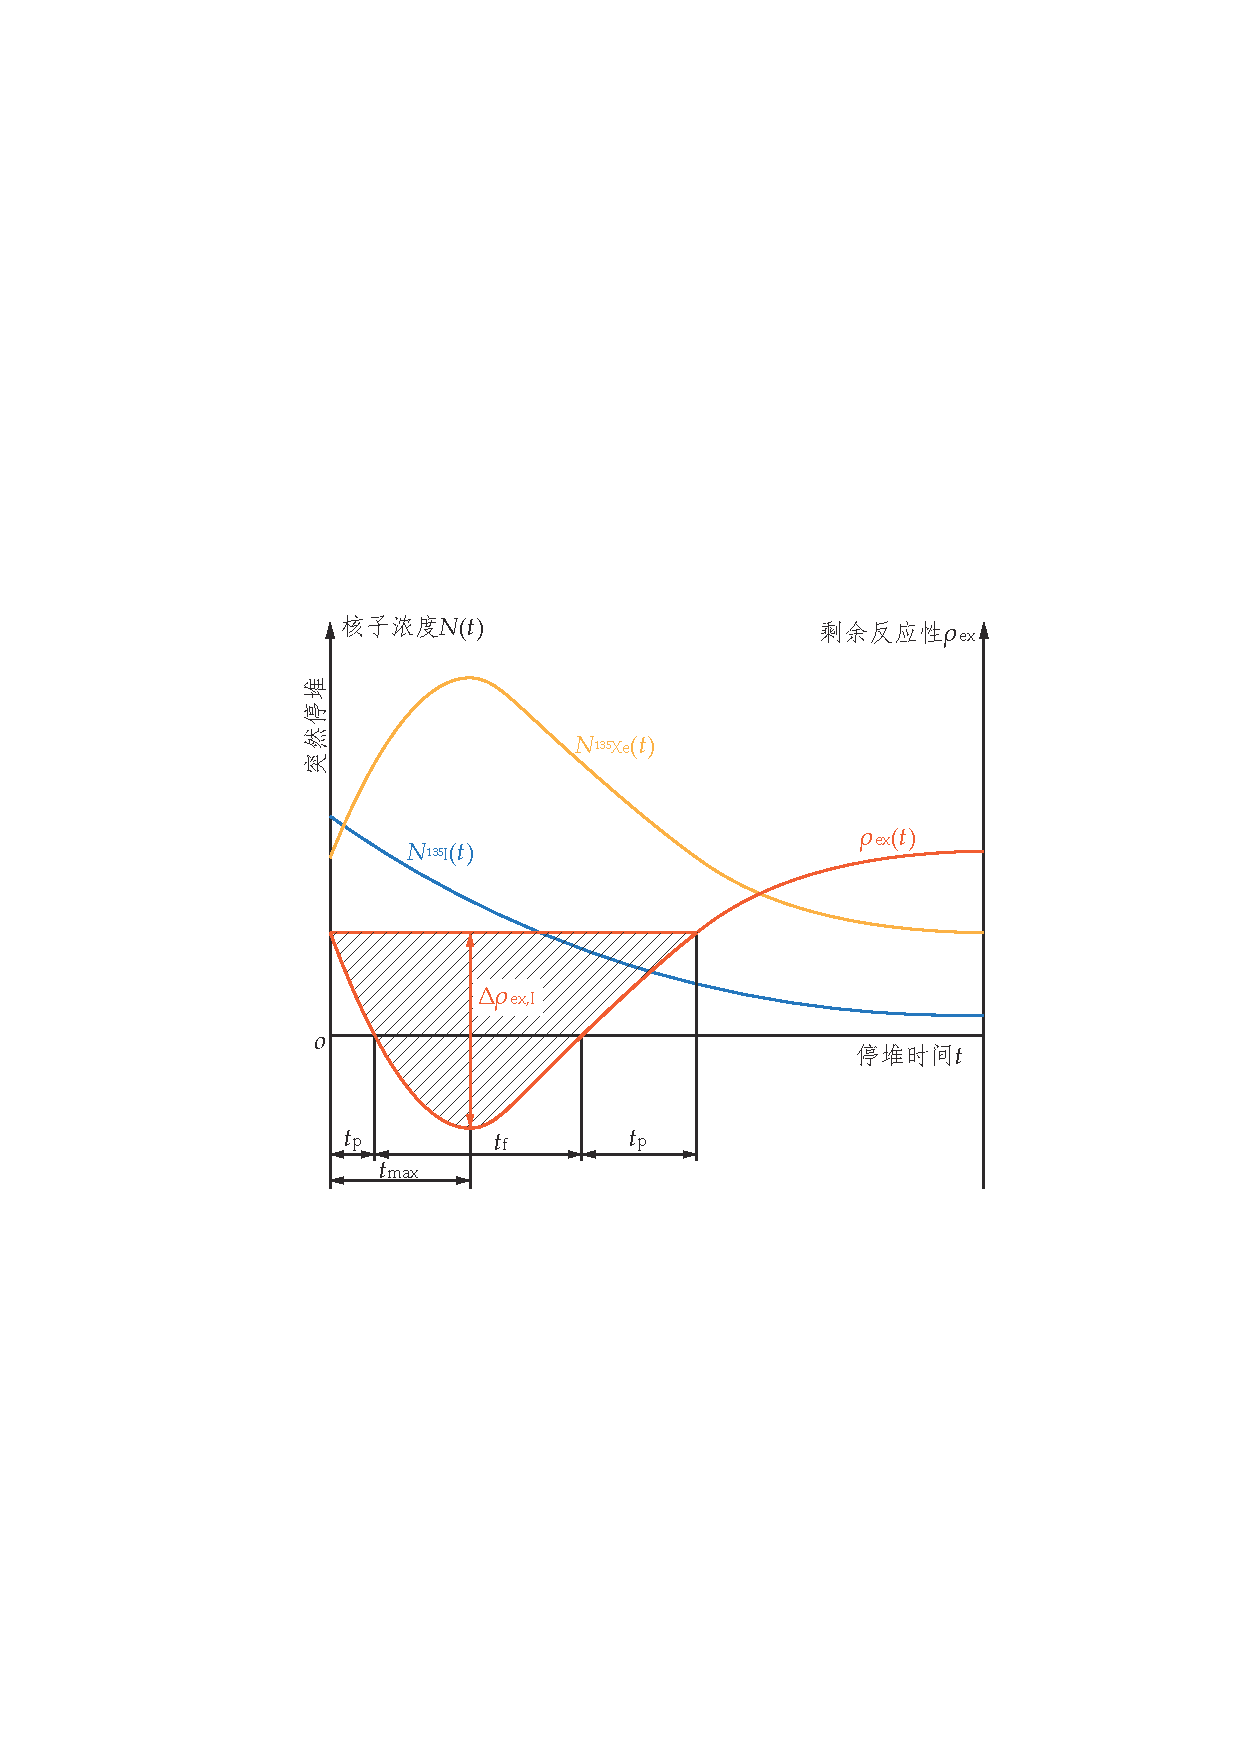
\includegraphics[scale=0.9]{figures/fig6.4.pdf}
        \end{figure}
    \end{solution}
\end{exercise}

\begin{exercise}
    一座压水堆,\,先以满功率运行200天,\,然后一次性将功率降至50\%FP,\,并稳定运行. 
    \begin{enumerate}[(1)]
        \item 试画出该过程中${}^{135}\symrm{I}$和${}^{135}\symrm{Xe}$的原子核密度随时间的变化曲线;
        \item 试画出该过程中${}^{149}\symrm{Pm}$和${}^{149}\symrm{Sm}$的原子核密度随时间的变化曲线.
    \end{enumerate}
    \begin{solution}
        \begin{enumerate}[(1)]
            \item 碘-氙
            \begin{figure}[H]
                \centering
                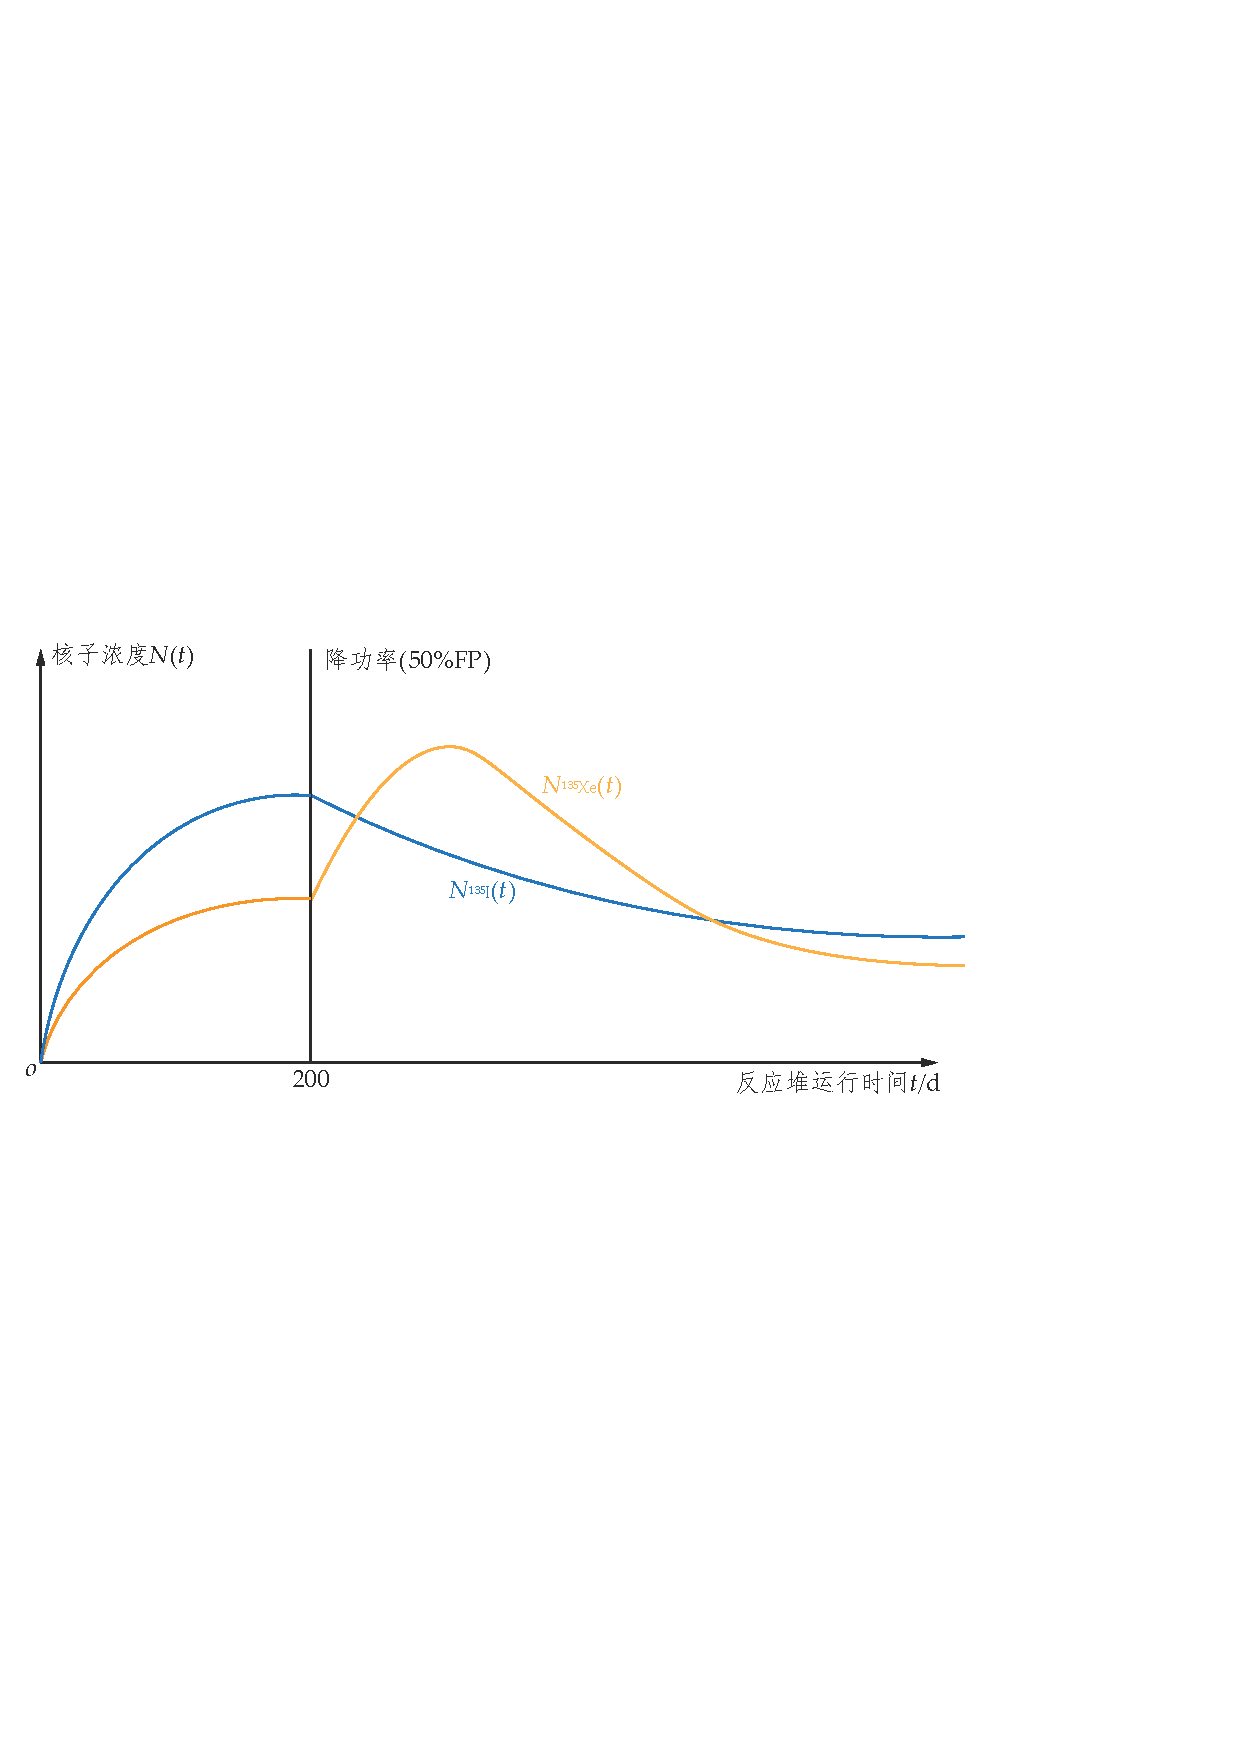
\includegraphics[scale=0.75]{figures/fig6.5.pdf}
            \end{figure}
            \item 钷-钐
            \begin{figure}[H]
                \centering
                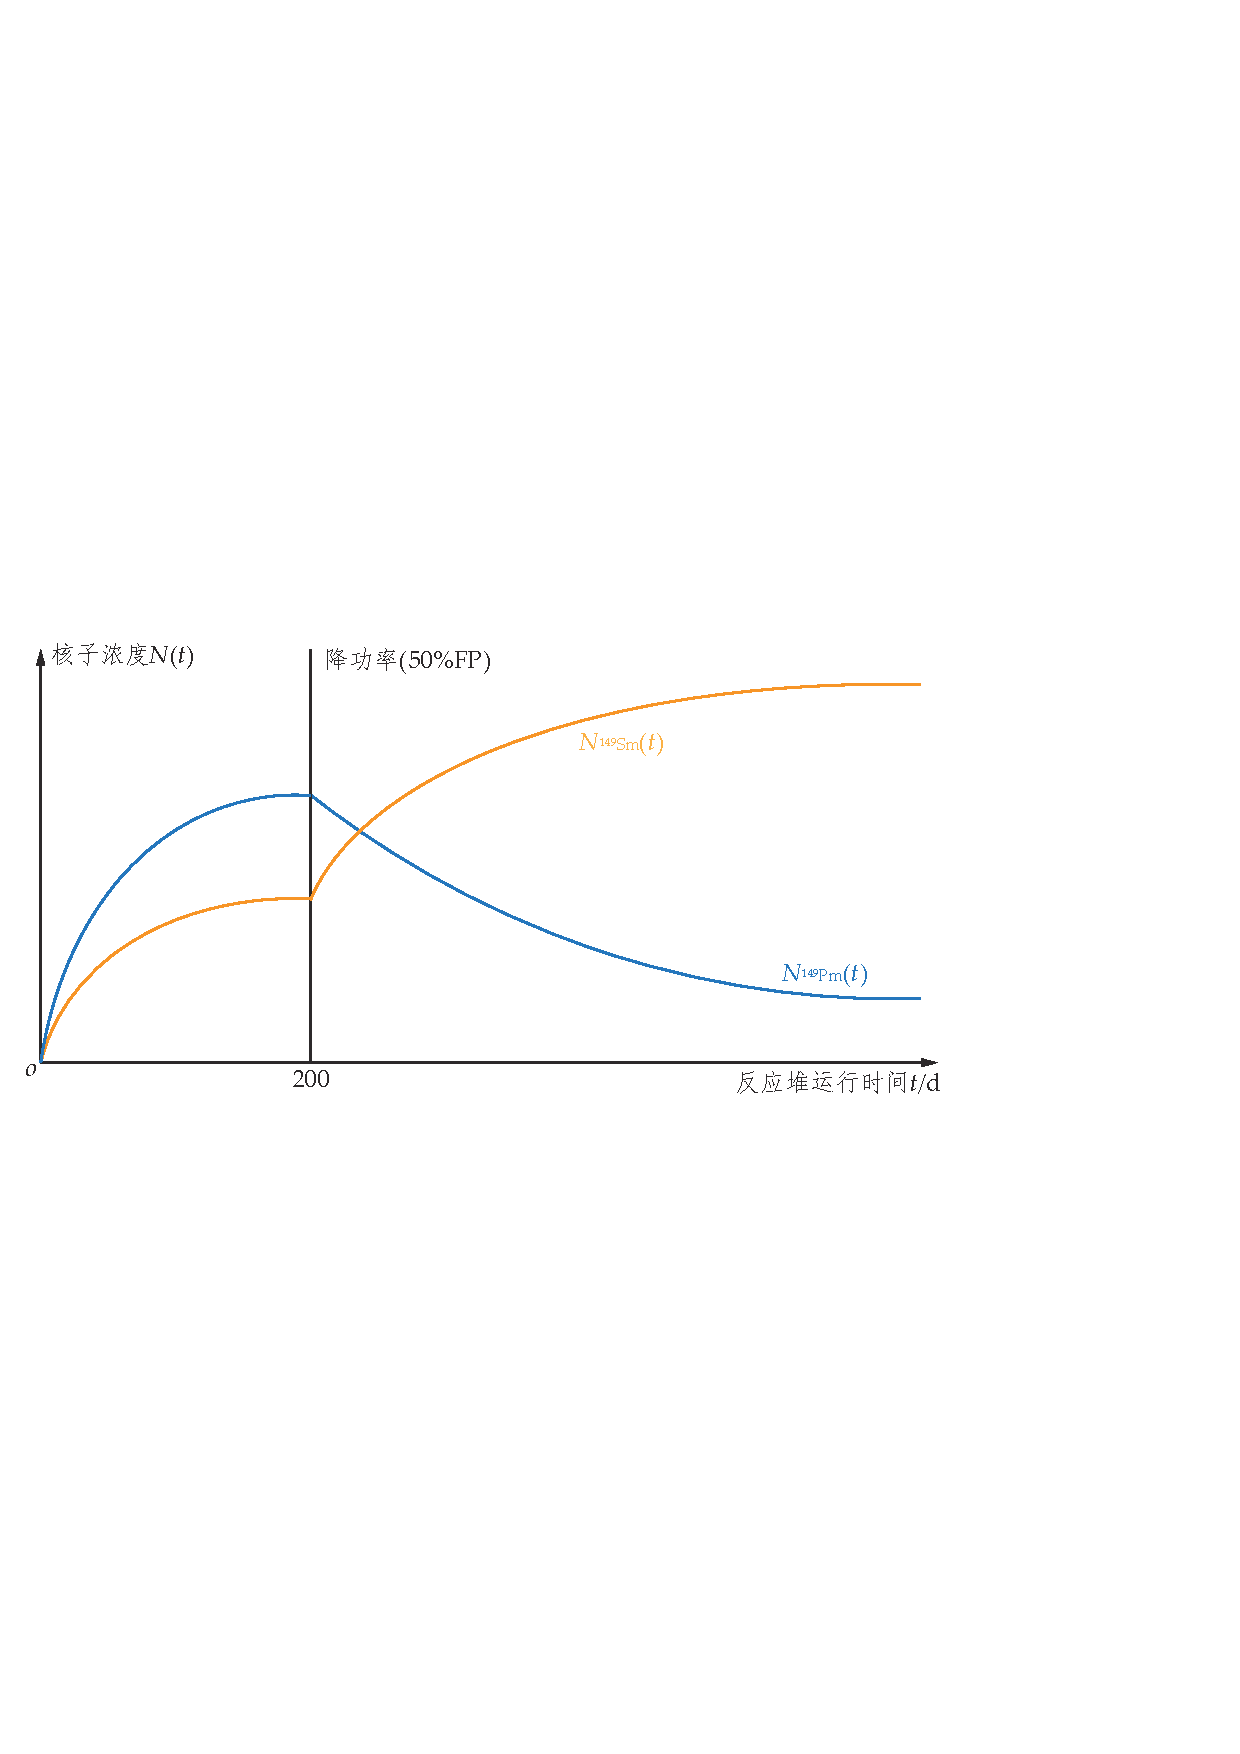
\includegraphics[scale=0.75]{figures/fig6.6.pdf}
            \end{figure}
        \end{enumerate}
    \end{solution}
\end{exercise}

\begin{exercise}
    试画出碘-氙衰变链,\,并根据平衡关系写出压水堆运行中碘和氙的原子核密度变化关系以及碘、氙的平衡浓度.\,
    \begin{solution}

        \begin{minipage}{0.2\columnwidth}
            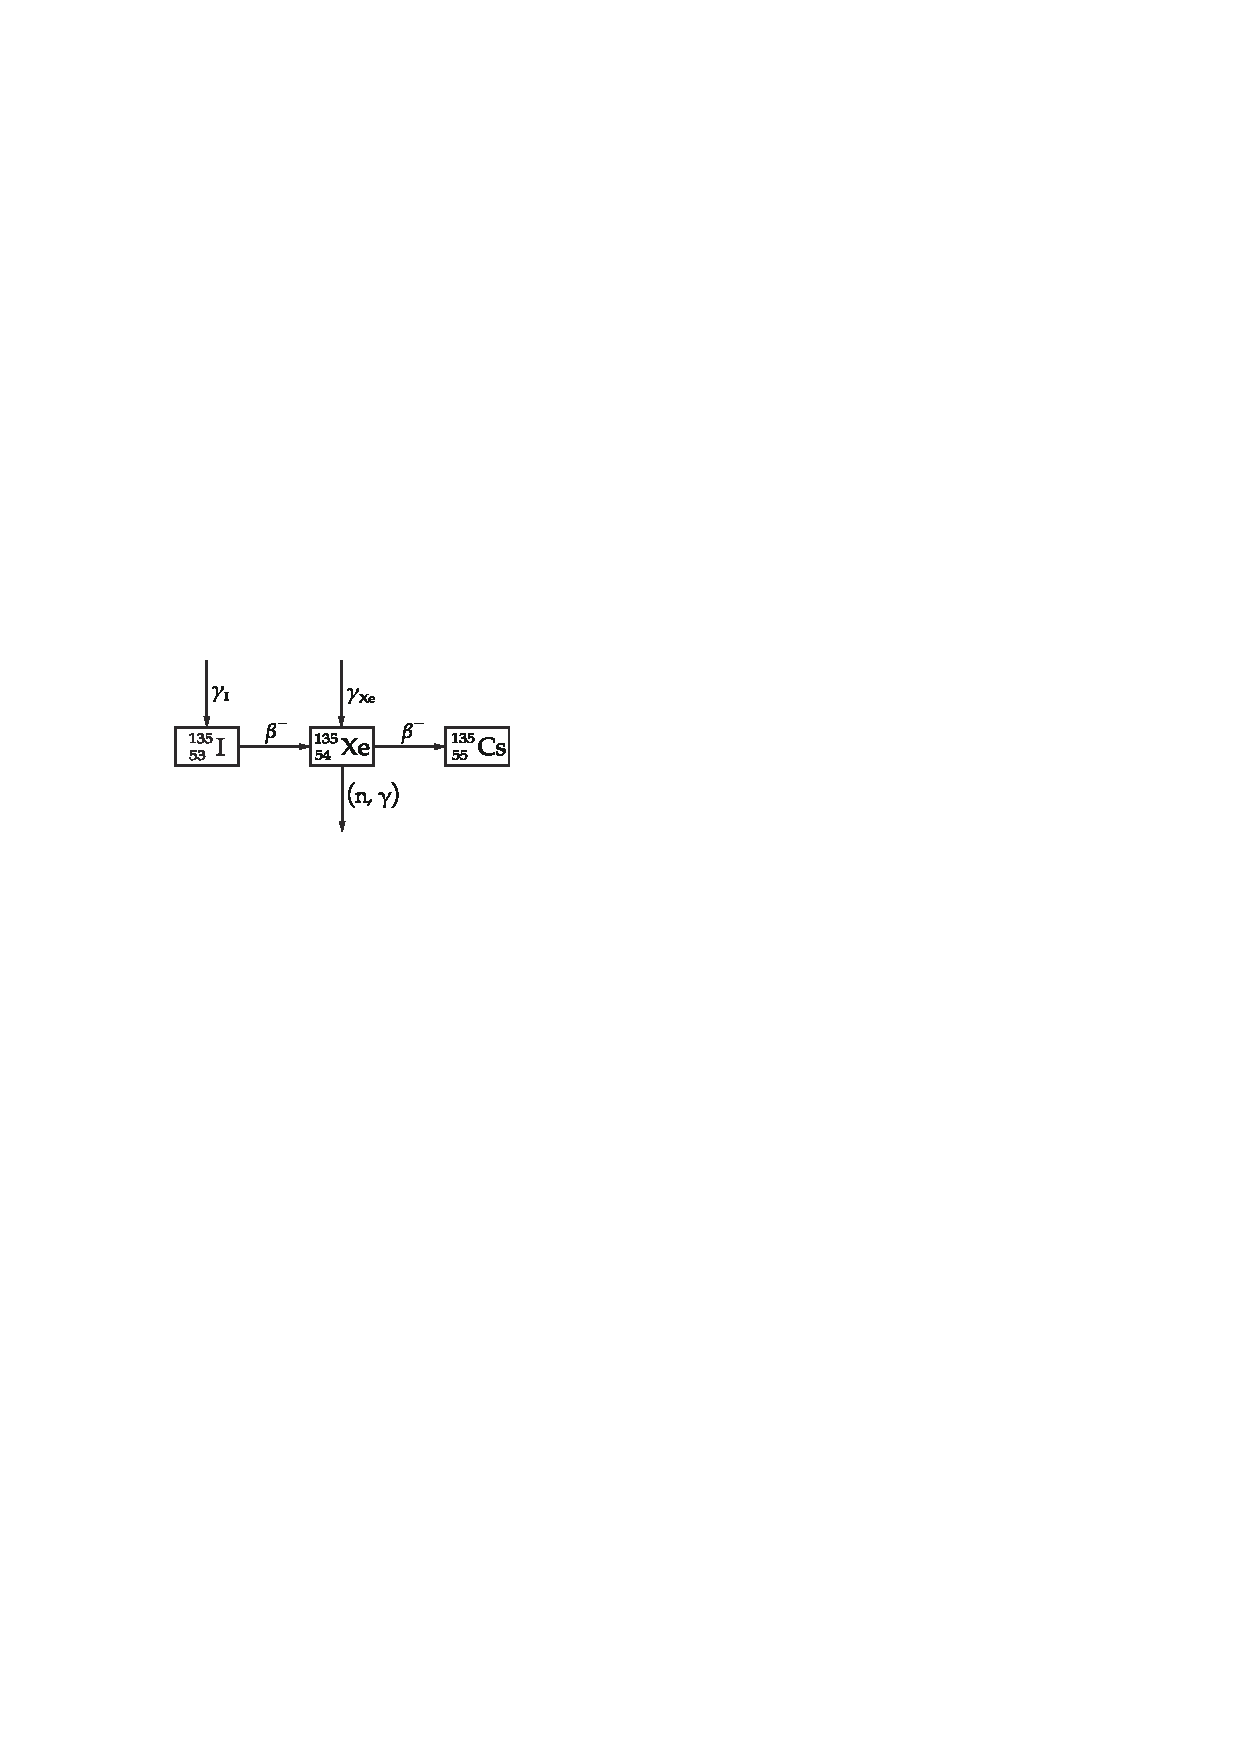
\includegraphics[scale=0.8]{figures/fig6.7.pdf}
        \end{minipage}
        \hfil
        \begin{minipage}{0.8\columnwidth}
            \begin{align*}
                & \dv{N_{\symrm{I}}(t)}{t} = \gamma_{\symrm{I}} \vSigma_{\symrm{f}} \phi - \lambda_{\symrm{I}} N_{\symrm{I}}(t) \\
                & \dv{N_{\symrm{Xe}}(t)}{t} = \gamma_{\symrm{Xe}} \vSigma_{\symrm{f}} \phi + \lambda_{\symrm{I}} N_{\symrm{I}}(t) - \left(\lambda_{\symrm{Xe}} + \sigma_{\gamma}^{\symrm{Xe}} \phi\right) N_{\symrm{Xe}}(t)
            \end{align*}
        \end{minipage}

        当$t \to \infty$,\,碘和氙达到平衡浓度时,\,$\dv{N_i(t)}{t} = 0$,\,于是
        \begin{align*}
            & N_{\symrm{I}}(\infty) = \frac{\gamma_{\symrm{I}} \vSigma_{\symrm{f}} \phi}{\lambda_{\symrm{I}}} \\
            & N_{\symrm{Xe}}(\infty) = \frac{(\gamma_{\symrm{I}} + \gamma_{\symrm{Xe}}) \vSigma_{\symrm{f}} \phi}{\lambda_{\symrm{Xe}} + \sigma_{\gamma}^{\symrm{Xe}}}
        \end{align*}
    \end{solution}
\end{exercise}

\begin{exercise}
    试画出钜-钐衰变链,\,并根据平衡关系写出压水堆运行中饱和钐的原子核密度变化关系以及钜和钐的平衡浓度.\,
    \begin{solution}

        \begin{minipage}{0.1\columnwidth}
            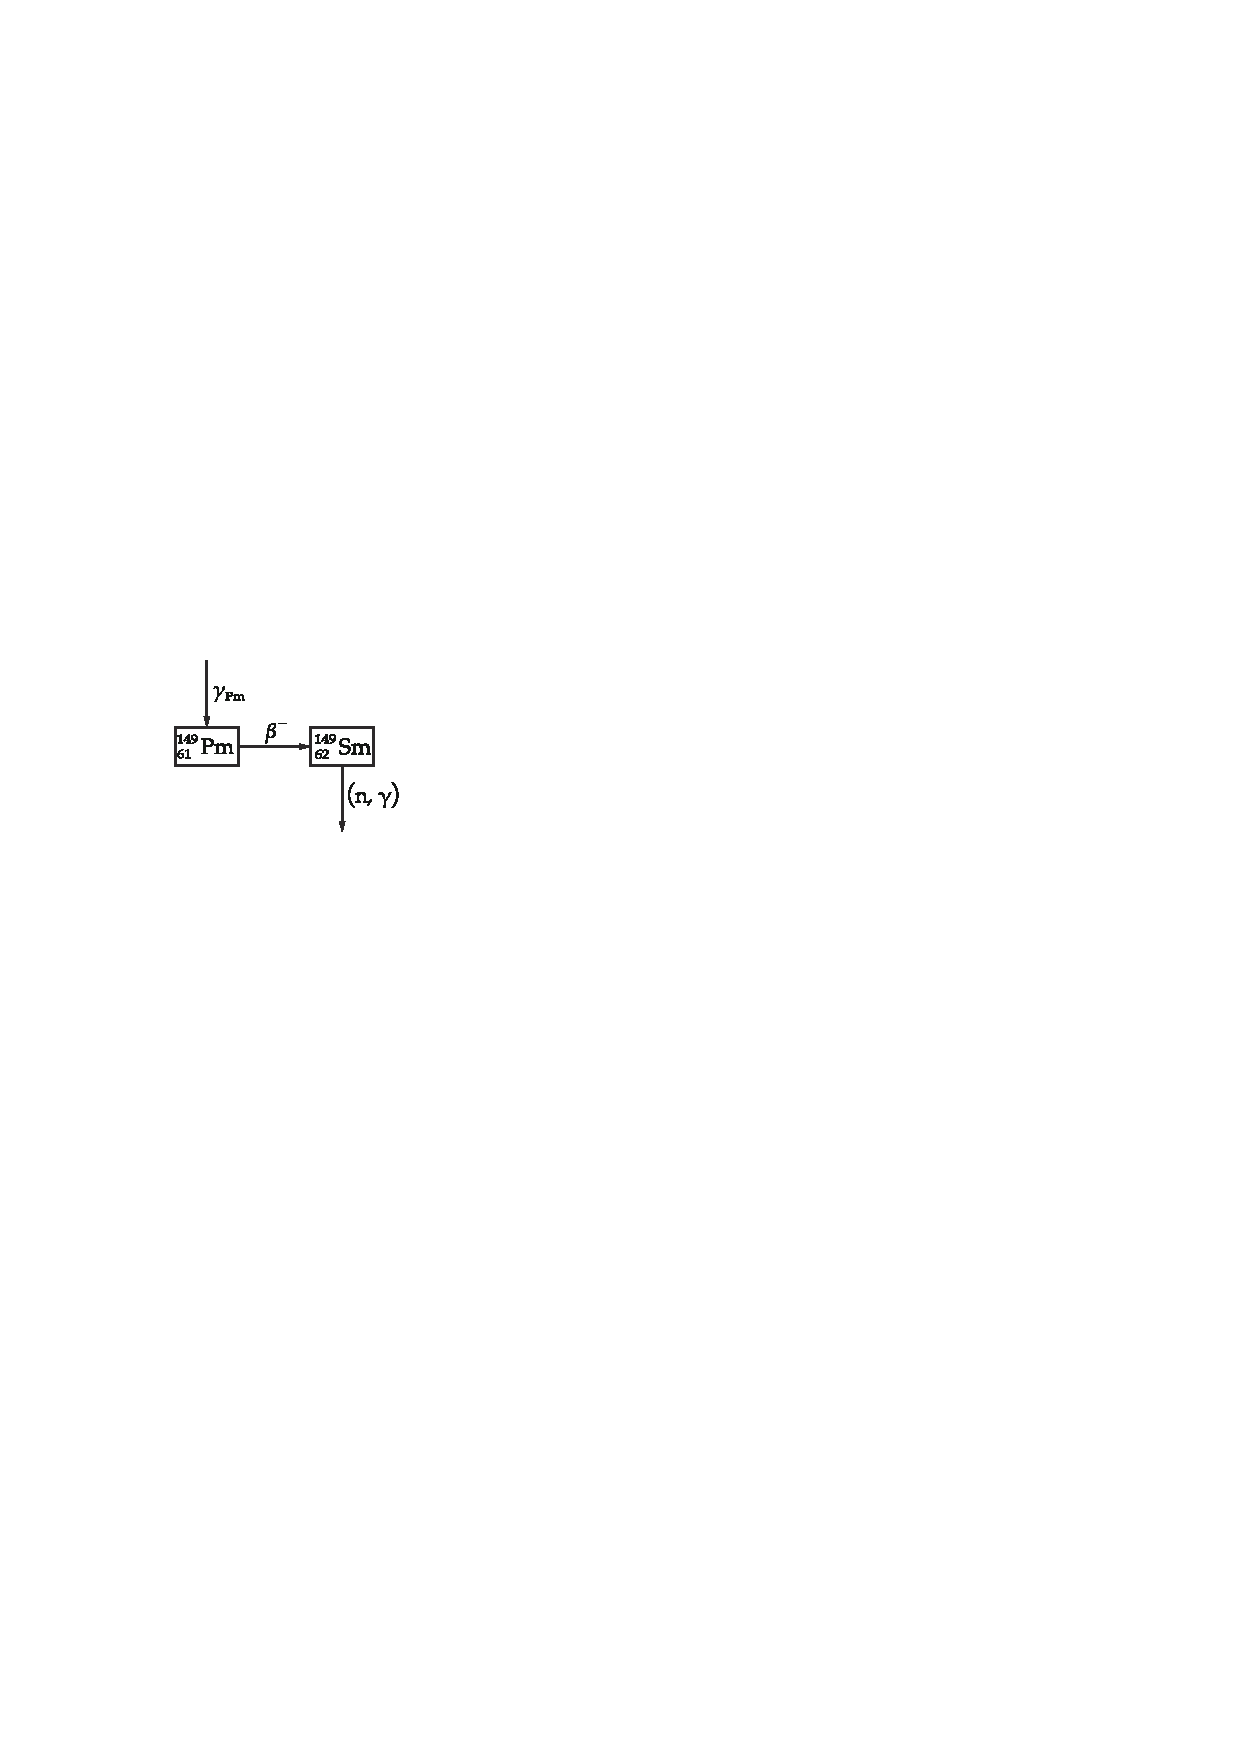
\includegraphics[scale=0.9]{figures/fig6.8.pdf}
        \end{minipage}
        \hfil
        \begin{minipage}{0.9\columnwidth}
            \begin{align*}
                & \dv{N_{\symrm{Pm}}(t)}{t} = \gamma_{\symrm{Pm}} \vSigma_{\symrm{f}} \phi - \lambda_{\symrm{Pm}} N_{\symrm{Pm}}(t) \\
                & \dv{N_{\symrm{Sm}}(t)}{t} = \lambda_{\symrm{Pm}} N_{\symrm{Pm}}(t) - \sigma_{\gamma}^{\symrm{Sm}} \phi N_{\symrm{Sm}}(t)
            \end{align*}
        \end{minipage}

        当$t \to \infty$,\,钷和钐达到平衡浓度时,\,$\dv{N_i(t)}{t} = 0$,\,于是
        \begin{align*}
            & N_{\symrm{Pm}}(\infty) = \frac{\gamma_{\symrm{Pm}} \vSigma_{\symrm{f}} \phi}{\lambda_{\symrm{Pm}}} \\
            & N_{\symrm{Sm}}(\infty) = \frac{\gamma_{\symrm{Pm}} \vSigma_{\symrm{f}}}{\sigma_{\gamma}^{\symrm{Sm}}}
        \end{align*}
    \end{solution}
\end{exercise}

\begin{exercise}
    一座热中子核反应堆,\,在低功率水平下运行到第42周时发生了紧急停堆,\,在12个小时后恢复临界,\,然后以一定的速率在6小时内将功率提升到60\%FP.\,为了在该水平下达到氙平衡状态,\,需要多长时间?\,\xparen
    \begin{xchoices}[showanswer=true]
        \item 20到30个小时
        \item* 40到50个小时
        \item 70到80个小时
        \item 不知道先前的功率运行史,\,不能确定需要多长时间
    \end{xchoices}
    \vspace{1em}
\end{exercise}

\begin{exercise}
    产生氙振荡的条件有哪些?\,
    \begin{solution}
        \begin{enumerate}[(1)]
            \item 核反应堆属于热中子反应堆;
            \item 核反应堆足够大.
        \end{enumerate}
    \end{solution}
\end{exercise}

\chapter{反应性系数与反应性控制}
\section*{习题}

\begin{exercise}
    名词解释:\,反应性系数,\,温度系数,\,空泡系数,\,功率系数,\,控制毒物价值,\,停堆裕量,\,控制棒价值,\,控制棒积分价值,\,控制棒微分价值,\,可燃毒物,\,硼微分价值,\,临界硼浓度.\,
    \begin{solution}
        \begin{enumerate}[(1)]
            \item 反应性系数:\,核反应堆的某个参数$x$发生单位变化所引起的反应性$\rho$的变化量;\,
            \item 温度系数:\,介质温度变化$1\,\symrm{K}$所引起的反应性变化量;\,
            \item 空泡系数:\,冷却剂中空泡份额变化1\% 所引起的反应性变化量;\,
            \item 功率系数:\,单位功率变化所引起的反应性变化量;\,
            \item 控制毒物价值:\,某一控制毒物全部投入堆芯所引起的反应性变化量,\,用$\rho_{\symrm{P}}$表示;\,
            \item 停堆裕量:\,堆芯冷态零功率条件下,\,考虑了堆芯功率降低引入的正反应性和价值最大的一束控制棒初始卡在高位的情况下,\,其余全部控制棒插入后反应堆将达到的次临界水平;\,
            \item 控制棒价值:\,控制棒全部插入堆芯所引起的反应性变化量;\,
            \item 控制棒积分价值:\,控制棒从堆外插至堆芯某一位置时所引起的反应性变化量;\,
            \item 控制棒微分价值:\,控制棒插入单位距离时所引起的反应性变化量;\,
            \item 可燃毒物:\,随核反应堆燃耗不断消耗能释放反应性的毒物;\,
            \item 硼微分价值:\,堆芯冷却剂中单位硼浓度变化所引起的反应性变化量;\,
            \item 临界硼浓度:\,在某一燃耗时刻,\,如果不考虑控制棒,\,完全用堆芯中的可燃毒物和可溶硼来控制,\,使得核反应堆处于临界所需要的硼浓度.\,
        \end{enumerate}
    \end{solution}
\end{exercise}

\begin{exercise}
    在压水堆冷却剂温度\underline{{\kaishu \,很低}}和压水堆硼浓度\underline{{\kaishu \,很高}}时,\,压水堆慢化剂温度系数负得最少.\,
\end{exercise}

\begin{exercise}
    某压水核反应堆系统在寿期初控制棒全提的时候$\keff = 1.023$,\,某组控制棒插入$10\,\symrm{cm}$时$\keff = 1.019$,\,则该组控制棒的微分价值为\xparen
    \begin{xchoices}[showanswer=true]
        \item 384 pcm/cm
        \item 400 pcm/cm
        \item 40.0 pcm/cm
        \item* 38.4 pcm/cm
    \end{xchoices}
    \vspace*{1em}
    \begin{solution}
        \begin{equation*}
            \left(\frac{\keff - 1}{\keff} - \frac{\keff' - 1}{\keff'}\right)/10\,\symrm{cm} = 38.4\,\symrm{pcm/cm}
        \end{equation*}
    \end{solution}
\end{exercise}

\begin{exercise}
    随着慢化剂温度的升高,\,控制棒微分价值变得更负,\,是因为\xparen
    \begin{xchoices}[showanswer=true]
        \item 慢化剂密度的减小造成更多的中子泄漏出堆芯
        \item 慢化剂温度系数降低,\,引起竞争减弱
        \item 燃料温度增加,\,中子在燃料中吸收减少
        \item* 慢化剂密度的减小使中子徙动长度增大
    \end{xchoices}
    \noindent {\color{third}{【注】}} {\kaishu 可参考:\,\faLink\,\hyperlink{https://www.fx361.cc/page/2019/0910/9929310.shtml}{https://www.fx361.cc/page/2019/0910/9929310.shtml}}
\end{exercise}

\begin{exercise}
    反应性控制的实质是什么?\,其主要任务、形式和途径有哪些?\,
    \begin{solution}
        \begin{enumerate}[(1)]
            \item 实质:\,维持堆内中子平衡关系;\,
            \item 主要任务:\,紧急控制,\,功率调节,\,燃耗补偿;\,
            \item 形式:\,改变堆内中子的吸收,\,产生和泄漏;\,
            \item 途径:\,(改变中子吸收)控制棒,\,可燃毒物,\,可溶硼.\,
        \end{enumerate}
    \end{solution}
\end{exercise}

\begin{exercise}
    一核反应堆在寿期末从100\%\,FP功率运行状态下停堆,\,经过3天冷却至$333\,{}^{\circ}\symrm{C}$,\,在冷却期间,\,硼浓度增加了100\,ppm.\,在停堆与冷却期间所添加的反应性绝对值如下所示.\,请在括号中填入适当的符号($+$或$-$),\,并计算当前的次临界深度.\,

    控制棒 =($-$)$6.918\%\,\Delta k/k$

    氙 =($+$)$2.675\%\,\Delta k/k$

    功率亏损 =($+$)$1.575\%\,\Delta k/k$

    硼 = ($-$) $1.040\%\,\Delta k/k$

    温度 =($+$)$0.500\%\,\Delta k/k$
    \begin{solution}
        当前次临界深度
        \begin{equation*}
            - 6.918\% + 2.675\% + 1.575\% - 1.040\% + 0.500\% = -3.208\%\,\Delta k/k
        \end{equation*}
    \end{solution}
\end{exercise}

\begin{exercise}
    一核反应堆在80\%\,FP功率运行时,\,操作员向核反应堆冷却剂系统(RCS)中添加10 加仑(gal)的硼酸,\,经过若干分钟,\,操作员按需要调节控制棒的位置,\,以维持核反应堆冷却剂平均温度不变.\,当电厂处于稳定状态时,\,停堆裕量将\underline{{\kaishu \,增加}},\,而轴向功率峰将移向堆芯的\underline{{\kaishu \,上方}}.\,
\end{exercise}

\begin{exercise}
    已知参数为:\,核反应堆功率$=100\%\,\symrm{FP}$,\,总功率系数$ = -0.020\%\,\Delta k/k/\,\%\,\symrm{FP}$,\,初始硼浓度$=500\,\symrm{ppm}$,\,硼价值$=-0.010\%\,\Delta k/k/\,\symrm{ppm}$,\,控制棒价值$ = -0.010\%\,\Delta k/k/\,\symrm{cm}$(插入),\,试问通过硼化/稀释、控制插入$50\,\symrm{cm}$、使电厂功率降至$30\%\,\symrm{FP}$所要求的最终硼浓度是多少(假设堆芯的其他状态参数不变)?\,
    \begin{solution}
        功率降至30\%\,FP引入反应性
        \begin{equation*}
            \Delta\rho = -0.020\%\,\Delta k/k/\,\%\,\symrm{FP} \times \left(30\%\,\symrm{FP} - 100\%\,\symrm{FP}\right) = 1.4\%\,\Delta k/k
        \end{equation*}
        控制棒插入$50\,\symrm{cm}$引入反应性
        \begin{equation*}
            \Delta\rho_{\symrm{r}} = -0.010\%\,\Delta k/k/\,\symrm{cm} \times 50\,\symrm{cm} = -0.5\%\,\Delta k/k
        \end{equation*}
        设最终硼浓度为$c$,\,则硼浓度变化引入反应性
        \begin{equation*}
            \Delta\rho_{\symrm{B}} = -0.010\%\,\Delta k/k/\,\symrm{ppm} \times (c-500)\,\symrm{ppm} = -0.010(c-500)\%\,\Delta k/k
        \end{equation*}
        而$\Delta\rho + \Delta\rho_{\symrm{r}} + \Delta\rho_{\symrm{B}} = 0$,\,解得
        \begin{equation*}
            c = \frac{\Delta\rho + \Delta\rho_{\symrm{r}}}{-0.010} + 500\,\symrm{ppm} = \frac{1.4 - 0.5}{-0.01} + 500\,\symrm{ppm} = 590\,\symrm{ppm}
        \end{equation*}
        即经过硼稀释,\,最终硼浓度为$590\,\symrm{ppm}$.\,
    \end{solution}
\end{exercise}

\begin{exercise}
    用提升控制棒外推临界棒位时,\,若该棒组提升12步使得源量程计数从$n_1$增加到$n_2$且$n_2 = 1.5 n_1$.\,假定控制棒微分价值为常数,\,试估算还需提升该棒组多少步才能达到临界?\,
    \begin{solution}
        设还需提升该棒组$x$步才能达到临界,\,由倒计数率法,\,有
        \begin{equation*}
            \frac{1/n_1 - 1/n_2}{12} = \frac{1/n_2 - 0}{x}
        \end{equation*}
        且$n_2 = 1.5 n_1$,\,解得
        \begin{equation*}
            x = 24
        \end{equation*}
        故还需提升该棒组24步才能达到临界.\,
    \end{solution}
\end{exercise}

\begin{exercise}
    为什么压水堆选择设计成欠慢化?\,
    \begin{solution}
        压水堆设计成欠慢化,\,慢化剂温度为负,\,当反应堆功率升高时,\,温度升高,\,水-铀比减小,\,则此时引入负反应性,\,使功率自稳自调,\,即这样的设计是一种固有安全特性.\,
    \end{solution}
\end{exercise}

\chapter{核反应堆动力学}
\section*{习题}

\begin{exercise}
    名词解释:\,热中子寿期,\,核反应堆周期,\,瞬发临界,\,次临界度.\,
    \begin{solution}
        \begin{enumerate}
            \item 热中子寿期:\,热中子被吸收前所花费的时间;\,
            \item 核反应堆周期:\,中子密度增加到原来的e倍所需要的时间,\,用$T$表示;\,
            \item 瞬发临界:\,$\rho = \beta$,\,仅靠瞬发中子,\,核反应堆就会达到临界;\,
            \item 次临界度:\,有效增殖系数与1的距离,\,即$1 - \keff$.\,
        \end{enumerate}
    \end{solution}
\end{exercise}

\begin{exercise}
    某核反应堆中子密度随时间的变化可以表示为$n(t) = A_0 \symrm{e}^{\omega_1 t} + A_1 \symrm{e}^{\omega_2 t}$,\,则其核反应堆周期为\xparen
    \begin{xchoices}[showanswer=true]
        \item $T(t) = A_0 \symrm{e}^{\omega_1 t} + A_1 \symrm{e}^{\omega_2 t}$
        \item $T(t) = A_0 \omega_1 \symrm{e}^{\omega_1 t} + A_1 \omega_2 \symrm{e}^{\omega_2 t}$
        \item $\displaystyle T(t) = \frac{A_0 \omega_1 \symrm{e}^{\omega_1 t} + A_1 \omega_2 \symrm{e}^{\omega_2 t}}{A_0 \symrm{e}^{\omega_1 t} + A_1 \symrm{e}^{\omega_2 t}}$
        \item* $\displaystyle T(t) = \frac{A_0 \symrm{e}^{\omega_1 t} + A_1 \symrm{e}^{\omega_2 t}}{A_0 \omega_1 \symrm{e}^{\omega_1 t} + A_1 \omega_2 \symrm{e}^{\omega_2 t}}$
    \end{xchoices}
    
    \vspace*{2em}
    
    \begin{solution}
        \begin{equation*}
            T(t) = \frac{n(t)}{\symrm{d}n(t)/\symrm{d}t} = \frac{A_0 \symrm{e}^{\omega_1 t} + A_1 \symrm{e}^{\omega_2 t}}{A_0 \omega_1 \symrm{e}^{\omega_1 t} + A_1 \omega_2 \symrm{e}^{\omega_2 t}}
        \end{equation*}
    \end{solution}
\end{exercise}

\begin{exercise}
    试根据中子平衡关系写出点堆动力学方程并简述其适用范围.\,
    \begin{solution}
        中子密度变化率 = 产生率(瞬发+缓发) - 消失率(泄漏+吸收)
        \begin{equation*}
            \tikzmarknode{n}{\highlight{red}{$\dv{n(t)}{t}$}} =
            \color{BlueViolet}
            \overbrace{
                \left(\tikzmarknode{sf}{\highlight{Plum}{\color{black} $k \frac{n}{l} (1-\beta)$}} {\color{black} +} \tikzmarknode{hf}{\highlight{NavyBlue}{\color{black}  $\sum\limits_{i=1}^{6} \lambda_i C_i(t)$}}\right)
            }^{\text{\fangsong \footnotesize \textcolor{BlueViolet!85}{中子的产生率(瞬发+缓发)}}}
                \color{black} - 
                \tikzmarknode{xs}{\highlight{Bittersweet}{\color{black} $\frac{n}{l}$}}
        \end{equation*}
        \vspace*{0.5\baselineskip}
        \begin{tikzpicture}[overlay,remember picture,>=stealth,nodes={align=left,inner ysep=1pt},<-]
            % 中子密度变化率
            \path (n.north) ++ (0,0.5em) node[anchor=south east,color=Maroon!85] (ntext){\fangsong{\footnotesize 中子密度变化率}};
            \draw [color=Maroon](n.north) |- ([xshift=-0.3ex,color=Maroon]ntext.south west);
            % 瞬发中子的产生
            \path (sf.north) ++ (-2.4,-2.2em) node[anchor=north west,color=Plum!85] (sftext){{\fangsong{\footnotesize 瞬发中子的产生}}};
            \draw [color=Plum](sf.south) |- ([xshift=-0.3ex,color=Plum]sftext.south west);
            % 缓发中子的产生
            \path (hf.north) ++ (-2.4,-4.2em) node[anchor=north west,color=NavyBlue!85] (hftext){{\fangsong{\footnotesize 缓发中子的产生}}};
            \draw [color=NavyBlue](hf.south) |- ([xshift=-0.3ex,color=NavyBlue]hftext.south west);
            % 中子的消失(泄漏+消失)
            \path (xs.north) ++ (0.1,-3.2em) node[anchor=north west,color=Bittersweet!85] (xstext){\fangsong{\footnotesize 中子的消失(泄漏+消失)}};
            \draw [color=Bittersweet](xs.south) |- ([xshift=-0.3ex,color=Bittersweet]xstext.south east);
        \end{tikzpicture}

        缓发中子先驱核浓度变化率 = 产生率(裂变) + 消失率(衰变)
        \vspace*{1em}
        \begin{equation*}
            \tikzmarknode{C}{\highlight{red}{$\dv{C_i(t)}{t}$}} =
            \tikzmarknode{lb}{\highlight{Plum}{\color{black} $\beta_i k \frac{n}{l}$}} {\color{black} -} \tikzmarknode{sb}{\highlight{NavyBlue}{\color{black}  $\lambda_i C_i(t)$}}\quad {\color{black} i = 1,\,2,\,\cdots,\,6}
        \end{equation*}
        \vspace*{0.5\baselineskip}
        \begin{tikzpicture}[overlay,remember picture,>=stealth,nodes={align=left,inner ysep=1pt},<-]
            % 缓发中子先驱核浓度变化率
            \path (C.north) ++ (0,0.5em) node[anchor=south east,color=Maroon!85] (Ctext){\fangsong{\footnotesize 缓发中子先驱核浓度变化率}};
            \draw [color=Maroon](C.north) |- ([xshift=-0.3ex,color=Maroon]Ctext.south west);
            % 缓发中子先驱核的产生(裂变)
            \path (lb.north) ++ (-4.2,-2.2em) node[anchor=north west,color=Plum!85] (lbtext){{\fangsong{\footnotesize 缓发中子先驱核的产生(裂变)}}};
            \draw [color=Plum](lb.south) |- ([xshift=-0.3ex,color=Plum]lbtext.south west);
            % 缓发中子先驱核的消失(衰变)
            \path (sb.north) ++ (0.1,-2.2em) node[anchor=north west,color=NavyBlue!85] (sbtext){{\fangsong{\footnotesize 缓发中子先驱核的消失(衰变)}}};
            \draw [color=NavyBlue](sb.south) |- ([xshift=-0.3ex,color=NavyBlue]sbtext.south east);
        \end{tikzpicture}

        \newpage
        令$\vLambda = l/k$为中子代时间,\,则
        \begin{align*}
            &\dv{n}{t} = \frac{\rho - \beta}{\vLambda}n + \sum_{i=1}^{6} \lambda_i C_i(t) \\
            &\dv{C_i(t)}{t} = \frac{\beta_i}{\vLambda}n - \lambda_i C(i) \quad i = 1,\,2,\,\cdots,\,6
        \end{align*}

        适用范围:\,只关注中子密度随时间的变化,\,忽略其随空间的变化,\,即点堆模型.\,

    \end{solution}
\end{exercise}

\begin{exercise}
    试从中子平衡方程导出瞬发临界的条件.\,
    \begin{solution}
        瞬发临界,\,即不考虑缓发中子且达到临界,\,于是
        \begin{equation*}
            \dv{n}{t} = \frac{\rho - \beta}{\vLambda}n = 0 \Rightarrow \rho = \beta
        \end{equation*}
    \end{solution}
\end{exercise}

\begin{exercise}
    在核反应堆启动过程中,\,在操作员未进行任何操作的情况下,\,核反应堆功率在两分钟之内从$3\times 10^{-6}\%\,\symrm{FP}$增加到$5\times 10^{-6}\%\,\symrm{FP}$,\,则功率增长过程中的平均核反应堆周期是多少秒?
    \begin{solution}
        核反应堆在启堆阶段低功率水平下不考虑缓发中子,\,则中子密度满足
        \begin{equation*}
            n(t) = n_0 \symrm{e}^{t/T}
        \end{equation*}
        核反应堆功率$P$与中子密度$n$成正比,\,即有
        \begin{align*}
                        &\frac{n_0 \symrm{e}^{(t+120)/T}}{n_0 \symrm{e}^{t/T}} = \frac{5\times 10^{-6}}{3\times 10^{-6}} \\
            \Rightarrow & T = \frac{120}{\loge (5/3)}\,\symrm{s} = 234.91\,\symrm{s}
        \end{align*}
    \end{solution}
\end{exercise}

\begin{exercise}
    向一个处于停堆状态的核反应堆中添加某个正反应性后,\,尽管此时的$\keff < 1$,\,但观察到中子计数率在增长,\,这种现象的起因是\xparen
    \begin{xchoices}[showanswer=true]
        \item 缓发中子
        \item 等温温度系数
        \item 中子慢化
        \item* 次临界增殖
    \end{xchoices}
\end{exercise}

\begin{exercise}
    缓发中子对核反应堆的稳定性贡献比瞬发中子大,\,是因为它们使中子平均代时间\underline{延长},\,并且它们在诞生时具有\underline{更低}的动能.\,
\end{exercise}

\begin{exercise}
    在核反应堆启动期间,\,当硼浓度为$C_{\symrm{B}} = 1500\,\symrm{ppm}$时,\,平均计数率为$n_1$,\,且已知此时堆芯的$k_{\symrm{eff,1}} = 0.97$;\,当硼浓度稀释到$C_{\symrm{B}} = 1260\,\symrm{ppm}$时,\,平均计数率为$n_2$;\,若$n_2 = 5n_1$,\,试估算在此期间因硼稀释引进了多少pcm的反应性?
    \begin{solution}
        核反应堆启动趋近临界时满足次临界公式,\,即
        \begin{equation*}
            N = \frac{S_0}{1-\keff}
        \end{equation*}
        由题意,\,得
        \begin{align*}
            &n_1 = \frac{S_0}{1-k_{\symrm{eff,1}}} \\
            &n_2 = \frac{S_0}{1-k_{\symrm{eff,2}}} = 5 n_1
        \end{align*}
        解得$k_{\symrm{eff,2}} = 0.994$.\,由$\rho = (\keff - 1)/\keff$,\,得
        \begin{equation*}
            \rho_1 = -3092.8\,\symrm{pcm},\;\rho_2 = -603.62\,\symrm{pcm}
        \end{equation*}
        引入反应性$\Delta \rho = \rho_2 - \rho_1 = 2489.2\,\symrm{pcm}$.\,
    \end{solution}
\end{exercise}

\chapter{堆芯核燃料管理}
\section*{习题}

\begin{exercise}
    名词解释:\,循环长度,\,换料周期,\,多循环燃料管理,\,单循环燃料管理,\,初始循环,\,平衡循环,\,过渡循环,\,线性反应性模型,\,增殖比,\,次锕系核素,\,长寿命裂变产物,\,核废料嬗变,\,闭式燃料循环.\,
    \begin{solution}
        \begin{enumerate}[(1)]
            \item 循环长度:\,一次装料后,\,核反应堆能满功率运行的时间;\,
            \item 换料周期:\,核反应堆两次停堆换料之间的时间间隔;\,
            \item 多循环燃料管理:\,燃料组件在堆芯内的空间影响仅以“批”的特性简单考虑,\,而在时间上可以考虑多个循环;\,
            \item 单循环燃料管理:\,详细考虑燃料组件和控制毒物在堆芯内的空间布置,\,可以不考虑各循环之间的相互影响;\,
            \item 初始循环:\,核反应堆首次启动运行的第一个循环,\,堆芯全部由新燃料组成;\,
            \item 平衡循环:\,每个循环的性能参数都保持相同,\,运行循环进入到一个平衡状态;\,
            \item 过渡循环:\,从第2循环开始一直延续到平衡循环为止的各个循环;\,
            \item 线性反应性模型:\,对于典型轻水堆燃料组件,\,其反应性$\rho$可近似为燃料燃耗深度的线性递减函数,\,即
            \begin{equation*}
                \rho_i(B) = \rho_{0,i} - \alpha_i B_i
            \end{equation*}
            \item 增殖比:\,转换比(CR)>1时的转换比称为增殖比,\,用BR表示;\,
            \item 次锕系核素:\,除去U和Pu以外的其他锕系元素,\,简称MA;\,
            \item 长寿命裂变产物:\,半衰期特别长,\,已远远超出人类管理范围的裂变产物;\,
            \item 核废料嬗变:\,通过中子俘获反应,\,把长寿命高放同位素变成短寿命或稳定同位素;\,
            \item 闭式燃料循环:\,核燃料从地质勘探、采矿、铀浓缩、燃料组件制造到核反应堆内燃烧、后处理、地质贮存等过程,\,形成一个封闭的核燃料循环.\,
        \end{enumerate}
    \end{solution}
\end{exercise}

\begin{exercise}
    设一座核反应堆由$n = 3$批料组成,\,假设反应性随燃耗线性减少,\,且其斜率与初始富集度无关,\,各批料以相同功率密度运行,\,初始循环的循环燃耗与以后各循环的相等,\,从第2循环开始新料的富集度就取成平衡循环的换料富集度,\,请确定各批料的初始反应性.\,
    \begin{solution}
        设循环燃耗深度为$B_n^c$,\,每批料反应性变化斜率为$\alpha$,\,根据满功率运行循环寿期末堆芯反应性为0,\,根据线性反应性模型$\rho_i(B) = \rho_{0,i} - \alpha_i B_i$,\,得
        \begin{equation*}
            \rho_0 - \frac{1}{n}\sum_{i=1}^{n} i \alpha B_n^c = 0
        \end{equation*}
        于是有循环燃耗为
        \begin{equation*}
            B_n^c = \frac{2\rho_0}{(n+1)\alpha}
        \end{equation*}
        进一步,\,卸料燃耗为
        \begin{equation*}
            B_n^d = n B_n^c = \frac{2n}{n+1}B_1^d = \frac{2n}{n+1}B_1^c = \frac{2n\rho_0}{(n+1)\alpha}
        \end{equation*}
        则初始反应性
        \begin{equation*}
            \rho_0 = \frac{n+1}{2n} \alpha B_n^d = \frac{n+1}{2} \alpha B_n^c = 2\alpha B_3^c
        \end{equation*}
    \end{solution}
\end{exercise}

\begin{exercise}
    试从我国国情出发论述我国发展快堆的必要性.\,
    \begin{solution}
        我国铀矿储量少,\,核废料处理技术发展尚不成熟.\,快堆在释放能量的时候同时能够核燃料增殖,\,还能将乏燃料中的长寿命废料变成短寿命废料.\,这是实现我国核能可持续发展的关键.\,
    \end{solution}
\end{exercise}

\chapter{核反应堆物理设计和启动物理试验}
\section*{习题}

\begin{exercise}
    在满足设计准则的基础上,\,堆芯物理设计的内容主要有哪些?\,
    \begin{solution}
        \begin{enumerate}[(1)]
            \item 堆芯栅格和装载方案设计;\,
            \item 反应性控制方案设计;\,
            \item 堆芯燃料管理方案设计.\,
        \end{enumerate}
    \end{solution}
\end{exercise}

\begin{exercise}
    什么是核反应堆功率能力?\,
    \begin{solution}
        核反应堆功率能力是在设计阶段或生产阶段,\,核反应堆设计能够提供的最大热输出功率,\,也就是反应堆的理论上限.\,它主要受到反应堆的几何形状、材料属性、燃料特性、系统配置等因素的影响.\,这个数值主要用于计算反应堆的设计和性能评估,\,对于现有的反应堆,\,没有改变反应堆结构和运行条件的情况下,\,其核反应堆功率能力是固定的.\,
    \end{solution}
\end{exercise}

\begin{exercise}
    建立保护梯形、运行梯形的依据是什么?\,思路如何?\,
    \begin{solution}
        \begin{enumerate}[(1)]
            \item 运行梯形图:通过计算足够多的两类工况下的堆芯轴向功率分布,\,可以给出堆芯不同状态下功率峰因子与轴向功率偏移$AO$的对应关系,\,再由这一关系导出\uppercase\expandafter{\romannumeral1}类工况的轴向功率偏差对堆芯功率变化的梯形限制区.\,
            \item 超功率保护梯形图:在\uppercase\expandafter{\romannumeral2}类工况下保证燃料棒的完整性而限制的最大线功率密度,\,同样为轴向功率偏差对堆芯功率变化的梯形限制区.\,
        \end{enumerate}
        运行梯形图和超功率保护梯形图给出了核反应堆在不同功率分布条件下的功率输出范围.\,
    \end{solution}
\end{exercise}

\begin{exercise}
    正常启动到临界过程中主要注意哪几点?\,
    \begin{solution}
        \begin{enumerate}[(1)]
            \item 这一过程需要确定临界条件,\,包括控制棒的临界棒位以及临界硼浓度.\,
            \item 在启动过程中,\,需要在堆芯内装载中子源将核反应堆在启动和趋近临界过程中很低的中子注量率水平放大到中子计数器可监控的水平,\,使得整个核反应堆趋近临界的过程处于监督之下,\,避免核反应堆启动“盲区”.\,
        \end{enumerate}
    \end{solution}
\end{exercise}


\clearpage
\phantom{s}
\thispagestyle{empty}

\includepdf{cover2.pdf}

\end{document}